% Define some commonly used terms.
% We did include xcolor, didn't we?
\newcommand{\vyse}{\textcolor{blue}{$V_{yse}$ }}
\newcommand{\vmc}{\textcolor{red}{$V_{mc}$ }}
\newcommand{\vxse}{$V_{xse}$ }

\chapter*{Multi Engine Airplanes:\\An Introduction}

\begin{center}
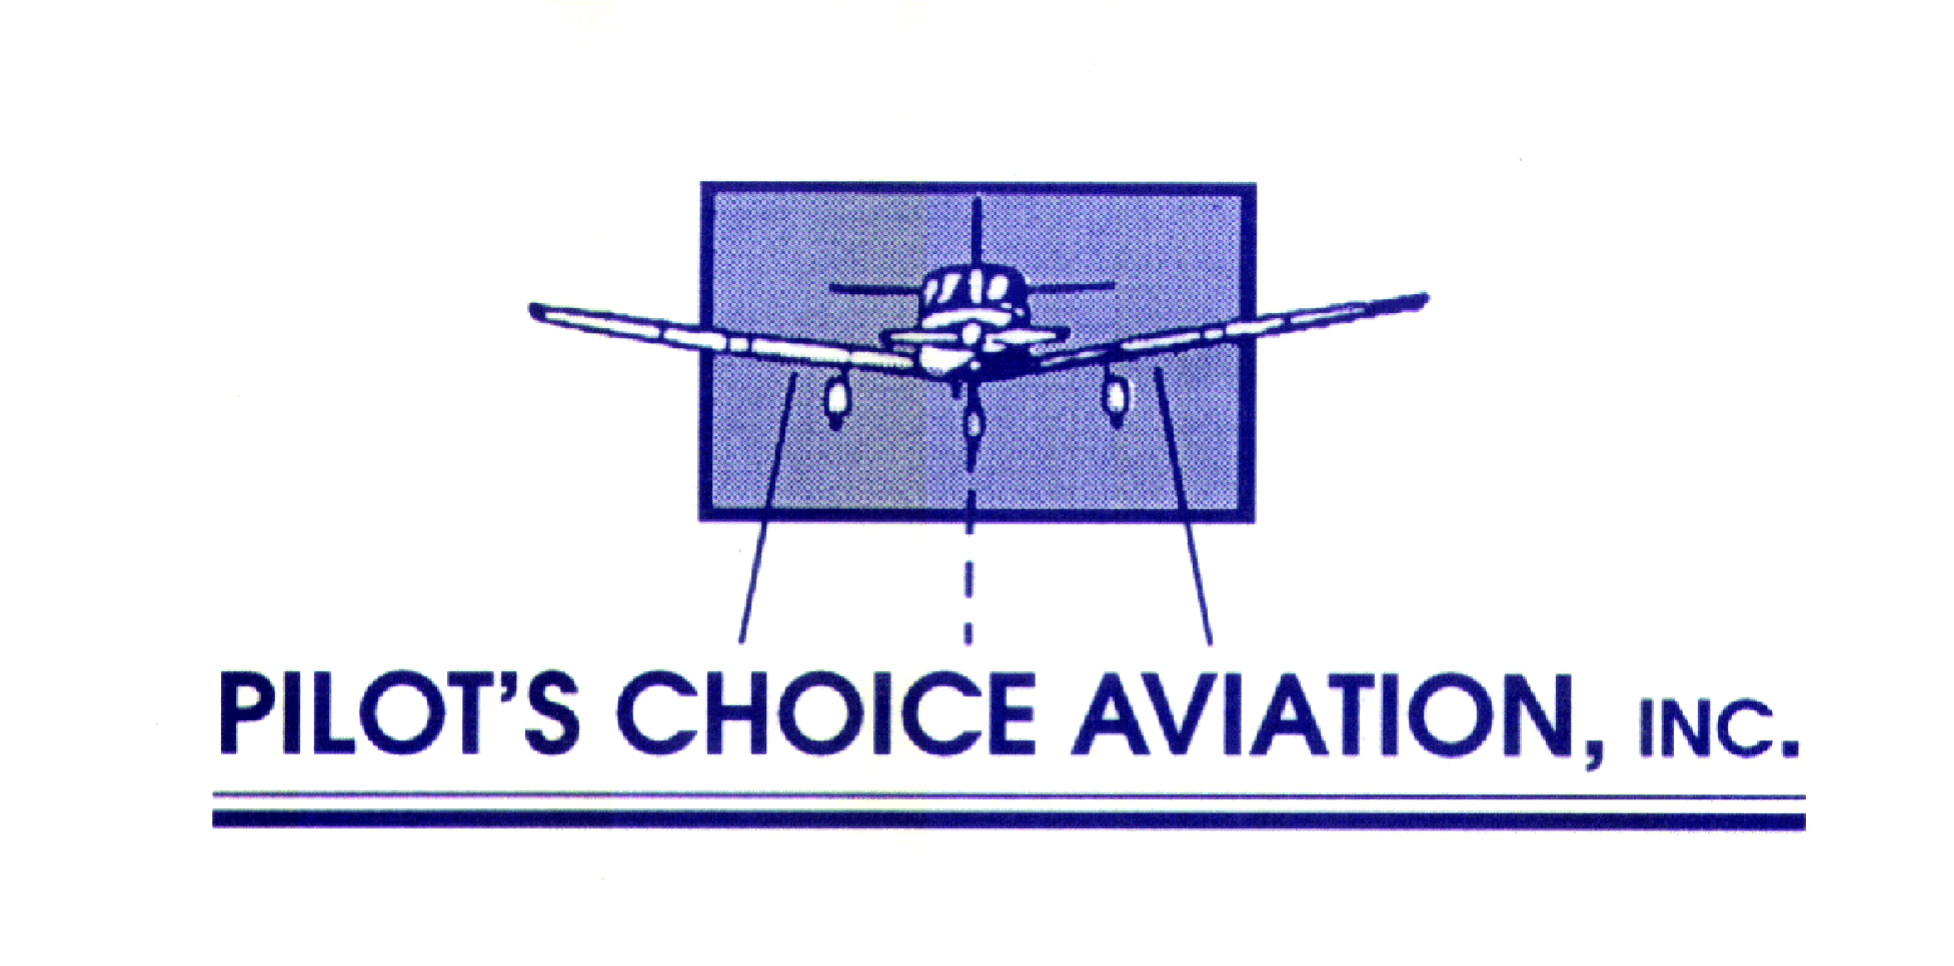
\includegraphics[width=0.9\linewidth]{pca-logo}
\end{center}

Do you want to fly the ``big iron''? Are you looking for more performance, capability,
and reliability? Do you enjoy engine management (and maintenance) so much that you want to
double the fun? Do you see a type rating in your future? If so, multi engine airplane training is for you.

This Manual focuses on the Beechcraft Duchess BE76, the multi engine trainer used at Pilot's
Choice Aviation, Inc. (PCA) at Georgetown, TX (KGTU).

The material in this book is based upon official resources from the FAA, as well as Beechcraft.

Beth Ann Jenkins authored the previos 2017 edition of this Multiengine Manual. Stephanie Fernihough
added numerous notes and edits from test flying and working with students.

Jos\'e reformatted the Multiengine Manual \LaTeX{} in Spring of 2025. At that time, it was also
updated to include notes eight years of students successfully using this document to become multi
engine pilots. System diagrams were upgraded to new, higher quality vector graphics. This Manual
contains updated material the latest FAA ACS testing documents as of this writing.

\newpage

\section*{Disclaimer}

The information contained in this publication is subject to change.

Aeronautical information, regulations, and aircraft information change regularly, therefore those relevant
publications should be referred to for any critical information.

The information in this manual is to be utilized for training purposes only. Always
refer to your aircraft's POH, AFM, and other certified documentation before flight!

\chapter{Single Engine Aerodymanics}

%Keep it above \vyse or bad things happen.
%Keep it above \vmc or really bad things happen.

With a few exceptions, flying a multiengine airplane in normal operations is similar to flying a
complex single. Most of the differences between single-engine and multi-engine flying relate to
emergency situations. Specifically, we are concerned with the airplane’s flight characteristics
when only one engine is fully operating.

The discussion to follow will focus on two key elements of multi-engine flying: performance and controllability.

Note: \emph{performance} and \emph{controllability} are complementary. As one increases, the other decreases, and vice versa.

\section{The Engine-Inoperative Condition}

\subsection{Asymmetric Thrust}

Engines on conventional twins are mounted on the wings. Unlike a single-engine airplane, the engine thrust is not
directed along the longitudinal axis of the airplane. Rather, each engine’s thrust produces a moment that attempts to
yaw the airplane around its vertical axis. On the Duchess (one counter-rotating prop) when both engines are
producing equal thrust, these moments balance each other out and the net thrust has no yawing moment. When one
engine is at reduced or zero thrust, there is a net yawing moment that will lead to a loss of directional control if not
counteracted.

Just like in a single, yawing moments (such as propeller left-turning tendencies in a climb) are counteracted with
rudder. When an engine fails in a multi-engine airplane, the yaw that occurs must be balanced out with enough
rudder pressure to keep the airplane straight. Rudder effectiveness is a function of airspeed – more air flowing over
the rudder airfoil gives it the ability to produce more horizontal lift.

\subsection{Accelerated Slipstream}

Because the engines on a conventional twin are wing-mounted, additional lift is produced by the accelerated
slipstream of the propeller wash over the wing surface. The loss of thrust on one wing results in a loss of lift on that
wing which produces an imbalance of lift between the two wings, leading to a rolling moment toward the
inoperative engine. This rolling tendency must be counteracted with aileron deflection.

\subsection{Summary}

Because of the above listed factors (asymmetric thrust and accelerated slipstream), both produced by the operating
engine, there is a tendency for the airplane to \emph{both} roll \emph{and} yaw into the inoperative engine!

\section{Engine-Inoperative Performance}

\subsection{Loss of Horsepower}

A common misconception is that with one engine out, a twin will have half the climb performance
that it would with both engines. In reality, for aircraft with a maximum gross weight of less than
6,000 pounds, there is no
requirement that they be capable of level flight or climb for \emph{any} weight or flight condition! The only requirement is
that the rate of climb or descent be determined. Many light twins are not capable of holding altitude with one engine.

The Duchess has two 180-HP engines for a total of 360 HP, and requires about 140 HP to maintain level flight.
Losing one engine drastically cuts the horsepower available for climb performance:

\begin{table}[h]
\centering
\begin{tabular}{cl}
\textbf{360}   & \textbf{total HP available}            \\
\textbf{(140)} & \textbf{HP for level flight}           \\ \hline
\textbf{220}   & \textbf{HP left for climb performance} \\
\textbf{(180)} & \textbf{HP -- loss of an engine}       \\ \hline
\textbf{40}    & \textbf{HP now available for climb}
\end{tabular}
\caption{Single engine performance for the Duchess.}
\end{table}

This means we now have only approximately 20\% (40/220) climb performance remaining. In addition,
it should be
stressed that the airplane must be cleaned up to climb. Anything that creates drag will
require additional horsepower
and will decrease the airplane’s climb performance.

Further, realize that 180 HP is the rated horsepower for sea-level standard conditions. Depending on density altitude
(pressure altitude and temperature) effective horsepower may be less than 180 HP. This means that you 
\emph{may not be able to maintain altitude with only one engine}. Maintaining \vyse (blue line) will give you a best rate of climb or the
least rate of descent.

\subsection{\vyse (\textcolor{blue}{Blue Line})}


\vyse is the maximum rate of climb (or minimum rate of sink) airspeed for a single-engine configuration.
It represents
the maximum lift over drag ratio ($L/D_{max}$) with one engine operating, and may be likened to the best glide speed in a
single-engine airplane. At slower airspeeds, induced drag becomes more prominent. At faster speeds, parasite drag
becomes more prominent.

\vyse is the minimum speed to use during all phases of flight and is to be exceeded until committed to land on short
final. \vyse is the minimum speed above which you can commit to a continued takeoff. \vyse is the minimum speed to
use during emergencies involving an engine failure. \vyse is marked by a \textcolor{blue}{Blue Line} on the airspeed indicator (85
KIAS on the Duchess).

\subsection{Drag Factors}

With one engine inoperative, several factors will determine whether or not you'll be able to maintain altitude, climb
or descend. These drag factors increase the horsepower required for level flight, and eat into the excess horsepower
which could be used for climb. All figures are approximate and will vary with density altitude:

\vbox{%
\begin{enumerate}
    \item Not at \vyse -- High or low by 5 knots: \textbf{100 fpm descent}
    \item Gear Down: \textbf{250 fpm descent}
    \item Full Flaps: \textbf{350 fpm descent} (flaps @ 20 = 150 fpm descent)
    \item Critical engine windmilling: \textbf{300 fpm descent}
\end{enumerate}}

Single engine goarounds may be impossible and \textbf{shall not be attempted with flap settings beyond 20 degrees}.

Each twin has a single engine service ceiling and an absolute single engine ceiling:

\begin{itemize}
\item The \textbf{single-engine service ceiling} (Duchess: 6000 ft @ ISA) is the maximum \emph{density altitude} the airplane can sustain a 50 fpm climb with max power on the good engine in the clean configuration.
\item The \textbf{single-engine absolute ceiling} (Duchess: approximately 7800 ft @ ISA) is the maximum \emph{density altitude} the airplane can maintain on one engine with max power in the clean configuration. This is also the altitude where \vyse
and \vxse meet.
\end{itemize}

\subsection{Engine-Inoperative Controllability}

In a single-engine airplane, keeping the aircraft under control (avoiding a stall) is critical. Even if performance is
below that required to maintain level flight, we accept a descent and a controlled landing rather than try to hold off
the descent and get into a stall/spin situation. While stalls are a concern in multi-engine aircraft, another important
consideration is the possible loss of directional control if airspeed is not managed correctly.

With all this in mind, it can be said that the battle for controllability is one between engine and rudder. Anything
that increases the difference in thrust between the two engines will decrease controllability, and anything that makes
the rudder more able to counteract the thrust difference will increase controllability.

\subsection{Critical Engine and Critical Engine Factors}

The critical engine is the engine whose failure most adversely affects the performance and controllability of the
airplane. In general, one of the engines will have a larger yaw moment and the airspeed needs to be higher in order
to balance it out. When the airplane has counter-rotating props (such as the Duchess) there is no critical engine. On
most twins, both propellers rotate clockwise when viewed from the cockpit. On these aircraft, the left engine is
critical. The reasons for this are explained below.

The following discussion assumes a conventional light twin, with two clockwise-rotating propellers. On such
airplanes, the critical engine is the left engine, because the left-turning tendencies of the right engine add to its
asymmetric thrust. The left turning tendencies are discussed below. (PAST)

\subsubsection{P factor}

The descending blade produces more thrust than the ascending blade. The descending blade on the right engine has
a longer moment arm (A2) than on the left engine (A1). This produces greater asymmetric thrust when the right
engine is operating than when the left engine is operating.

\begin{center}
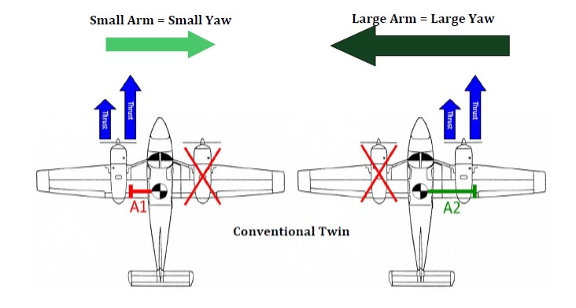
\includegraphics[width=0.9\linewidth]{pfactor}
\end{center}

\subsubsection{Accelerated Slipstream}

The loss of induced airflow created by the propeller over the dead engine wing results in a
loss of lift on that wing. This loss of lift causes a roll towards the dead engine and will
require additional aileron deflection into the operating engine. Due to P-factor, the
accelerated slipstream of the right engine has a longer moment-arm (A2) than the left
engine (A1) because the descending (greater-thrust) propeller blade is outboard.

\begin{center}
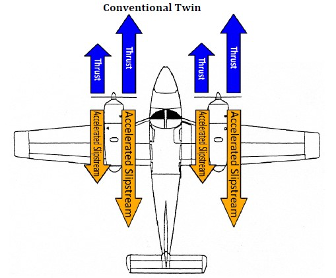
\includegraphics[width=0.5\linewidth]{accel1}
\end{center}

\begin{center}
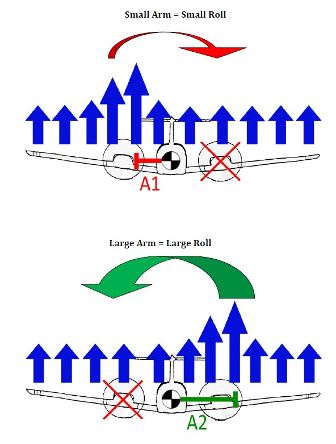
\includegraphics[width=0.5\linewidth]{accel2}
\end{center}

\subsubsection{Spiraling Slipstream}

Both engines produce spiraling slipstreams, but the left engine’s spiraling slipstream is directed towards the rudder, making it more effective. The right engine’s spiraling slipstream is directed away from the rudder. In the event of
left engine failure, the rudder becomes less effective due to the loss of the critical engine’s spiraling slipstream.
Therefore, with critical engine failure maintaining directional control requires more rudder authority.

\begin{center}
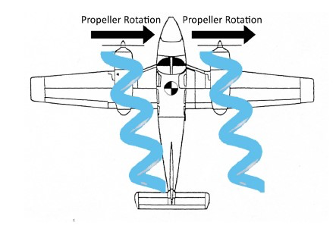
\includegraphics[width=0.5\linewidth]{spiraling}
\end{center}

\subsubsection{Torque}

Torque is the opposite reaction to the clockwise turning of the propellers. Both engines produce a rolling tendency
to the left. With the right engine operating (critical engine inoperative), torque adds to the yaw/roll produced by
asymmetric thrust. With the left engine operating, torque counteracts the yaw/roll produced by asymmetric thrust.

\begin{center}
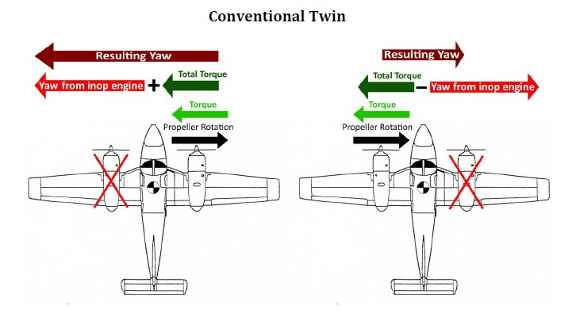
\includegraphics[width=0.9\linewidth]{torque}
\end{center}

\subsection{$V_{MC}$}

\vmc is defined as the minimum speed at which you can maintain directional control
with ithe sudden loss of the critical engine. The actual speed at which you will
lose directional control will vary depending on conditions on a
given day. The \emph{published \vmc airspeed} is dictated by a set of conditions in
14 CFR (FAR) 23.149. \vmc is marked with a \textbf{\textcolor{red}{red line}} on the airspeed indicator.
For the Duchess, this airspeed is \textcolor{red}{65 KIAS}.

On August 30, 2017, a substantial rewrite of 14 CFR (FAR) 23 went into effect. This
rewrite eliminated 23.149 from the current regulations. However, it remains the
certification basis for many of the light piston twin airplanes we fly today. For
light twins certificated under the new Part 23, such as the Tecnam P2006, we would
see similar requirements under 14 CFR (FAR) 23.2xxx. Since this document focuses on
the Duchess, we restrict our discussion to the ``old'' 14 CFR (FAR) 23, which is
archived on ecfr.gov.

\subsection{Determination of $V_{MC}$}

Under the ``old'' 14 CFR Part 23, manufactures of multiengine aircraft were required to demonstrate and publish a \vmc
(minimum control airspeed) under the following specific conditions, which are either set for Standardization (S), or are the Worst Case (W):

\vbox{%
\begin{enumerate}
    \item \textbf{Standard Day} (S) (15\degree C and 29.92" at sea level)
    \item \textbf{Maximum sea level takeoff weight} (S)
    \item \textbf{The most rearward allowable center of gravity} (W)
    \item \textbf{The critical engine failed} (W) and the propeller is
        \begin{enumerate}
            \item Windmilling, or
            \item Feathered, if the aircraft has an auto feather system (rare in light twins)
        \end{enumerate}
    \item \textbf{Takeoff at maximum available power on the good engine} (W)
    \item \textbf{Landing gear up} (W)
    \item \textbf{Flaps in the takeoff position} (S)
    \item \textbf{No more than 5\degree{} of bank into the good engine} (S)
\end{enumerate}}

A further factor is the pilot ability, Part 23 states that recovery from loss of directional
control at \vmc should not require more than average pilot technique and the recovery should
be accomplished within 20\degree{} of original heading.

Apart from the 5\degree{} bank, max gross weight, standard day, and flaps, the remaining factors
are all worst case, and they lead to the highest \vmc to be published by the manufacturer
(65 KIAS for the Duchess), or are related to the takeoff scenario.

When considering \vmc, realize that lower \vmc is better. Anything that lowers \vmc
will increase controllability at lower airspeed, giving more margin for error in
single-engine operation.

\subsubsection{Conditions that the FAA Requires for Published \vmc (14 CFR 23.149)}

What follows is a list of conditions required to be met by manufacturers in
determining the published \vmc value for certification. Understanding the
regulatory criteria is important for understanding how existing conditions and
aircraft control influence single-engine controllability.

The conditions required for certification represent the worst-case scenario
for controllability: an engine failure shortly after takeoff, with the
aircraft in the climb-out configuration. However, not every condition required for
certification is necessarily worst-case (W); some conditions are specified primarily
for standardization purposes (S).

\subsubsection{Standard conditions (ISA: 15\degree C and 29.92” Hg) (Standardization)}

\vmc decreases with increase density altitude. Any condition that decreases
power on the operating engine such as increased altitude, low air density or
high temperature will in turn mean less thrust, which creates less yaw, so \vmc
will decrease. The opposite is also true for any condition that increases power,
such as lower altitude, high density or low temperature, which will increase \vmc.

\emph{Memory aid: Hot = Good}

\subsubsection{Maximum sea-level power on operating engine (Worst case)}

Maximum power on the good engine increases \vmc due to increased asymmetric thrust.

\subsubsection{Critical engine windmilling or auto-feathered if installed (Worst case)}

The windmilling propeller creates drag, which is asymmetric. Therefore, more rudder
authority will be required to offset this asymmetric drag. \vmc is higher
with a windmilling propeller on the inoperative engine.

\subsubsection{Landing gear retracted (Worst case)}

The gear and gear doors extended tend to act like keels on a boat and resist rolling and yawing tendencies by
shifting the center of gravity down the vertical axis of the airplane. Additionally, on a tricycle-gear airplane, the
main gear are located aft of the center of gravity and produce \emph{stabilizing drag} when extended, like a drag chute
would. \vmc is \emph{lower with gear down}.

\subsubsection{Flaps in the takeoff configuration (Standardization)}

A number of considerations determine the relationship between flap setting and \vmc. With flaps extended a lesser
angle of attack is necessary to produce the same amount of lift. Therefore, P-factor is less as well as yaw.
Additionally, flaps increase drag aft of the C.G., providing a stabilizing effect. However, deploying flaps creates
additional lift on the wing with the operating engine since lift increases with the same airspeed. Therefore it is not
straightforward to say that \vmc changes one way or the other with flaps deployed, and this relationship may vary
depending on the airplane.

The Duchess procedures call for flaps fully retracted for takeoff.

\subsubsection{Maximum 5\degree{} bank into good engine (Standardization)}

The maximum bank allowed by the regulations for \vmc determination is five degrees. Any sideslip toward the good
engine increases controllability due to increased rudder effectiveness – the sideslip results in weathervaning
tendencies toward the operating engine. Likewise, sideslip toward the inoperative engine decreases controllability
by introducing a weathervaning moment away from the operating engine. Specifying a maximum of five degrees
limits the manufacturers to a realistic bank angle.

It should be remembered that a bank angle of three degrees towards the good engine with the ball 1/2 off-center
results in minimum drag and maximum climb. Five degrees of bank towards the good engine actually results in a
sideslip toward the good engine, increasing drag but increasing controllability.

\subsubsection{Maximum gross weight (Standardization)}

\vmc is determined at max gross weight. Primarily this is a reference point for standardization purposes.

When the airplane is banked, a sideslip occurs because a component of weight is acting along the wing (similar to
the idea of a wing-down crosswind approach). The spanwise component of weight and sideslip is greater at a higher
weight than a lower weight. Because of this, when the airplane is banked into the operative engine beyond the
zero-sideslip angle, \vmc increases with the decrease in weight, and vice versa.

\emph{Memory aid: Weight increases side slip effectiveness and lowers \vmc.}

\subsubsection{Most adverse CG (usually aft legal CG limit) (Worst case)}

As the CG moves aft, the moment arm between the rudder and C.G. is shortened, producing less leverage for the
rudder. The further aft the C.G., the more rudder authority is required to offset the asymmetric thrust, requiring
greater airspeed. \vmc is higher with an aft C.G.

\subsubsection{Ground effect negligible (Worst case)}

In ground effect there is a reduction in induced drag, so if an engine failure should occur while in ground effect a
lower than normal angle of attack would be required to create the same amount of lift as when out of ground effect.
A lower angle of attack would decrease the effect of P-factor, reduce yaw, and lower \vmc. Operating out of ground
effect results in a higher \vmc than in ground effect.

\begin{center}
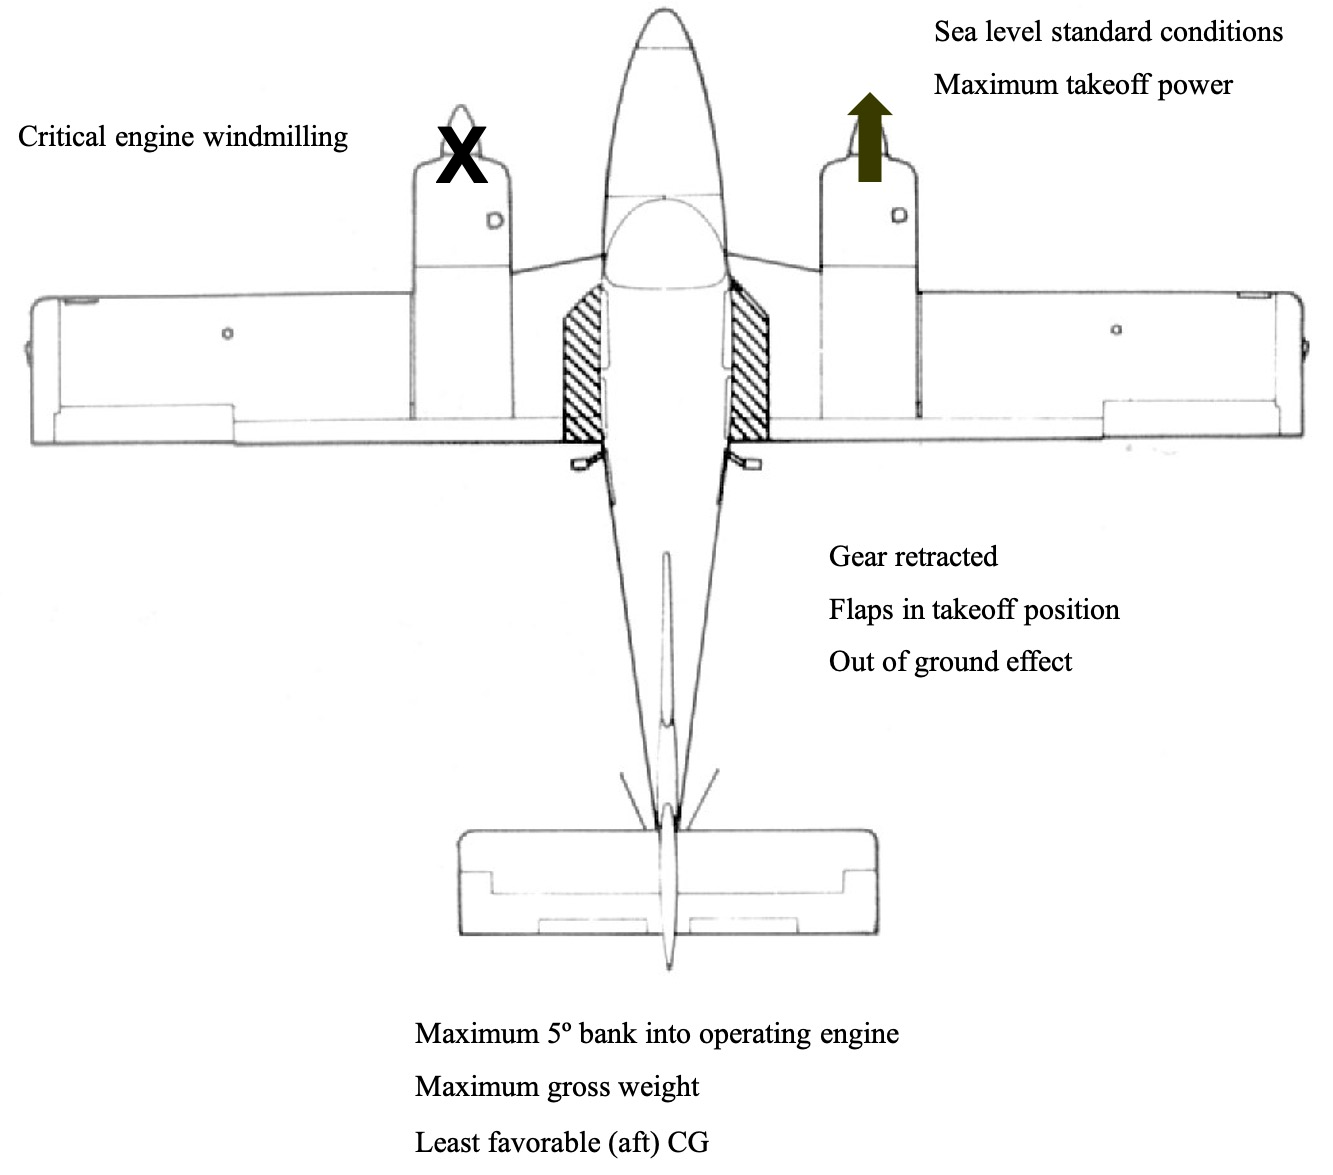
\includegraphics[width=0.9\linewidth]{vmc-conditions}
\end{center}

\emph{Memory aid: Any increase in yaw or decrease in rudder authority \textbf{increases} \vmc!}

\emph{Memory aid: In the least favorable (aft) CG, the arm to the rudder is reduced, so the rudder is less effective.}

\section{Altitude vs. $V_{MC}$ and Stall Speed}

As density altitude increases, \vmc will decrease due to less power output from the operating engine (you'll lose
directional control at a slower airspeed). Indicated stall speed remains relatively constant for all density altitudes.
Thus, it is easily possible for \vmc to be lower than stall speed. When this happens a possible spin could develop
during \vmc demonstrations or during other single-engine operation, real or simulated.

If loss of directional control occurs during single-engine operation, \textbf{IMMEDIATELY} reduce power on the good
engine and lower the nose to regain airspeed.

\begin{center}
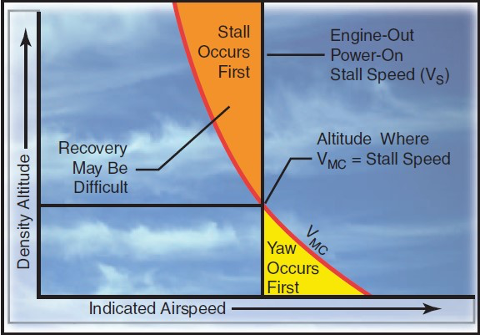
\includegraphics[width=0.8\linewidth]{vmc-stall}
\end{center}

\section{The Zero-Sideslip Condition}

As previously stated, a twin with only one engine operating must counteract the yaw and roll produced by
asymmetric thrust with rudder and aileron. The asymmetric thrust and the \textbf{horizontal lift} produced by the rudder
result in a net sideslip toward the \textbf{inoperative} engine when the wings of the airplane are held level,
causing a turn \emph{away} from the operating engine. This sideslip increases drag and degrades performance
just as a sideslip would in a single.

To overcome this sideslip, the airplane must be banked into the operative engine. The sideslip caused by the bank
angle and ball half-centered cancels out the sideslip created by the engine and rudder resulting in a
\textbf{zero-sideslip condition}. The zero-sideslip condition reduces
drag and therefore improves climb performance (or minimizes rate
of descent). In the Duchess, the bank angle that results in zero sideslip is approximately three degrees.

\begin{center}
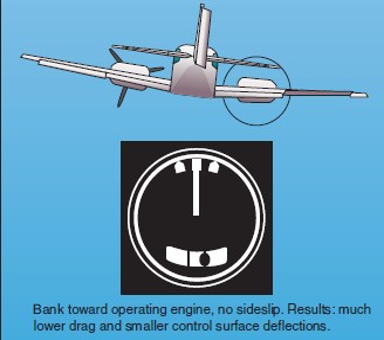
\includegraphics[width=0.6\linewidth]{zero-sideslip}
\end{center}

\emph{Memory aid: Heavier means good engine is less effective, which reduces \vmc.}

\emph{Memory aid: Tail induces centripetal force which turns the airplane. So, you have to counteract that turn
with a bank angle of \emph{3\degree}}.

\chapter{Limitations}

\section{Duchess Speeds}


\begin{table}[h]
\centering
\begin{tabular}{lll}
\textcolor{red}{\textbf{$V_{MC}$}}      & \textbf{65}      & Minimum control speed.                                           \\
\textbf{$V_{S0}$}                       & \textbf{60}      & Stall: landing configuration.                                    \\
\textbf{$V_{S1}$}                       & \textbf{70}      & Stall: clean configuration.                                      \\
\textbf{$V_{XSE}$}                      & \textbf{85}      & Best rate of climb, one engine.                                  \\
\textcolor{blue}{\textbf{$V_{YSE}$}}    & \textbf{85}      & Best angle of climb, one engine.                                 \\ \hline
\multicolumn{1}{|l}{\textbf{$V_{SSE}$}} & \textbf{71}      & \multicolumn{1}{l|}{Intentional one engine inoperative speed.}   \\ \hline
\textbf{$V_A$}                          & \textbf{132}     & Maneuvering speed (at Max gross weight).                         \\
\textbf{$V_{LO}$}                       & \textbf{140/112} & Landing gear operating extend/retract.                           \\
\textbf{$V_{LE}$}                       & \textbf{140}     & Max landing gear extended.                                       \\
\textbf{$V_{FE}$}                       & \textbf{120/110} & Max flaps extended 20/35.                                        \\
\textbf{$V_{NO}$}                       & \textbf{154}     & Max structural cruising speed.                                   \\
\textbf{$V_{NE}$}                       & \textbf{194}     & Never exceed speed.                                              \\
\textbf{$V_R$}                          & \textbf{71}      & Rotation speed. For training purposes, $V_R$ is increased to 80. \\
\textbf{$V_X$}                          & \textbf{71}      & Best angle of climb.                                             \\
\textbf{$V_Y$}                          & \textbf{85}      & Best rate of climb.                                              \\
\textbf{}                               & \textbf{140}     & Emergency descent. \emph{Do not exceed!}                         \\
\textbf{}                               & \textbf{100}     & Emergency landing gear extension (free fall), maximum.           \\
\textbf{}                               & \textbf{95}      & Best glide: 12:1 with propellers feathered.                      \\
\textbf{}                               & \textbf{25}      & Maximum demonstrated crosswind component.
\end{tabular}
\end{table}

\section{Weight Limits}

\begin{table}[h]
\centering
\begin{tabular}{ll}
\textbf{Maximum Ramp Weight}              & 3916 Pounds \\
\textbf{Maximum Takeoff Weight}           & 3900 Pounds \\
\textbf{Maximum Landing Weight}           & 3900 Pounds \\
\textbf{Maximum Zero Fuel Weight}         & 3500 Pounds \\
\textbf{Maximum Baggage Compartment Load} & 200 Pounds 
\end{tabular}
\end{table}

\chapter{Emergency Procedures}

\textbf{KNOW PROCEDURES BY MEMORY!}

\section{Engine Failure in Flight (above 3000' AGL)}

\subsection{Procedures}

\textbf{Maintain directional control!}

\textbf{ALL AVAILABLE POWER:}
\begin{enumerate}
    \item \textbf{PITCH FOR \textcolor{blue}{BLUE LINE} - \vyse (85 KIAS),\\OR maintain altitude at a higher airspeed if able.}
    \item \textbf{\textcolor{red}{MIXTURES} SET (max available power)}
    \item \textbf{\textcolor{blue}{PROPELLERS} Full Forward}
    \item \textbf{THROTTLES Full Power}
\end{enumerate}

\textbf{CLEAN UP:}
\begin{enumerate}
    \item \textbf{FLAPS UP (or as required)}
    \item \textbf{GEAR UP (or as required)}
    \item \textbf{Trim and bank into good engine.}
\end{enumerate}

\textbf{IDENTIFY/VERIFY:}
\begin{enumerate}
    \item \textbf{IDENTIFY Dead foot = dead engine.}
    \item \textbf{VERIFY Power idle on dead engine. No change in performance - verified.}
\end{enumerate}

\textbf{FIX OR FEATHER:}
\begin{itemize}
    \item \textbf{DECISION Based upon situation/altitude (Restart or Feather?)}
\end{itemize}

Rarely do engines fail suddenly and completely (fuel starvation is the exception). If an engine is running poorly, but
developing some power, \textbf{you are better off letting it run} (above 3000 AGL) until you sort out the problem. The
decision to feather should be made with some deliberation. A catastrophic engine failure would require feathering
the engine (avoiding a potential fire), however, a rough running engine should not be feathered as any horsepower it
is producing potentially helps.

\textbf{The exception is during a critical phase of flight}, such as initial climb-out,
approach or landing. During these phases of flight the propeller on the problem engine should be feathered
immediately, as there is not enough time to safely perform the fix procedures. Maintaining aircraft control is
\emph{the priority} and you should land as soon and as safely as possible.

\textbf{FIX:}

\textbf{CHECK (\textcolor{red}{Red Items}) - only on affected engine.}
\begin{enumerate}
    \item \textbf{Fuel - ON}
    \item \textbf{Carburetor Heat - ON}
    \item \textbf{Mixture - SET (max available power)}
    \item \textbf{Boost Pumps - ON}
    \item \textbf{Magnetos - CYCLE Left - Right - Both}
\end{enumerate}

\textbf{\textcolor{red}{WARNING} Feathering the wrong engine is incredibly dangerous!
Work methodically to make certain the correct engine is feathered.}

\textbf{FEATHER:}
\begin{enumerate}
    \item \textbf{Feather Propeller on inoperative engine.}
    \item \textbf{Power as needed on good engine to maintain altitude/airspeed.\\Minimum speed: \textcolor{blue}{BLUE LINE 85 KIAS}.}
\end{enumerate}

\emph{Memory aid: 3\degree{} bank for slip.}

\textbf{SHUTDOWN AND SECURE ENGINE:}
\begin{itemize}
    \item \textbf{Mixture - Idle Cutoff}
    \item \textbf{Fuel Selector - OFF}
    \item \textbf{Cowl Flaps - Open on operative engine, closed on inoperative engine.}
    \item \textbf{Fuel Pump - OFF}
    \item \textbf{Magnetos - OFF}
    \item \textbf{Alternator Switch - OFF}
    \item \textbf{Notify ATC.}
    \item \textbf{Land as soon as practical.}
\end{itemize}

\textbf{\textcolor{red}{** NOW REFER TO CHECKLIST. **}}


\section{Engine Failure During or After Takeoff}

\subsection{Procedures}

{\centering
\textbf{DURING INITIAL CLIMB OUT THE NOSE NEEDS TO BE LOWERED\\
5 DEGREES OR MORE TO MAINTAIN 85 KIAS!!!}
\par }

Bank approximately \textbf{3 degrees} toward the good engine with the rudder ball half out toward the good engine. This
will provide maximum climb performance. \textbf{Each degree of bank back toward the inoperative engine increases \vmc
by 3 knots per degree. Therefore, with only a 2 degree bank toward the operative engine, \vmc might be 3 knots higher
than published.}

If the pilot inadvertently or instinctively tries to hold wings level in an engine out situation, \vmc
\textbf{CAN INCREASE AS MUCH AS 15 KNOTS. THE AIRCRAFT COULD BE UNCONTROLLABLE AT A
SPEED AS HIGH AS \vyse!} This situation \textbf{WILL EXIST} if the pilot flies wings level and tries to maintain heading
with the ball centered.

\emph{Memory aid: Raise the dead (engine).}

\subsection{Power-Loss Briefing (Before Takeoff)}

A power loss briefing is to be given before takeoff to remind the pilot of the actions to be taken in the event of a
power loss during or after the takeoff roll. Time is critical so actions must be immediate but deliberate.

\bfseries{

Loss of directional control on the ground:
\begin{itemize}
    \item Throttles - IDLE
    \item Regain Control (mostly rudder)
    \item Brake straight ahead
\end{itemize}

Airborne loss of directional control: usable runway remaining and gear down:
\begin{itemize}
    \item Throttles – IDLE
    \item Land
    \item Brake straight ahead
\end{itemize}

Airborne loss of directional control: no usable runway remaining or gear up:
\begin{itemize}
    \item All available power (maintain Heading and Blue Line):
    \item Clean Up
        \begin{itemize}
            \item[\ding{226}] Flaps – UP
            \item[\ding{226}] Gear – UP
        \end{itemize}
    \item Identify dead engine
    \item Verify dead engine
    \item Feather dead engine
    \item Return for landing
\end{itemize}
%} % \bfseries
\mdseries

\section{Airman Certification Standards}

\emph{Source: FAA-S-ACS-7B, Commercial Pilot for Airplane Category Airman Certification Standards, November 2023} 

\subsection{X.A Maneuvering with One Engine Inoperative (AMEL, AMES)}

% From https://www.tablesgenerator.com/ with modifications for [H] and raggedleft/right.

\begin{table}[H]
\centering
\begin{tabular}%
  {>{\raggedleft\arraybackslash}p{0.15\linewidth}%
   >{\raggedright\arraybackslash}p{0.8\linewidth}%
  }
%\textbf{Task}                                                      & \textbf{A. Maneuvering with One Engine Inoperative (AMEL, AMES)}                                                                                                        \\ \hline
\textit{References:}                                                & \textit{FAA-H-8083-2, FAA-H-8083-3, FAA-H-8083-25; FAA-P-8740-66; POH/AFM}                                                                                              \\
\textbf{Objective:}                                                 & To determine the applicant exhibits satisfactory knowledge, risk management, and skills associated with maneuvering with one engine inoperative.                        \\
\textit{\textbf{Note:}}                                             & \textit{See Appendix 2: Safety of Flight and Appendix 3: Aircraft, Equipment, and Operational Requirements \& Limitations for information related to this Task.}        \\ \hline
\textbf{Knowledge:}                                                 & The applicant demonstrates understanding of:                                                                                                                            \\
\textit{CA.X.A.K1}                                                 & Factors affecting minimum controllable speed (VMC)                                                                                                                      \\
\textit{CA.X.A.K2}                                                 & VMC (red line) and best single-engine rate of climb airspeed (VYSE) (blue line).                                                                                        \\
\textit{CA.X.A.K3}                                                 & How to identify, verify, feather, and secure an inoperative engine.                                                                                                     \\
\textit{CA.X.A.K4}                                                 & Importance of drag reduction, including propeller feathering, gear and flap retraction, the manufacturer's recommended control input and its relation to zero sideslip. \\
\textit{CA.X.A.K5}                                                 & Feathering, securing, unfeathering, and restarting.                                                                                                                     \\ \hline
\textbf{\begin{tabular}[c]{@{}l@{}}Risk\\ Management:\end{tabular}} & The applicant is able to identify, assess, and mitigate risk associated with:                                                                                           \\
\textit{CA.X.A.R1}                                                 & Potential engine failure during flight.                                                                                                                                 \\
\textit{CA.X.A.R2}                                                 & Collision hazards.                                                                                                                                                      \\
\textit{CA.X.A.R3}                                                 & Configuring the airplane.                                                                                                                                               \\
\textit{CA.X.A.R4}                                                 & Low altitude maneuvering, including stall, spin, or controlled flight into terrain (CFIT).                                                                              \\
\textit{CA.X.A.R5}                                                 & Distractions, task prioritization, loss of situational awareness, or disorientation.                                                                                    \\ \hline
\textbf{Skills:}                                                    & The applicant exhibits the skill to:                                                                                                                                    \\
    \textit{CA.X.A.S1}                                                          & Recognize an engine failure, maintain control, use manufacturer’s memory item procedures, and use appropriate emergency procedures.                                     \\
    \textit{CA.X.A.S2}                                                          & Set the engine controls, identify and verify the inoperative engine, and feather the appropriate propeller.                                                             \\
    \textit{CA.X.A.S3}                                                          & Use flight controls in the proper combination as recommended by the manufacturer, or as required to maintain best performance, and trim as required.                    \\
    \textit{CA.X.A.S4}                                                          & Attempt to determine and resolve the reason for the engine failure.                                                                                                     \\
    \textit{CA.X.A.S5}                                                          & Secure the inoperative engine and monitor the operating engine and make necessary adjustments.                                                                          \\
    \textit{CA.X.A.S6}                                                          & Restart the inoperative engine using manufacturer’s restart procedures.                                                                                                 \\
    \textit{CA.X.A.S7}                                                          & Maintain altitude ±100 feet or minimum sink rate if applicable, airspeed ±10 knots, and selected headings ±10°.                                                         \\
    \textit{CA.X.A.S8}                                                          & Complete the appropriate checklist(s).                                                                                                                                 
\end{tabular}
\end{table}
  
% Engine Failure During Takeoff Before VMC (Simulated) (AMEL, AMES)

\newpage

\subsection{IX.E Engine Failure During Takeoff Before VMC (Simulated) (AMEL, AMES)}

\begin{table}[h]
\centering
\begin{tabular}%
  {>{\raggedleft\arraybackslash}p{0.15\linewidth}%
   >{\raggedright\arraybackslash}p{0.8\linewidth}%
  }
\textit{References:}       & \textit{FAA-H-8083-2, FAA-H-8083-3, FAA-H-8083-25; FAA-P-8740-66; POH/AFM}                                                                                                        \\
\textbf{Objective:}        & To determine the applicant exhibits satisfactory knowledge, risk management, and skills associated with engine failure during takeoff before minimum controllable airspeed (VMC). \\
\textit{\textbf{Note:}}    & \textit{See Appendix 2: Safety of Flight and Appendix 3: Aircraft, Equipment, and Operational Requirements \& Limitations for information related to this Task.}                  \\ \hline
\textbf{Knowledge:}        & The applicant demonstrates understanding of:                                                                                                                                      \\
\textit{CA.IX.E.K1}        & Factors affecting minimum controllable speed (VMC).                                                                                                                               \\
\textit{CA.IX.E.K2}        & VMC (red line) and best single-engine rate of climb airspeed (VYSE) (blue line).                                                                                                  \\
\textit{CA.IX.E.K3}        & Accelerate/stop distance.                                                                                                                                                         \\ \hline
\textbf{\begin{tabular}[c]{@{}l@{}}Risk\\ Management:\end{tabular}}  & The applicant is able to identify, assess, and mitigate risk associated with:                                                                                                     \\
\textit{CA.IX.E.R1}        & Potential engine failure during takeoff.                                                                                                                                          \\
\textit{CA.IX.E.R2}        & Configuring the airplane.                                                                                                                                                         \\
\textit{CA.IX.E.R3}        & Distractions, task prioritization, loss of situational awareness, or disorientation.                                                                                              \\ \hline
\textbf{Skills:}           & The applicant exhibits the skill to:                                                                                                                                              \\
\textit{CA.IX.E.S1}        & Close the throttles smoothly and promptly when a simulated engine failure occurs.                                                                                                 \\
\textit{CA.IX.E.S2}        & Maintain directional control and apply brakes (AMEL), or flight controls (AMES), as necessary.                                                                                   
\end{tabular}
\end{table}

\newpage

\subsection{IX.F Engine Failure After Liftoff (Simulated) (AMEL, AMES)}

\begin{table}[H]
\centering
%\begin{tabular}{rl}
\begin{tabular}%
  {>{\raggedleft\arraybackslash}p{0.15\linewidth}%
   >{\raggedright\arraybackslash}p{0.8\linewidth}%
  }
\textit{References:}                                                                    & \textit{FAA-H-8083-2, FAA-H-8083-3, FAA-H-8083-25; FAA-P-8740-66; POH/AFM}                                                                                                                                                 \\
\textbf{Objective:}                                                                     & To determine the applicant exhibits satisfactory knowledge, risk management, and skills associated with engine failure after liftoff.                                                                                      \\
\textit{\textbf{Note:}}                                                                 & \textit{See Appendix 2: Safety of Flight and Appendix 3: Aircraft, Equipment, and Operational Requirements \& Limitations for information related to this Task.}                                                           \\ \hline
\textbf{Knowledge:}                                                                     & The applicant demonstrates understanding of:                                                                                                                                                                               \\
\textit{CA.IX.F.K1}                                                                     & Factors affecting minimum controllable speed (VMC).                                                                                                                                                                        \\
\textit{CA.IX.F.K2}                                                                     & VMC (red line), VYSE (blue line), and safe single-engine speed (VSSE).                                                                                                                                                     \\
\textit{CA.IX.F.K3}                                                                     & Accelerate/stop and accelerate/go distances.                                                                                                                                                                               \\
\textit{CA.IX.F.K4}                                                                     & How to identify, verify, feather, and secure an inoperative engine.                                                                                                                                                        \\
\textit{CA.IX.F.K5}                                                                     & Importance of drag reduction, including propeller feathering, gear and flap retraction, the manufacturer’s recommended control input and its relation to zero sideslip.                                                    \\
\textit{CA.IX.F.K6}                                                                     & Simulated propeller feathering and the evaluator’s zero-thrust procedures and responsibilities.                                                                                                                            \\ \hline
\multicolumn{1}{l}{\textbf{\begin{tabular}[c]{@{}l@{}}Risk\\ Management:\end{tabular}}} & The applicant is able to identify, assess, and mitigate risk associated with:                                                                                                                                              \\
\textit{CA.IX.F.R1}                                                                     & Potential engine failure after lift-off.                                                                                                                                                                                   \\
\textit{CA.IX.F.R2}                                                                     & Collision hazards.                                                                                                                                                                                                         \\
\textit{CA.IX.F.R3}                                                                     & Configuring the airplane.                                                                                                                                                                                                  \\
\textit{CA.IX.F.R4}                                                                     & Low altitude maneuvering, including stall, spin, or controlled flight into terrain (CFIT).                                                                                                                                 \\
\textit{CA.IX.F.R5}                                                                     & Distractions, task prioritization, loss of situational awareness, or disorientation.                                                                                                                                       \\ \hline
\textbf{Skills:}                                                                        & The applicant exhibits the skill to:                                                                                                                                                                                       \\
\textit{CA.IX.F.S1}                                                                     & Promptly recognize an engine failure, maintain control, and use appropriate emergency procedures.                                                                                                                          \\
\textit{CA.IX.F.S2}                                                                     & Establish VYSE; if obstructions are present, establish best single-engine angle of climb speed (VXSE) or VMC +5 knots, whichever is greater, until obstructions are cleared. Then transition to VYSE.                      \\
\textit{CA.IX.F.S3}                                                                     & Reduce drag by retracting landing gear and flaps in accordance with the manufacturer’s guidance.                                                                                                                           \\
\textit{CA.IX.F.S4}                                                                     & Simulate feathering the propeller on the inoperative engine (evaluator should then establish zero thrust on the inoperative engine).                                                                                       \\
\textit{CA.IX.F.S5}                                                                     & Use flight controls in the proper combination as recommended by the manufacturer, or as required to maintain best performance, and trim as required.                                                                       \\
\textit{CA.IX.F.S6}                                                                     & Monitor the operating engine and aircraft systems and make adjustments as necessary.                                                                                                                                       \\
\textit{CA.IX.F.S7}                                                                     & Recognize the airplane’s performance capabilities. If a climb is not possible at VYSE, maintain VYSE and return to the departure airport for landing, or initiate an approach to the most suitable landing area available. \\
\textit{CA.IX.F.S8}                                                                     & Simulate securing the inoperative engine.                                                                                                                                                                                  \\
\textit{CA.IX.F.S9}                                                                     & Maintain heading ±10° and airspeed ±5 knots.                                                                                                                                                                               \\
\textit{CA.IX.F.S10}                                                                    & Complete the appropriate checklist(s).
\end{tabular}
\end{table}

\chapter{Normal Procedures}

Refer to aircraft checklists for detailed procedures. The procedures listed below
should be memorized and chair-flown until familiar.

% vim :set indentexpr=

\section{Takeoff}

\begin{itemize}[label={}]
\item Takeoff briefing – GIVEN (see Emergency Procedures)
\item Taxi into position on the runway for takeoff
\item Brakes – APPLY AND HOLD
\item Throttles – 20 MP
\item Engine Gauges – CHECK IN THE GREEN
\item Brakes – RELEASE
\item Throttles – FULL
\item Airspeed Indicator – CHECK ALIVE
\item Rotate at 80 KIAS
\item Gear Up (when positive rate of climb)
\item Climb at 90 KIAS
\end{itemize}

\section{Climb}
\textbf{At 500' AGL:}
\begin{itemize}[label={}]
\item Throttles – 25” MP
\item Propellers – 2500 RPM
\item Cruise climb at 100 KIAS
\item Turn Crosswind or Depart, as Required
\end{itemize}
\textbf{If staying in the pattern, at pattern altitude:}
\begin{itemize}[label={}]
\item Throttles – 20” MP
\item Propellers – 2400 RPM
\end{itemize}

\section{Approach to Landing}
\textbf{Before reaching midfield:}
\begin{itemize}[label={}]
\item Power – 20” MP / 2400 RPM or as required for 100 KIAS
\item Gas: Fuel Selectors – ON; Aux Pumps – ON
\item Undercarriage – DOWN BELOW 140 KIAS
\item Mixtures – SET (max available power)
\item Propellers – 2400 UNTIL FINAL
\item Cowl Flaps – CLOSED
\item Seat Belts – FASTENED
\end{itemize}

\textbf{Abeam the numbers:}
\begin{itemize}[label={}]
\item Throttles – 15” MP
\item Flaps – ID, VERIFY, 10 DEGREES (3 SEC.)
\item Pitch – HALF GROUND / HALF SKY
\item Airspeed – 100 KIAS
\end{itemize}

\textbf{Base leg:}
\begin{itemize}[label={}]
\item Gear Indicators – 3 GREEN
\item Flaps – ID, VERIFY, 20 DEGREES (2 SEC.)
\item Airspeed – 95 KIAS
\item Power – AS REQUIRED
\end{itemize}

\textbf{On final approach (left-to-right flow check):}
\begin{itemize}[label={}]
\item Gear Indicators – 3 GREEN
\item Propellers – FULL FORWARD
\item Mixtures – FULL FORWARD
\item Flaps – FULL (DN)
\item Windsock – CHECK
\item Airspeed – 85 UNTIL SHORT FINAL
\end{itemize}

\textbf{Over the threshold –} CONFIRM 3 GREEN

\section{Touch and Go}

\textbf{Touch and go landings are to be performed only with a Pilot’s Choice Instructor!}

\textbf{On the runway:}
\begin{itemize}[label={}]
\item Flaps – IDENTIFIED (wait for instructor to call VERIFIED) and RETRACTED
\item Cowl Flaps – OPENED
\item Throttles – ADVANCE FOR TAKEOFF \emph{All Available Power}
\end{itemize}

\section{Go-Around}


\begin{itemize}[label={}]
\item \textbf{CRAM} Power - FULL \emph{All Available Power}
\item \textbf{CLIMB} Climb at 85 KIAS (\vyse)
\item \textbf{CLEAN} Flaps – RETRACT ABOVE 71 KIAS
\item \textbf{............} Landing Gear – RETRACT AT 85 AND POSITIVE RATE OF CLIMB
\item \textbf{COOL} Cowl Flaps - OPEN
\item \textbf{CALL} Intentions - ANNOUNCE
\end{itemize}

\newpage

\section{VFR Approach Airspeeds and Power Settings}

\subsection{Traffic Pattern}


% Please add the following required packages to your document preamble:
% \usepackage[normalem]{ulem}
% \useunder{\uline}{\ul}{}
\begin{table}[H]
\begin{tabular}{llll}
              & {\ul Airspeed} & {\ul MP/RPM}             & {\ul Flaps/Configuration}      \\
DOWNWIND      & \textbf{110}   & \textbf{20”/2400}        & \textbf{0}                     \\
Abeam NUMBERS & \textbf{100}   & \textbf{15”/2400}        & \textbf{10\degree{} (3 seconds)}       \\
BASE          & \textbf{100}   & \textbf{15”/2400}        & \textbf{20\degree{} (2 seconds)}       \\
FINAL         & \textbf{90}    & \textbf{12-15”/High RPM} & \textbf{Full flaps (optional)} \\
Over NUMBERS  & \textbf{85}    & \textbf{12-15”/High RPM} & \textbf{Full flaps (optional)}
\end{tabular}
\end{table}


\subsection{Take Off and Climb Out}

% Please add the following required packages to your document preamble:
% \usepackage[normalem]{ulem}
% \useunder{\uline}{\ul}{}
\begin{table}[H]
\begin{tabular}{llll}
         & {\ul Airspeed}              & {\ul MP/RPM}          & {\ul Flaps/Configuration}                       \\
ROTATION & \textbf{80}                 & \textbf{Max/High RPM} & \textbf{0}                                      \\
CLIMB    & \textbf{90 (\vyse or faster)} & \textbf{25”/2500}     & \textbf{0 / Gear up:}     \\
         &                             &                       & \textbf{positive rate, no runway.}
\end{tabular}
\end{table}

\subsection{\textcolor{red}{Single-Engine Pattern}}

% Please add the following required packages to your document preamble:
% \usepackage[normalem]{ulem}
% \useunder{\uline}{\ul}{}
\begin{table}[H]
\begin{tabular}{llll}
         & {\ul Airspeed} & {\ul MP/RPM}              & {\ul Flaps/Configuration}   \\
DOWNWIND & \textbf{\textcolor{blue}{85+}}   & \textbf{As Required/2600} & \textbf{None.}              \\
NUMBERS  & \textbf{\textcolor{blue}{85+}}   & \textbf{20”/2600}         & \textbf{As Required.}       \\
BASE     & \textbf{\textcolor{blue}{85+}}   & \textbf{17-20”/2600}      & \textbf{As Required.}       \\
FINAL    & \textbf{\textcolor{blue}{85}}    & \textbf{Reduce/2600}      & \textbf{20º (for training)}
\end{tabular}
\end{table}

{\centering
\textbf{\textcolor{red}{*GEAR \& FLAPS DOWN \underline{ONLY} WHEN LANDING IS ASSURED!}}
\par }


{\centering
\emph{\textcolor{red}{Memory aid: Gear Mandatory - Do Early. Flaps Optional - Do Late.}}
\par }


\begin{large}

{\centering
\textbf{\textcolor{red}{WARNING!}}
\par }

{\centering
\textbf{\textcolor{red}{\underline{DO NOT} ATTEMPT A ONE-ENGINE INOPERATIVE GO-AROUND AFTER FLAPS HAVE BEEN \underline{FULLY} EXTENDED!}}
\par }

\end{large}

\newpage

\section{Instrument Approach Procedures}

\emph{Memory aid: Recall that VSI depends on ground speed.}

\subsection{Precision Approach, Two Engines}

% Please add the following required packages to your document preamble:
% \usepackage[normalem]{ulem}
% \useunder{\uline}{\ul}{}
\begin{table}[H]
\begin{tabular}%
  {>{\raggedright\arraybackslash}p{0.1\linewidth}%
   >{\raggedright\arraybackslash}p{0.25\linewidth}%
   >{\raggedright\arraybackslash}p{0.4\linewidth}%
   >{\raggedright\arraybackslash}p{0.1\linewidth}%
  }
{\ul Airspeed} & {\ul MP/RPM}      & {\ul Configuration}              & {\ul VSI}     \\
\textbf{110}   & \textbf{18”/2400} & \textbf{Gear down @ Glide slope} & \textbf{-500}
\end{tabular}
\end{table}

\subsection{Precision Approach, Single Engine}

% Please add the following required packages to your document preamble:
% \usepackage[normalem]{ulem}
% \useunder{\uline}{\ul}{}
\begin{table}[H]
\begin{tabular}%
  {>{\raggedright\arraybackslash}p{0.1\linewidth}%
   >{\raggedright\arraybackslash}p{0.25\linewidth}%
   >{\raggedright\arraybackslash}p{0.4\linewidth}%
   >{\raggedright\arraybackslash}p{0.1\linewidth}%
  }
{\ul Airspeed} & {\ul MP/RPM}      & {\ul Configuration}              & {\ul VSI}     \\
\textbf{110}   & \textbf{23”/2500} & \textbf{Gear down @ Glide slope} & \textbf{-500}
\end{tabular}
\end{table}

\subsection{Non-Precision Approach, Two Engines}

% Please add the following required packages to your document preamble:
% \usepackage[normalem]{ulem}
% \useunder{\uline}{\ul}{}
\begin{table}[H]
\begin{tabular}%
  {>{\raggedright\arraybackslash}p{0.1\linewidth}%
   >{\raggedright\arraybackslash}p{0.25\linewidth}%
   >{\raggedright\arraybackslash}p{0.4\linewidth}%
   >{\raggedright\arraybackslash}p{0.1\linewidth}%
  }
{\ul Airspeed} & {\ul MP/RPM}            & {\ul Configuration}      & {\ul VSI}      \\
\textbf{110}   & \textbf{15”/2400 @ FAF} & \textbf{Gear down @ FAF} & \textbf{-1000} \\
\textbf{110}   & \textbf{18”/2400 @ MDA} & \textbf{No change}       & \textbf{0}    
\end{tabular}
\end{table}

\subsection{Non-Precision Approach, Single Engine}

\begin{table}[H]
\begin{tabular}%
  {>{\raggedright\arraybackslash}p{0.1\linewidth}%
   >{\raggedright\arraybackslash}p{0.25\linewidth}%
   >{\raggedright\arraybackslash}p{0.4\linewidth}%
   >{\raggedright\arraybackslash}p{0.1\linewidth}%
  }
{\ul Airspeed} & {\ul MP/RPM}            & {\ul Configuration}                & {\ul VSI}      \\
\textbf{110}   & \textbf{15”/2500 @ FAF} & \textbf{Clean}                     & \textbf{-1000} \\
\textbf{110}   & \textbf{22”/2500 @ MDA} & \textbf{Gear down landing assured} & \textbf{0}    
\end{tabular}
\end{table}

\subsection{Holding Pattern}

\begin{table}[H]
\begin{tabular}%
  {>{\raggedright\arraybackslash}p{0.1\linewidth}%
   >{\raggedright\arraybackslash}p{0.25\linewidth}%
   >{\raggedright\arraybackslash}p{0.4\linewidth}%
   >{\raggedright\arraybackslash}p{0.1\linewidth}%
  }
{\ul Airspeed} & {\ul MP/RPM}      & {\ul Configuration} & {\ul VSI}  \\
\textbf{110}   & \textbf{18”/2400} & \textbf{Clean}      & \textbf{0}
\end{tabular}
\end{table}

\chapter{Performance}


{\centering
\emph{All of the following charts have been included for instructional purposes only.\\Please refer to POH for all calculations of performance.}
\par }

There are two types of charts available for the Duchess that many students are unfamiliar with. A description of these two follows. The rest of the charts are standard.

\section{Accelerate-Stop Distance Defined}

Accelerate-stop distance is the distance required to accelerate to decision speed (71 KIAS for the Duchess) and
brake to a complete stop in the event an engine failure occurs at decision speed. It’s important to realize that
accelerate-stop speed is determined by factory test pilots with prior knowledge of where the failure is to occur.
Therefore, the distances given in the performance charts should be considered the absolute best-case scenario.

\section{Accelerate-Go Distance Defined}

Accelerate-go distance is the distance required to accelerate to decision speed (71 KIAS for the Duchess) and to
continue the takeoff and clear a 50 FT obstacle in the event an engine failure occurs at decision speed. An
accelerate-go distance is only applicable if the airplane can get airborne under the prevailing conditions (weight,
density altitude); single-engine climb performance may not be possible with the gear down.

As with accelerate-stop distance, accelerate-go distance figures are determined by factory test pilots with prior
knowledge of where the failure is to occur. Regard the distances given in the performance charts as the absolute
best-case scenario.

\emph{Memory aid: Any weight 3,600 lbs or more is \underline{always} a no-go!
Do an \underline{accelerate-stop} instead.}

\section{Takeoff Distance}

\begin{figure}[H]
\begin{center}
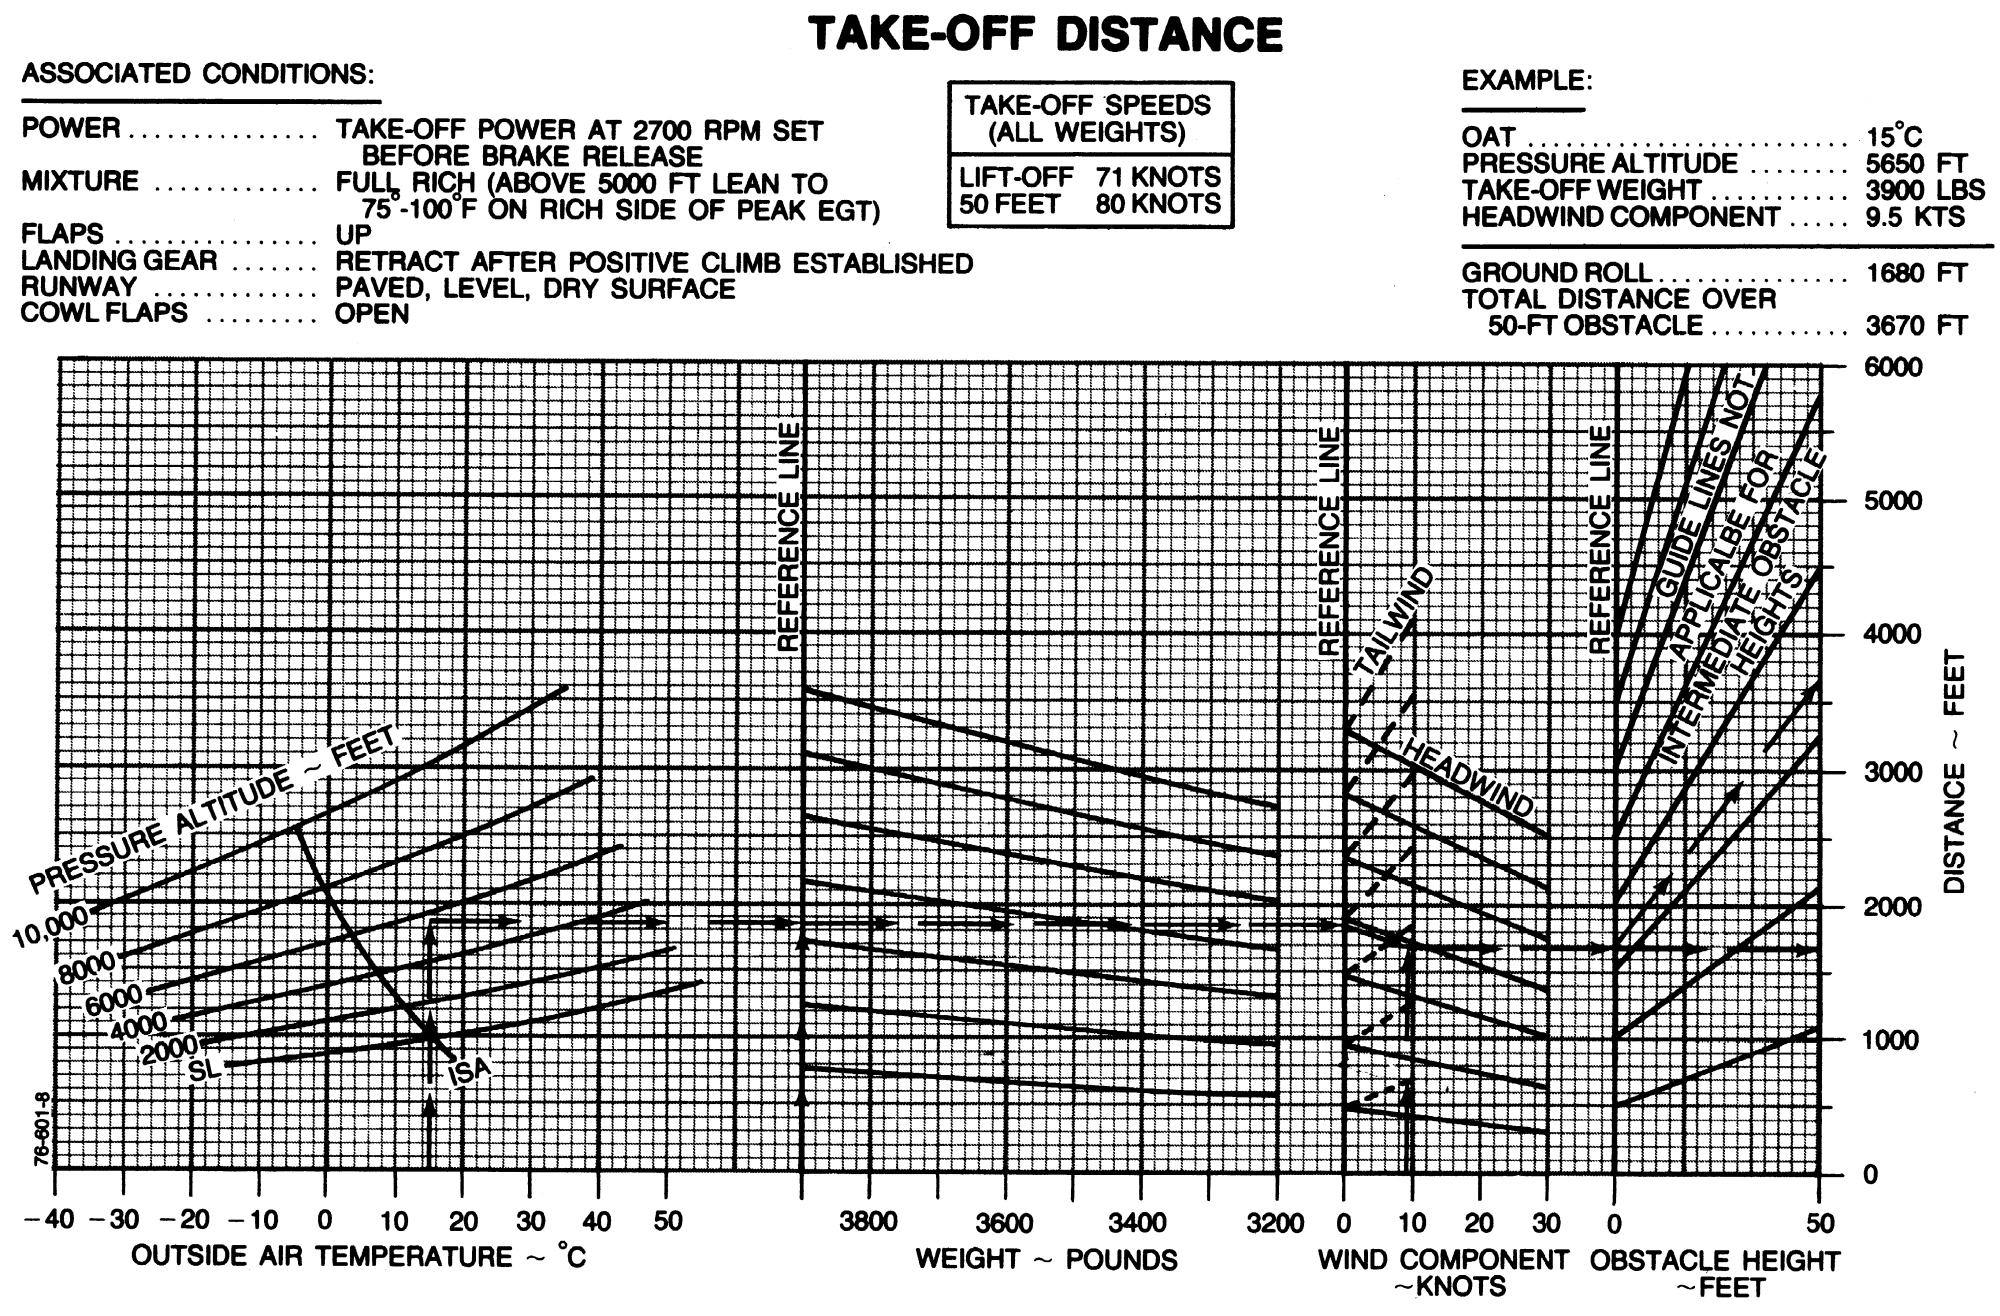
\includegraphics[width=0.95\linewidth]{duchess-takeoff-distance}
\end{center}
\end{figure}

\section{Accelerate-Stop Distance}

\begin{figure}[H]
\begin{center}
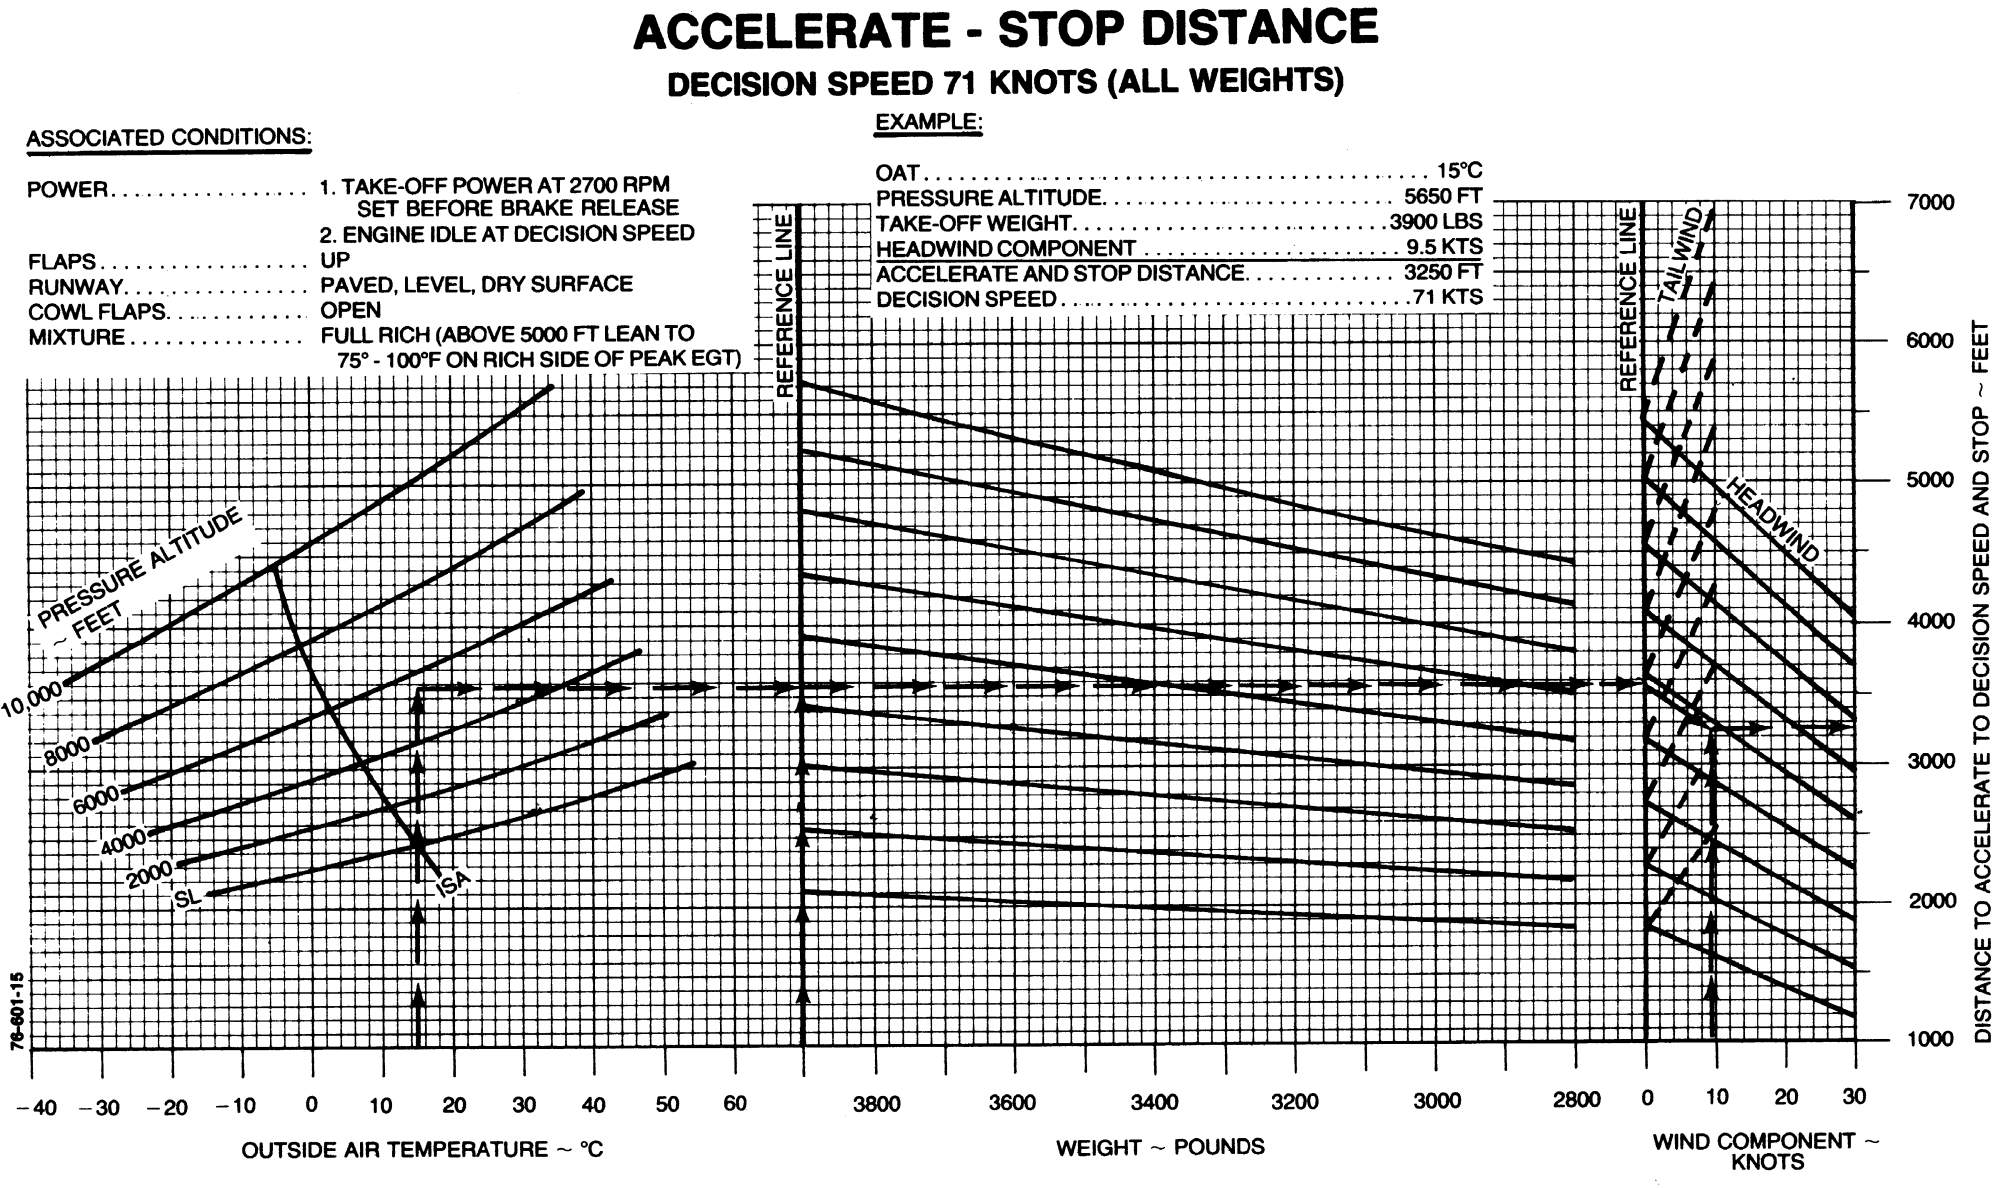
\includegraphics[width=0.95\linewidth]{duchess-asda}
\end{center}
\end{figure}

\section{Accelerate-Go Distance}

\begin{figure}[H]
\begin{center}
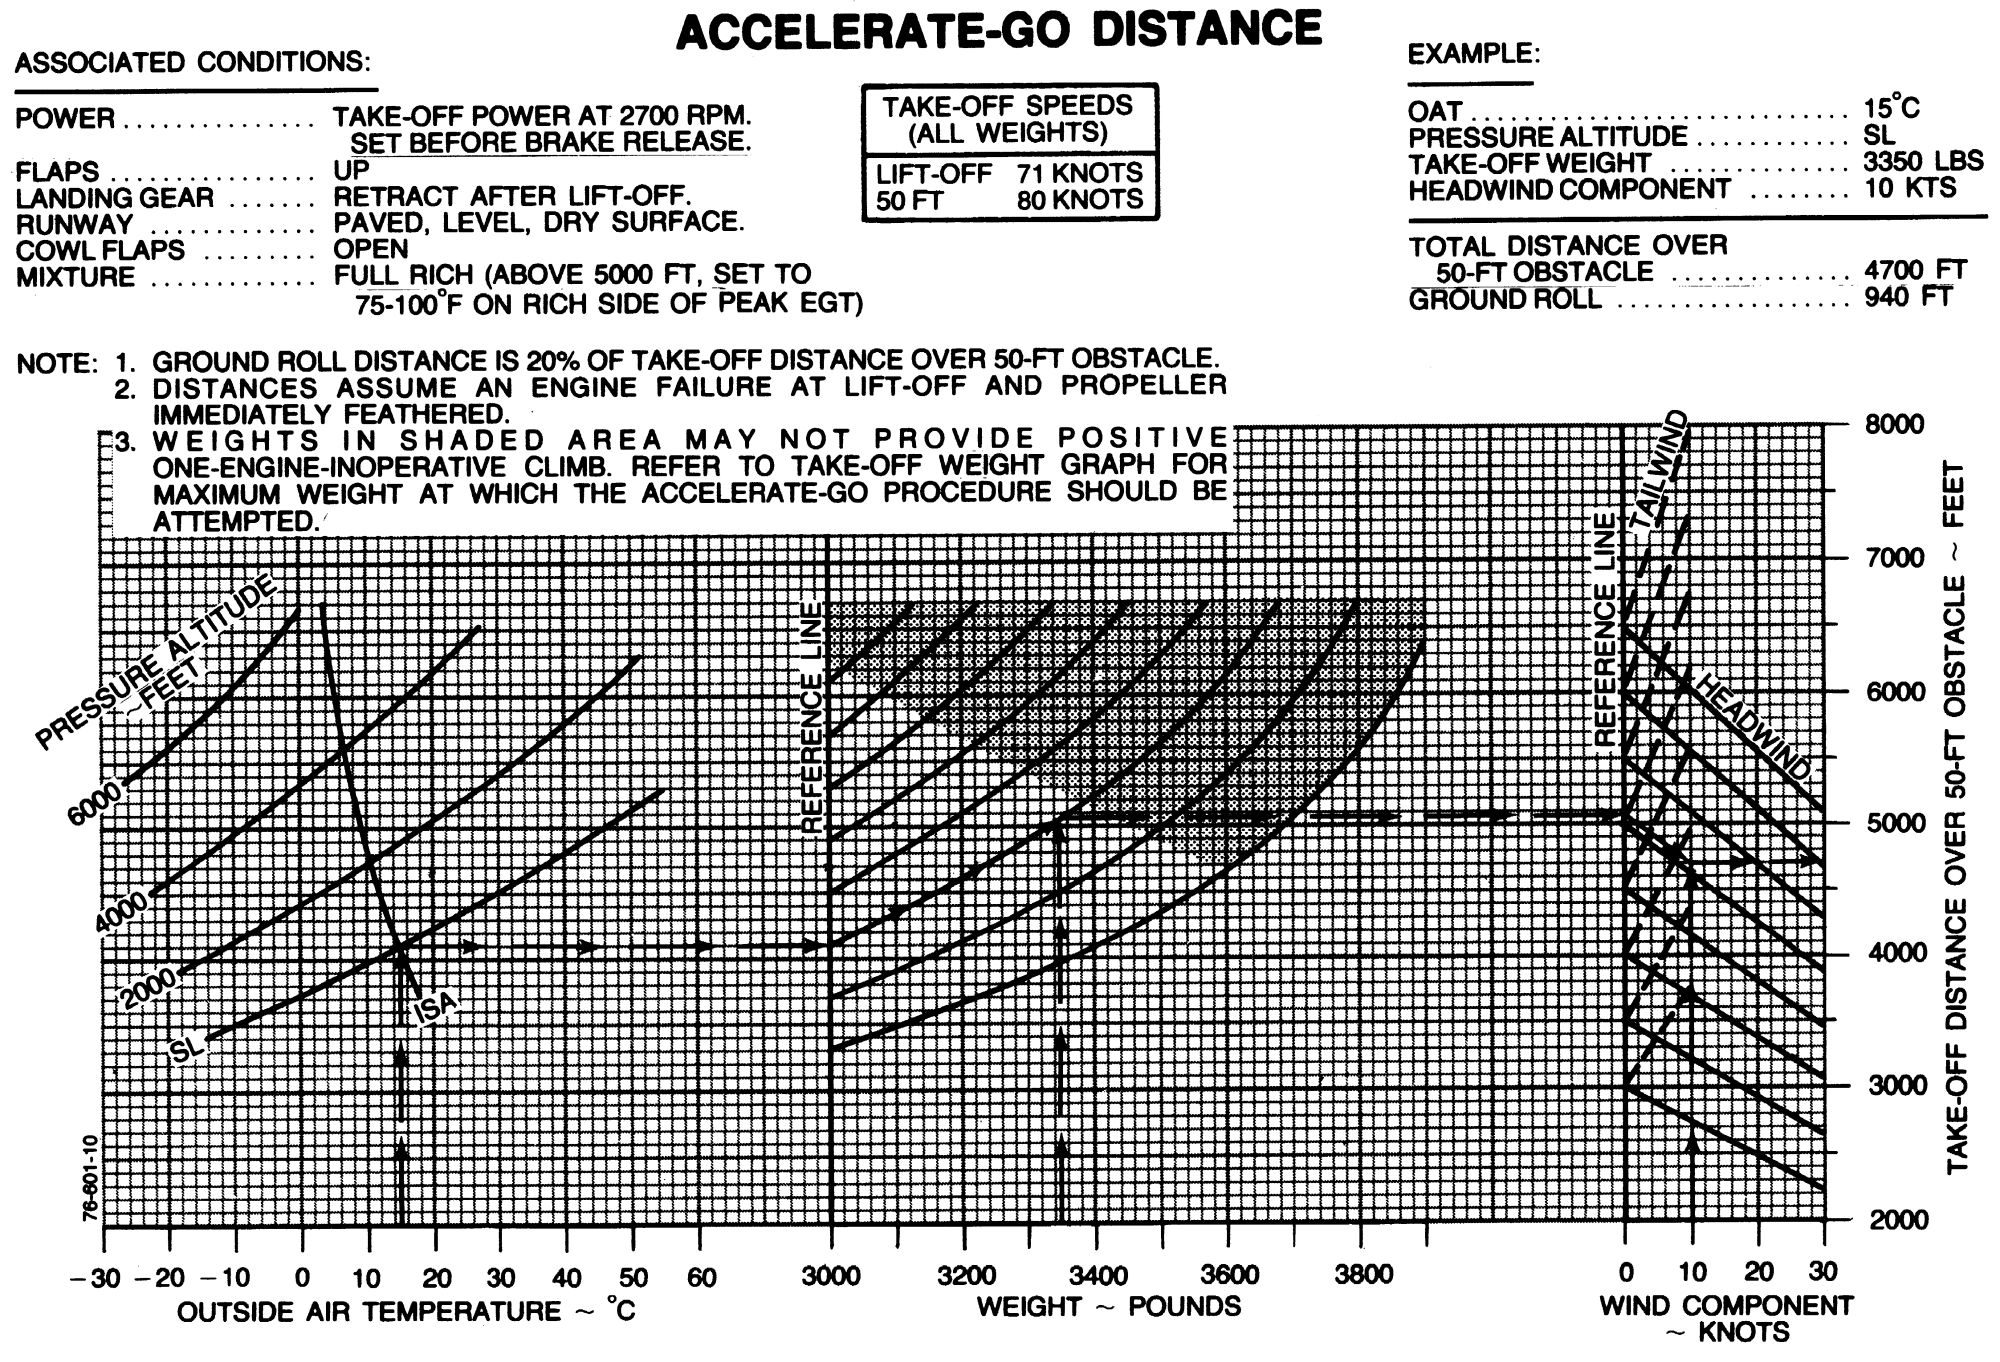
\includegraphics[width=0.95\linewidth]{duchess-accel-go}
\end{center}
\end{figure}

\newpage

\section{Two-Engine Climb Rate}

\begin{figure}[H]
\begin{center}
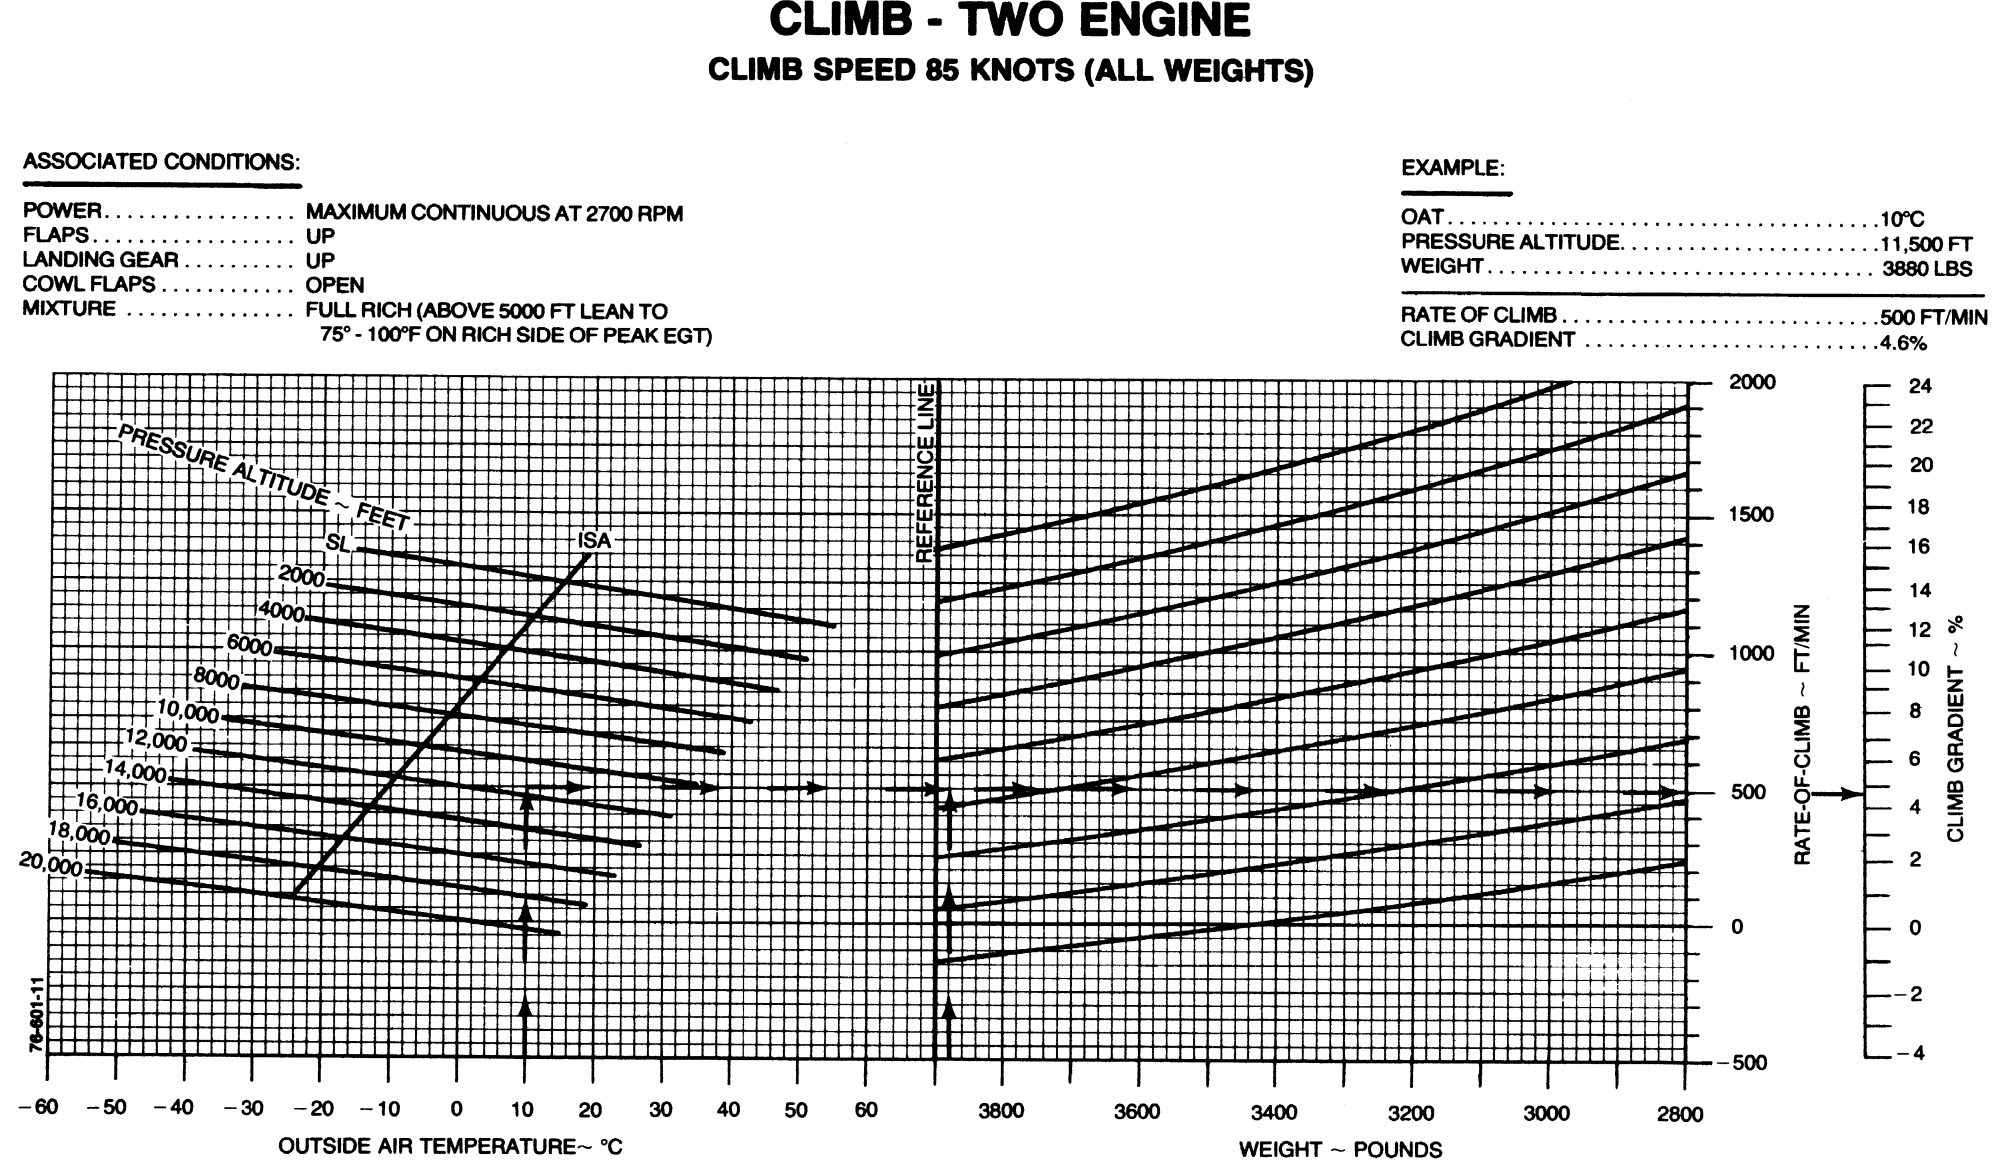
\includegraphics[width=0.9\linewidth]{duchess-2ec}
\end{center}
\end{figure}


\section{Single-Engine Climb Rate}

\begin{figure}[H]
\begin{center}
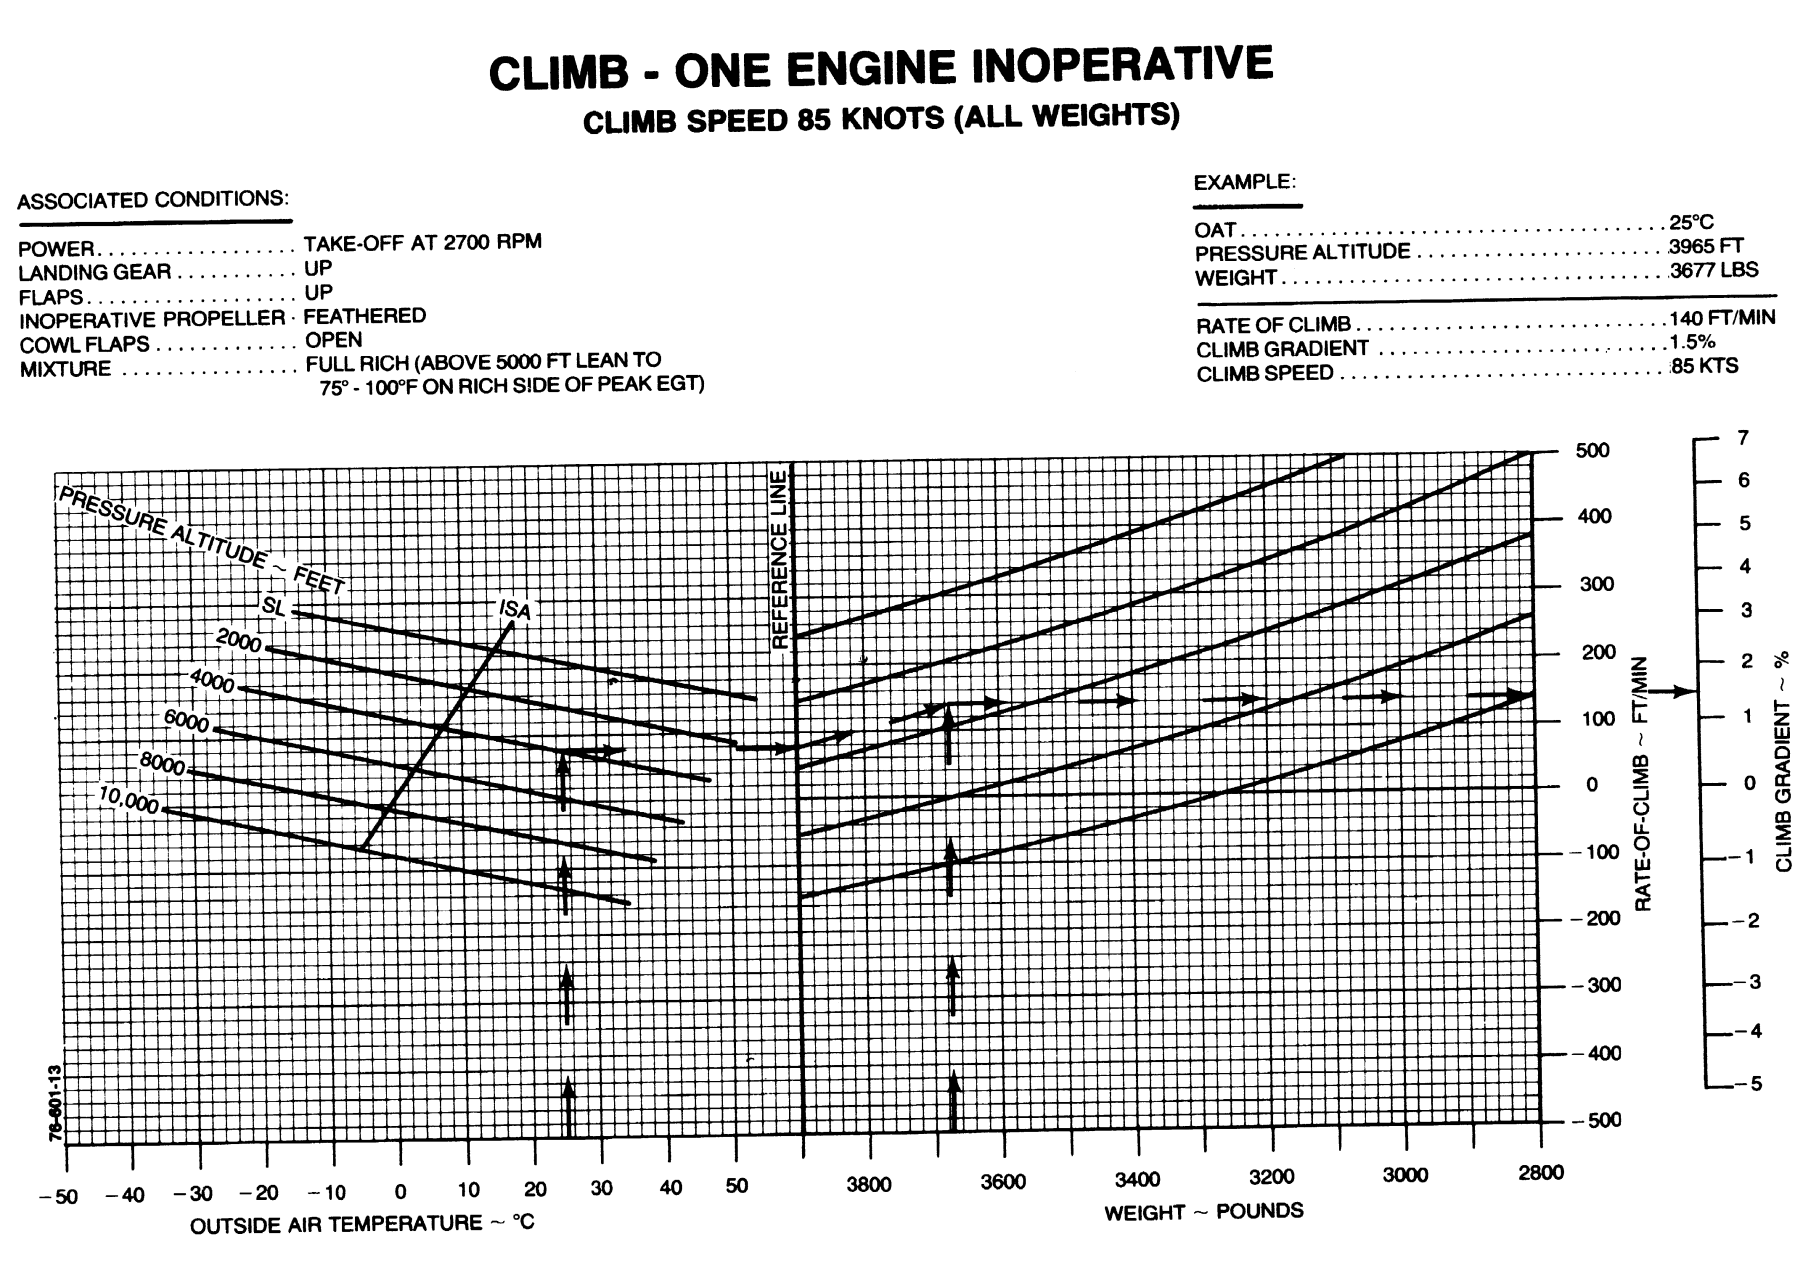
\includegraphics[width=0.9\linewidth]{duchess-1eo}
\end{center}
\end{figure}

\section{Time, Fuel, and Distance to Climb}

\begin{figure}[H]
\begin{center}
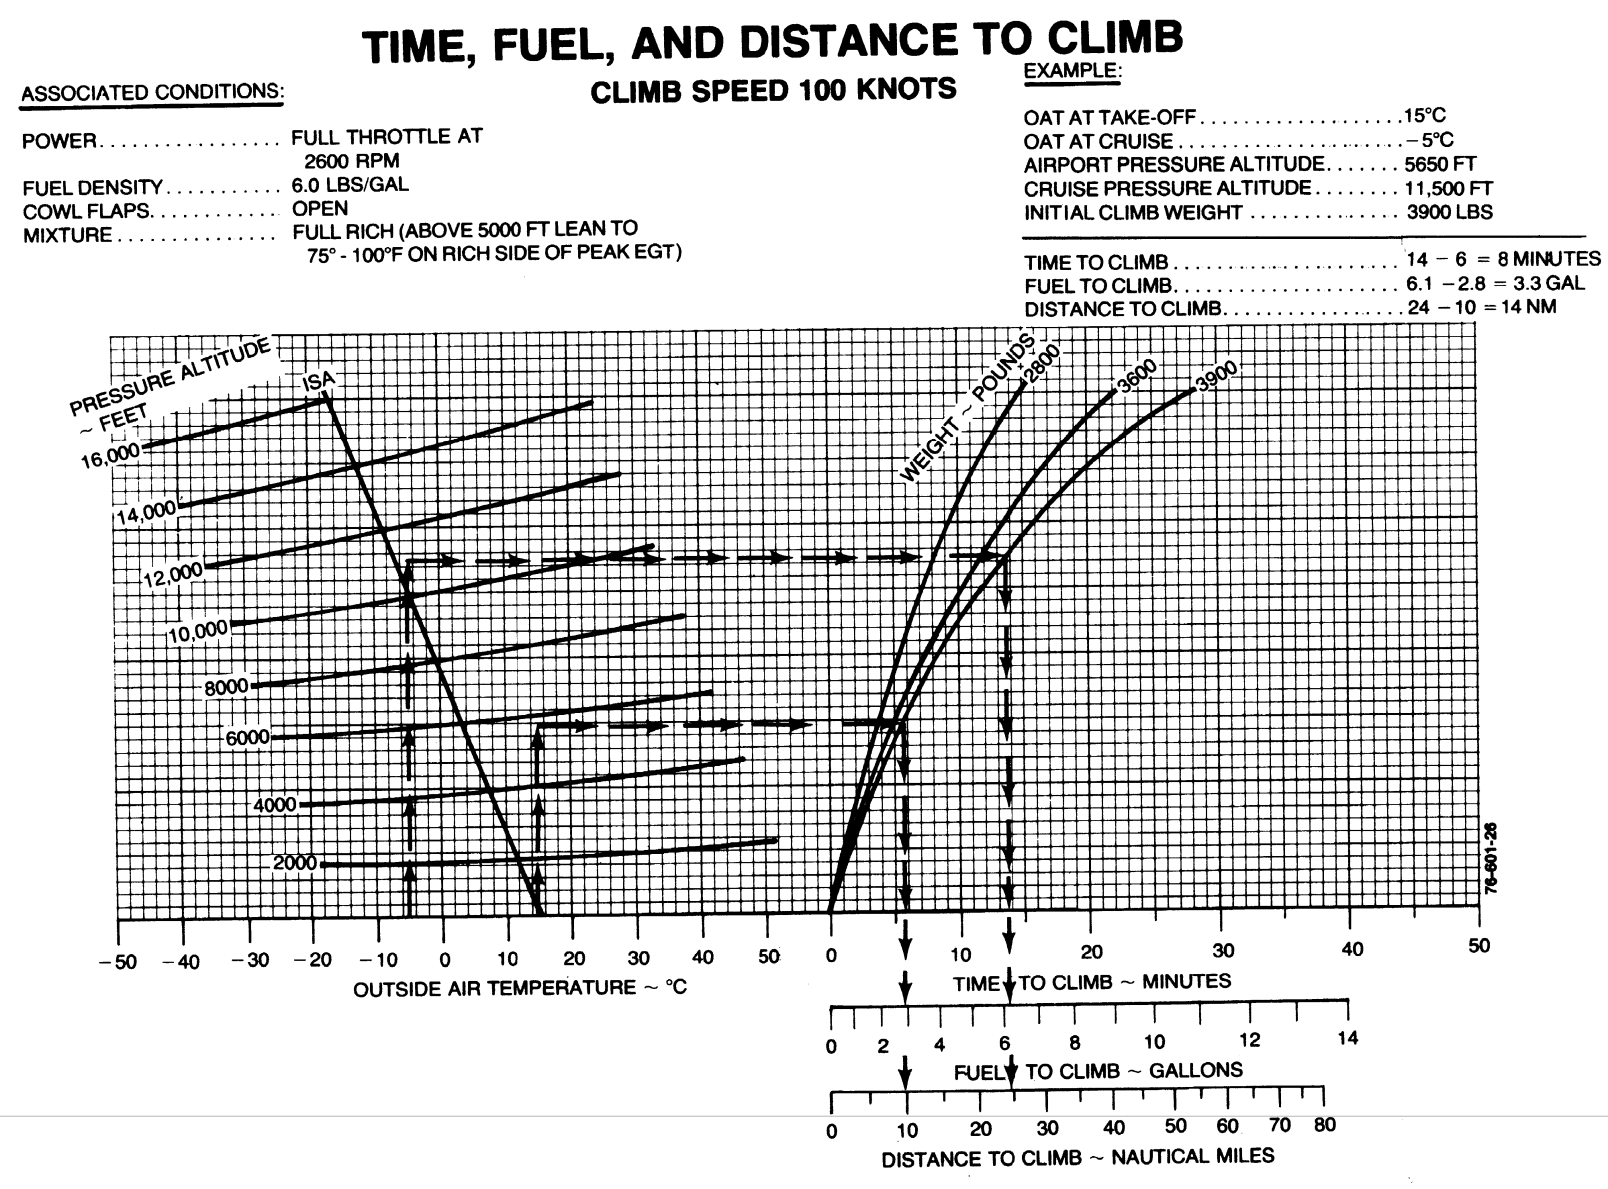
\includegraphics[width=1.0\linewidth]{duchess-tfd}
\end{center}
\end{figure}

\emph{Memory aid:}

\begin{table}[H]
\begin{tabular}{l|l|l|l}
      & \multicolumn{1}{c|}{\begin{tabular}[c]{@{}c@{}}min\\ T\end{tabular}} & \multicolumn{1}{c|}{\begin{tabular}[c]{@{}c@{}}gal\\ F\end{tabular}} & \multicolumn{1}{c}{\begin{tabular}[c]{@{}c@{}}nmi\\ D\end{tabular}} \\ \hline
4500  & 3.5                                                                  & 1.9                                                                  & 6                                                                   \\ \hline
GTU   & 0.2                                                                  & 0.1                                                                  & 1                                                                   \\ \hline
climb & 3                                                                    & 1.8                                                                  & 5                                                                  
\end{tabular}
\end{table}

\newpage

\section{Single-Engine Service Ceiling}

\begin{figure}[H]
\begin{center}
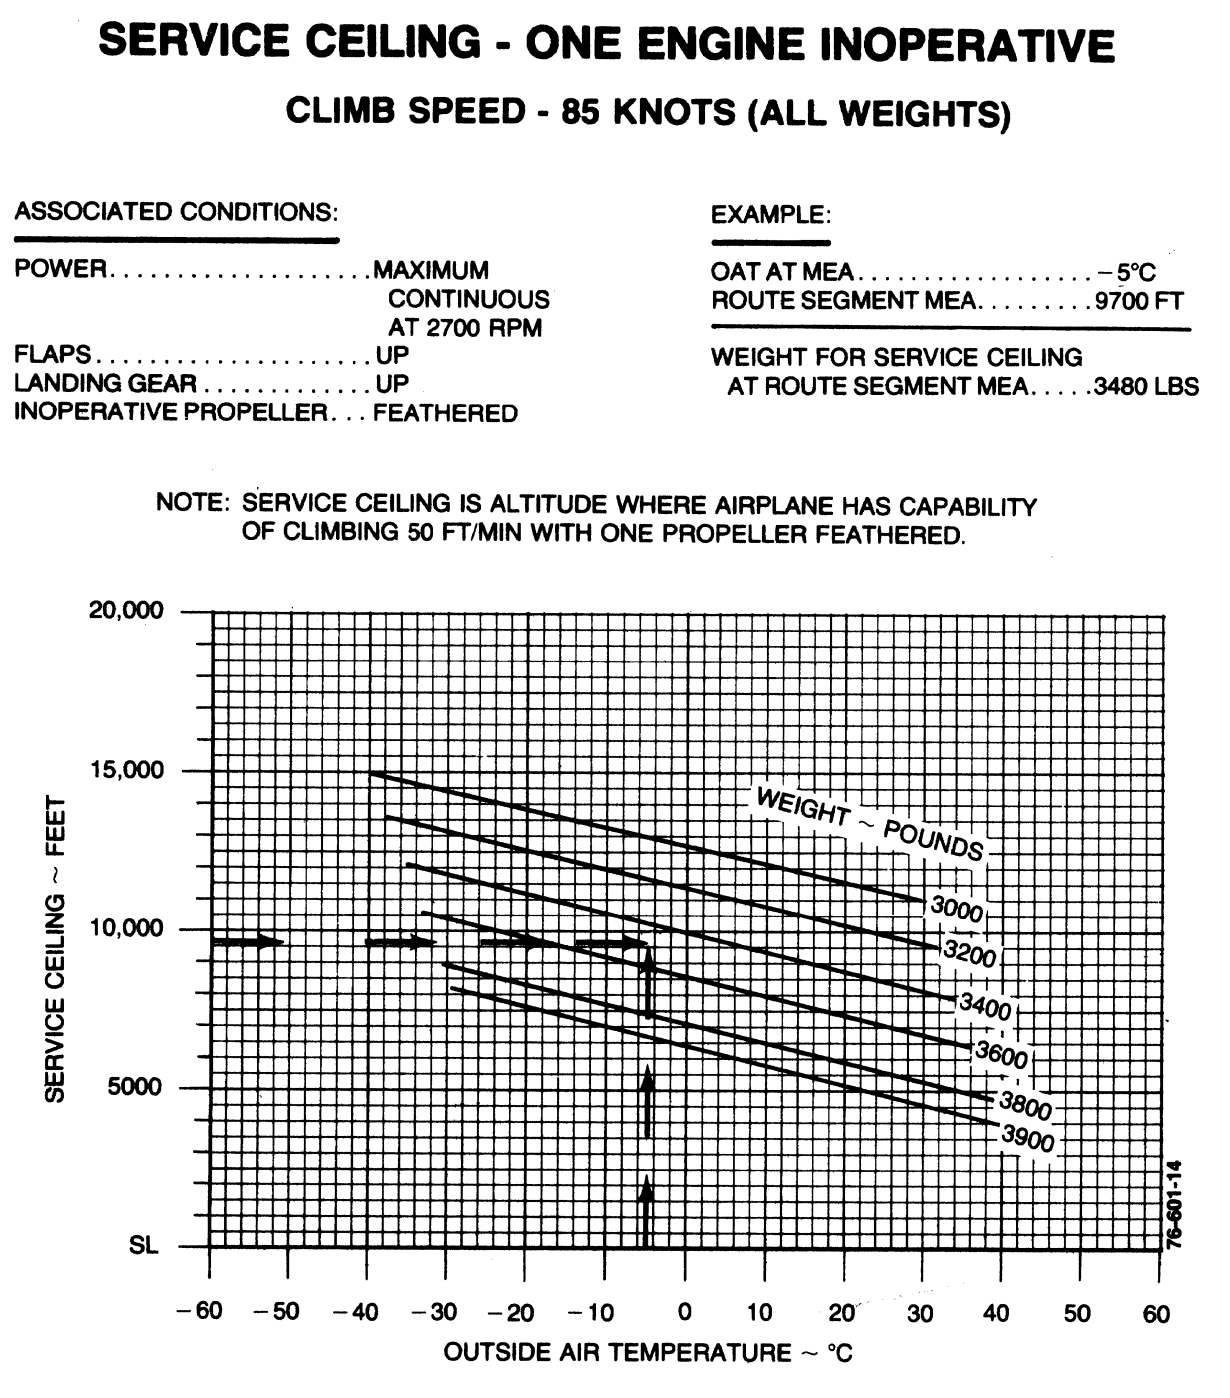
\includegraphics[width=1.0\linewidth]{duchess-secc}
\end{center}
\end{figure}

\newpage

\section{Cruise Performance, 24” Hg}

\begin{figure}[H]
\begin{center}
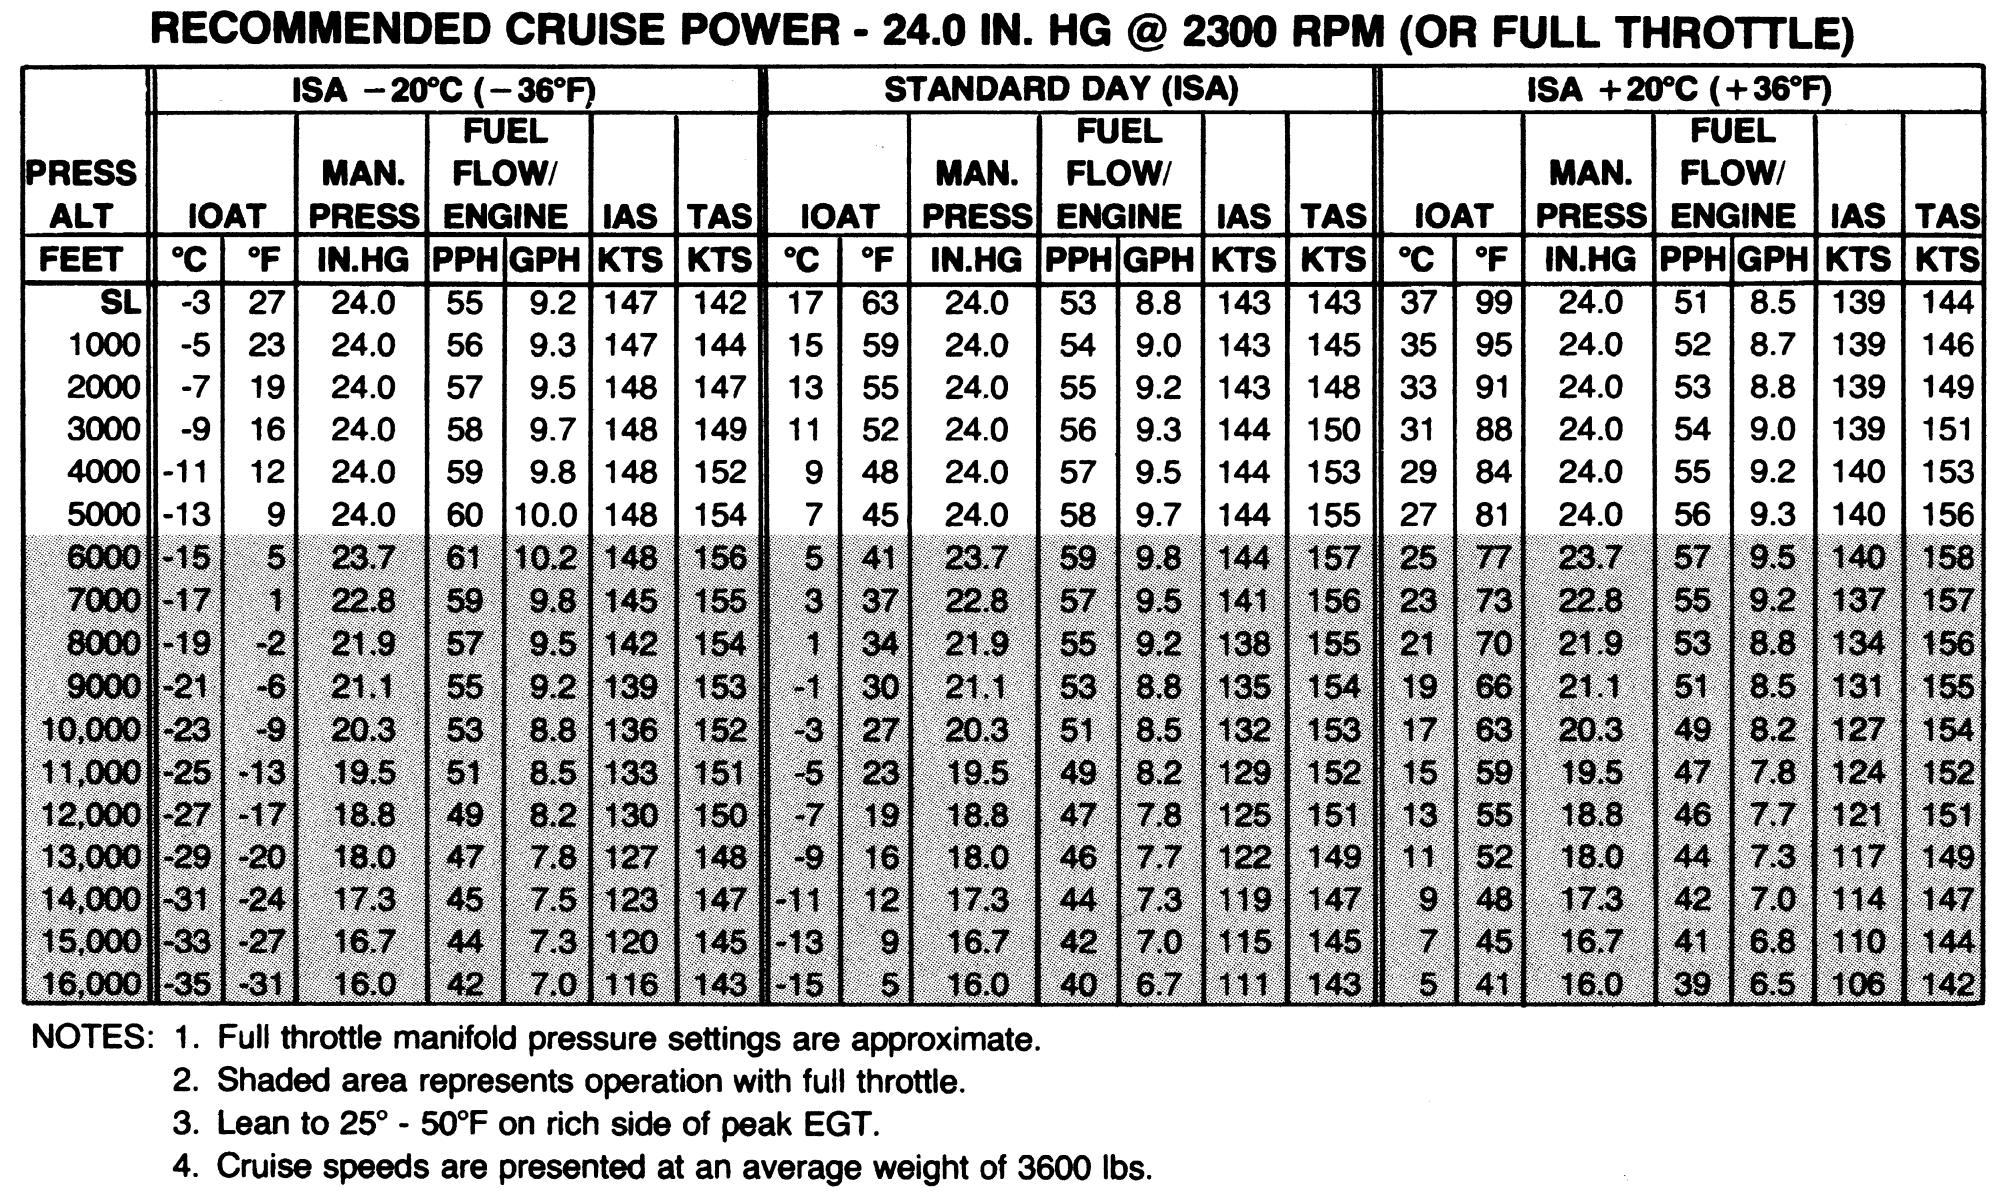
\includegraphics[width=0.9\linewidth]{duchess-24in}
\end{center}
\end{figure}

\section{Cruise Performance, 20” Hg}

\begin{figure}[H]
\begin{center}
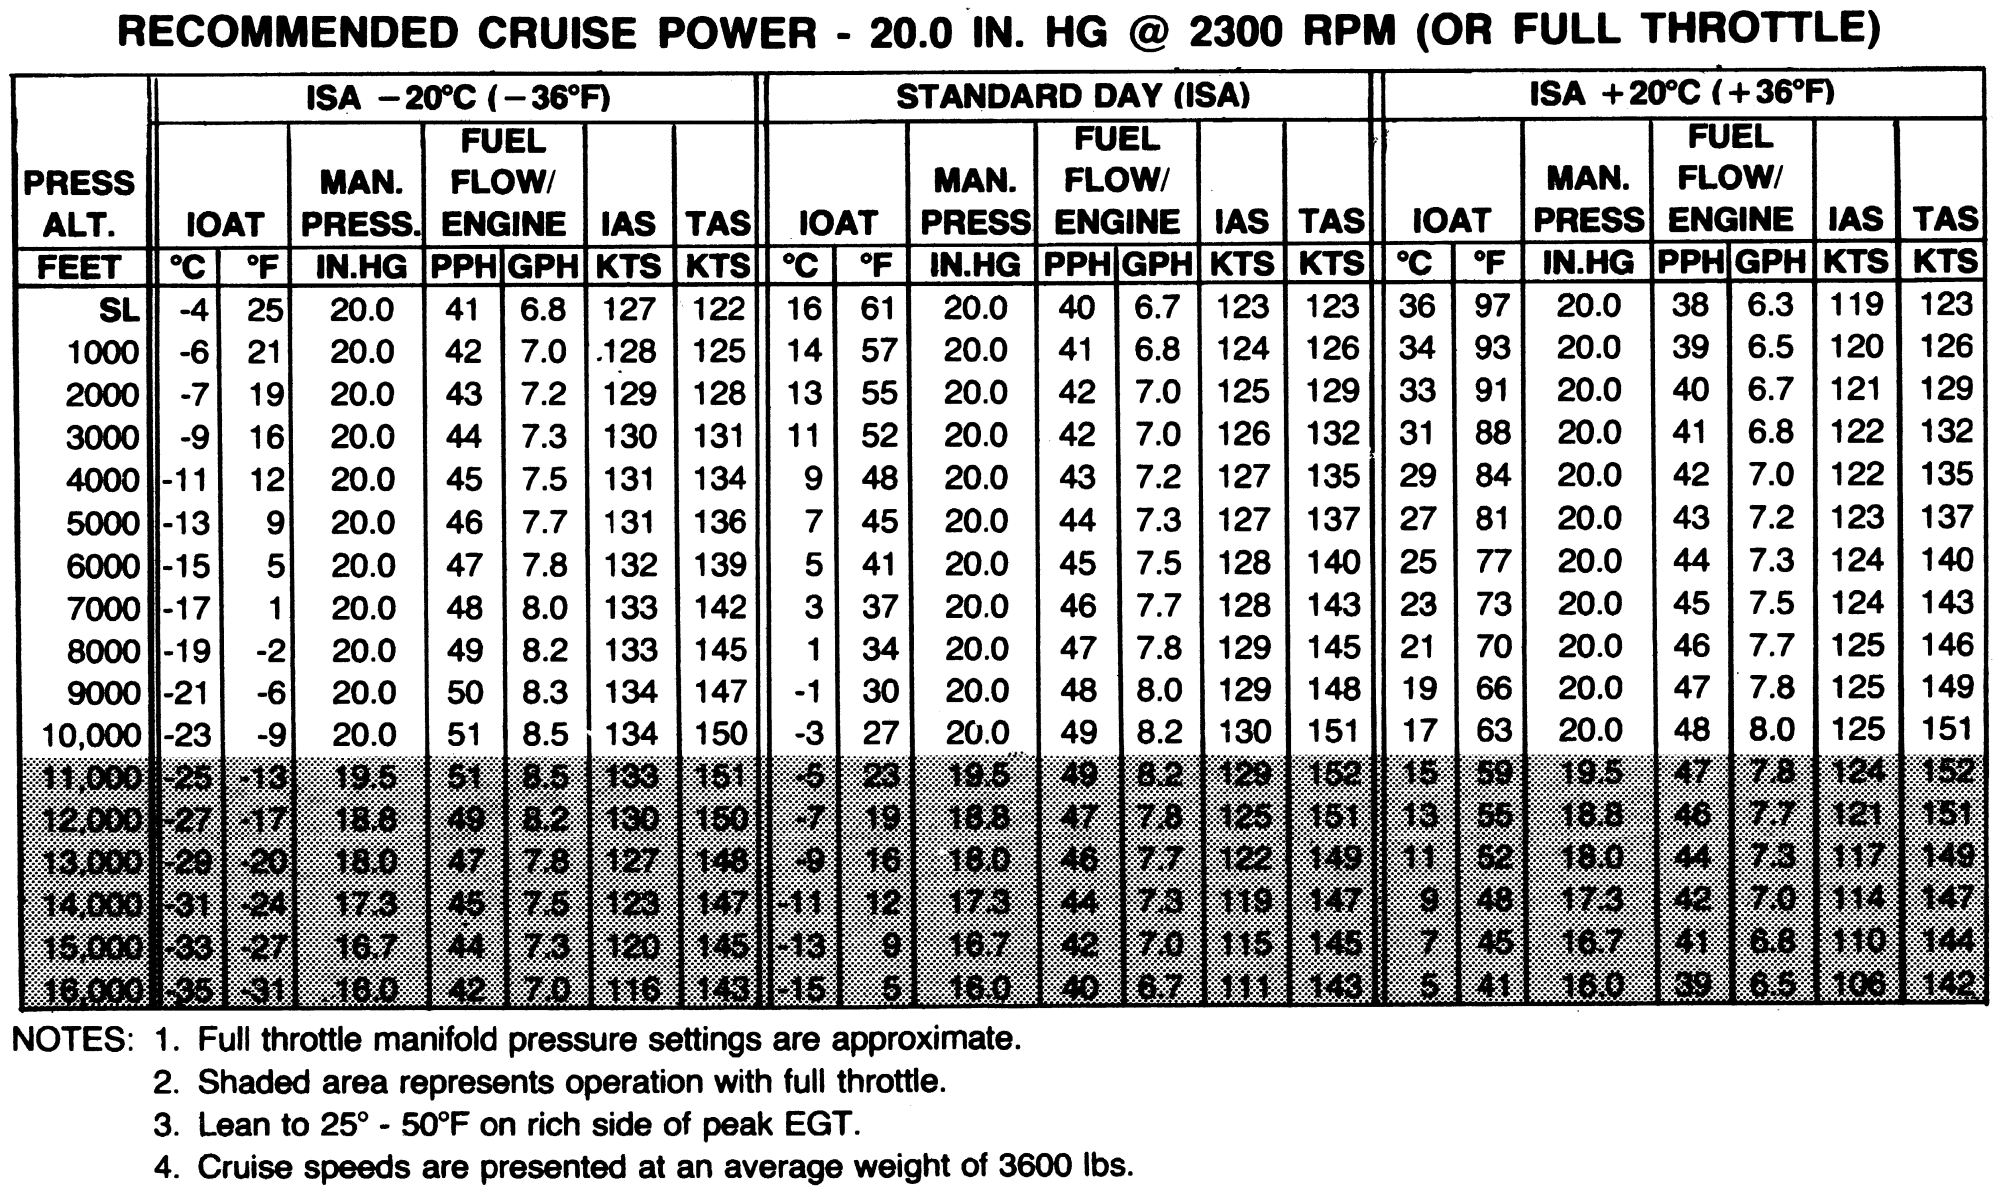
\includegraphics[width=0.9\linewidth]{duchess-20in}
\end{center}
\end{figure}

\newpage

\section{Landing Distance}

\begin{figure}[H]
\begin{center}
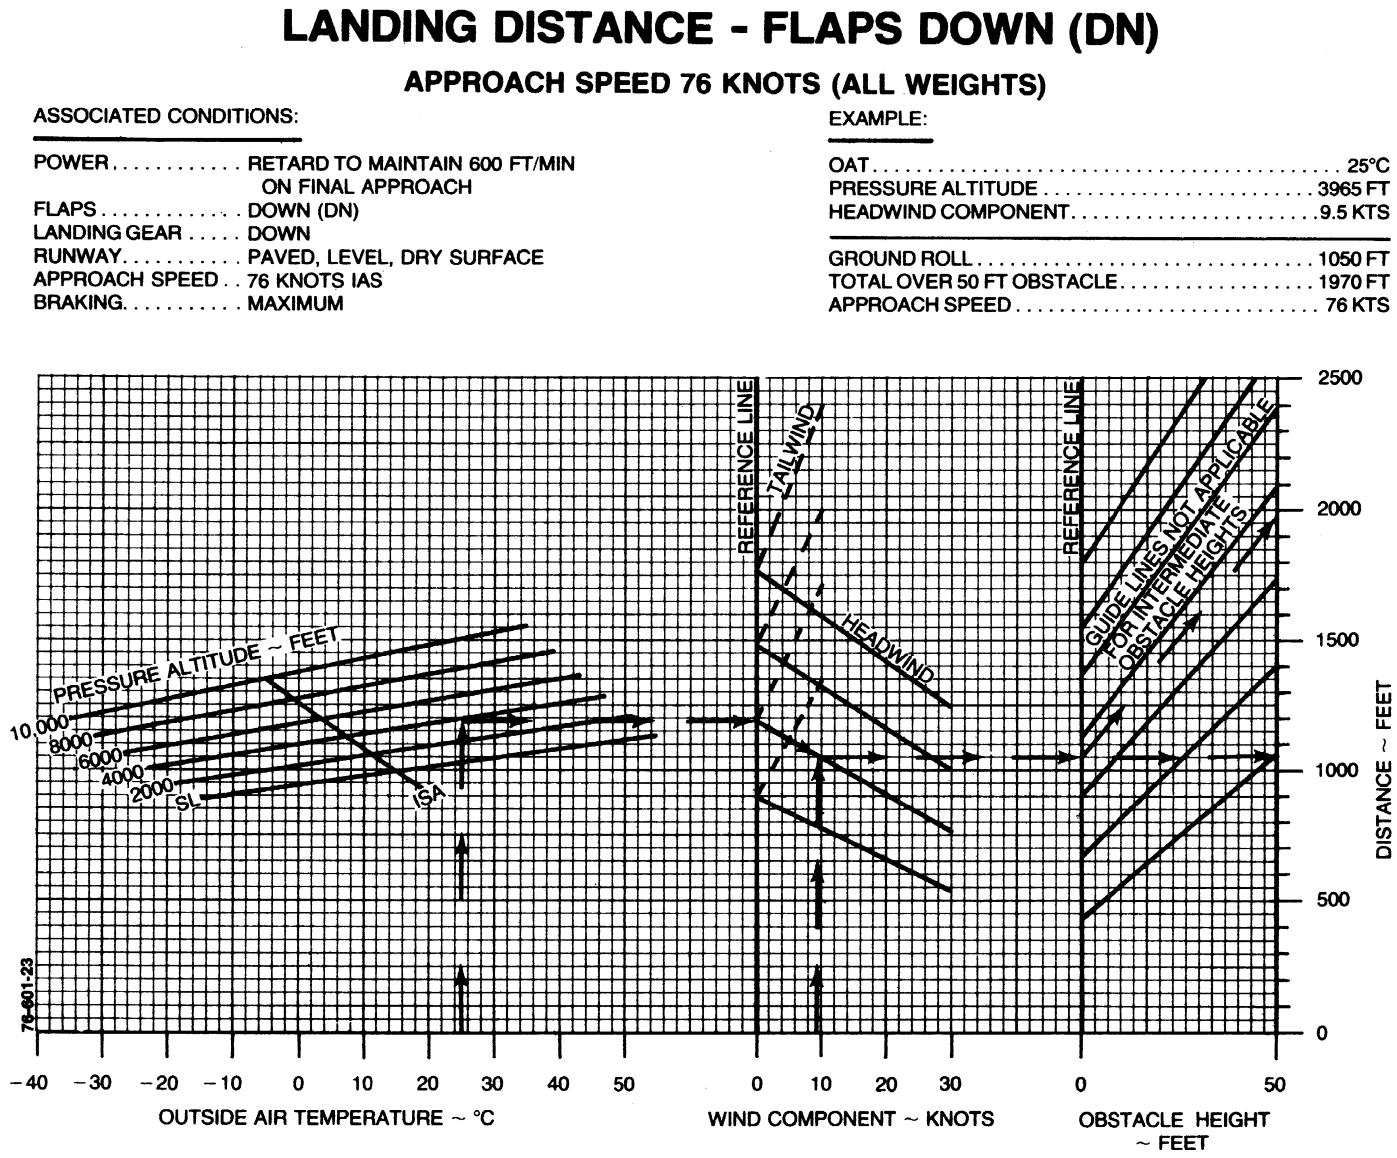
\includegraphics[width=1.0\linewidth]{duchess-ldg}
\end{center}
\end{figure}

\chapter{Weight and Balance}

Calculation of weight and balance in the Duchess is straightforward.
Note that the Duchess has a maximum zero
fuel weight, which restricts the useful load carried as passengers
and cargo. The maximum weight of the airplane
plus passengers and baggage must not exceed 3500 pounds – the rest
of the useful load must be carried as fuel.

See the figures available in the POH for information on loading arms and C.G. limits.

\begingroup
\renewcommand{\arraystretch}{1.1} % Default value: 1

\begin{table}[H]
\begin{tabular}%
  {>{\raggedright\arraybackslash}p{0.15\linewidth}%
   >{\centering\arraybackslash}p{0.2\linewidth}%
   >{\centering\arraybackslash}p{0.2\linewidth}%
   >{\centering\arraybackslash}p{0.2\linewidth}%
  }
                                                                                                        & \textbf{Weight}       & \textbf{x Arm}                                                                         & \textbf{= Moment}     \\ \cline{2-4} 
\multicolumn{1}{l|}{Basic Empty Condition}                                                              & \multicolumn{1}{c|}{} & \multicolumn{1}{c|}{}                                                                  & \multicolumn{1}{c|}{} \\ \cline{2-4} 
\multicolumn{1}{l|}{Pilot \& Front Passengers}                                                          & \multicolumn{1}{c|}{} & \multicolumn{1}{c|}{\begin{tabular}[c]{@{}c@{}}105 (forward)\\ 112 (aft)\end{tabular}} & \multicolumn{1}{c|}{} \\ \cline{2-4} 
\multicolumn{1}{l|}{Passengers – Row 2}                                                                 & \multicolumn{1}{c|}{} & \multicolumn{1}{c|}{144}                                                               & \multicolumn{1}{c|}{} \\ \cline{2-4} 
\multicolumn{1}{l|}{Baggage (200\# max)}                                                                & \multicolumn{1}{c|}{} & \multicolumn{1}{c|}{167}                                                               & \multicolumn{1}{c|}{} \\ \cline{2-4} 
\multicolumn{1}{l|}{\textbf{\begin{tabular}[c]{@{}l@{}}Zero Fuel Weight\\ (3500\# max)\end{tabular}}}   & \multicolumn{1}{c|}{} & \multicolumn{1}{c|}{}                                                                  & \multicolumn{1}{c|}{} \\ \cline{2-4} 
\multicolumn{1}{l|}{Fuel}                                                                               & \multicolumn{1}{c|}{} & \multicolumn{1}{c|}{117}                                                               & \multicolumn{1}{c|}{} \\ \cline{2-4} 
\multicolumn{1}{l|}{Ramp Condition}                                                                     & \multicolumn{1}{c|}{} & \multicolumn{1}{c|}{}                                                                  & \multicolumn{1}{c|}{} \\ \cline{2-4} 
\multicolumn{1}{l|}{Start/Taxi/Takeoff}                                                                 & \multicolumn{1}{c|}{} & \multicolumn{1}{c|}{}                                                                  & \multicolumn{1}{c|}{} \\ \cline{2-4} 
\multicolumn{1}{l|}{\textbf{\begin{tabular}[c]{@{}l@{}}Takeoff Condition\\ (3900\# max)\end{tabular}}}  & \multicolumn{1}{c|}{} & \multicolumn{1}{c|}{}                                                                  & \multicolumn{1}{c|}{} \\ \cline{2-4} 
\multicolumn{1}{l|}{Load Adjustments:}                                                                  & \multicolumn{1}{c|}{} & \multicolumn{1}{c|}{}                                                                  & \multicolumn{1}{c|}{} \\ \cline{2-4} 
\multicolumn{1}{l|}{Front seat}                                                                         & \multicolumn{1}{c|}{} & \multicolumn{1}{c|}{\begin{tabular}[c]{@{}c@{}}105 (forward)\\ 112 (aft)\end{tabular}} & \multicolumn{1}{c|}{} \\ \cline{2-4} 
\multicolumn{1}{l|}{Passenger}                                                                          & \multicolumn{1}{c|}{} & \multicolumn{1}{c|}{144}                                                               & \multicolumn{1}{c|}{} \\ \cline{2-4} 
\multicolumn{1}{l|}{Baggage}                                                                            & \multicolumn{1}{c|}{} & \multicolumn{1}{c|}{167}                                                               & \multicolumn{1}{c|}{} \\ \cline{2-4} 
\multicolumn{1}{l|}{Fuel}                                                                               & \multicolumn{1}{c|}{} & \multicolumn{1}{c|}{117}                                                               & \multicolumn{1}{c|}{} \\ \cline{2-4} 
\multicolumn{1}{l|}{\textbf{\begin{tabular}[c]{@{}l@{}}New Takeoff Weight\\ (3900\# max)\end{tabular}}} & \multicolumn{1}{c|}{} & \multicolumn{1}{c|}{}                                                                  & \multicolumn{1}{c|}{} \\ \cline{2-4} 
\multicolumn{1}{l|}{Fuel Burn}                                                                          & \multicolumn{1}{c|}{} & \multicolumn{1}{c|}{117}                                                               & \multicolumn{1}{c|}{} \\ \cline{2-4} 
\multicolumn{1}{l|}{\textbf{Landing Condition}}                                                         & \multicolumn{1}{c|}{} & \multicolumn{1}{c|}{}                                                                  & \multicolumn{1}{c|}{} \\ \cline{2-4} 
\end{tabular}
\end{table}
\endgroup


\chapter{Systems - Beechcraft Duchess BE-76}

\emph{Memory aid: N6001Y ME-119; N3733G ME-364}

\section{Engines}

The Duchess has two Lycoming 4 cylinder-engines – an O360 on the left, and an LO-360 (the ``L'' is for ``left'' turning) on the right. Both engines produce 180 horsepower at 2700 RPM and are air-cooled, direct drive,
horizontally opposed, reciprocating, normally aspirated engines. Oil capacity is 8 quarts maximum.

\section{Propellers}

\subsection{Propeller System Basics}

The Duchess has two 76-inch diameter, constant speed, full-feathering Hartzell propellers. The propellers are
counter-rotating: the left propeller turns clockwise and right propeller turns counterclockwise. Unlike most light
twins which have conventional propellers where both turn clockwise, there is no critical engine with counter-
rotating propellers. See the definition of critical engine in Section 1.

The propeller controls on the control console allow the pilot to select the governor's RPM range. Propeller governors
regulate oil pressure to control RPM by varying the blade angle (pitch) of the propeller to make it more efficient.
Oil pressure and aerodynamic twisting send the propeller out of feather to high RPM settings (low pitch=small blade
angle, taking small ``bites'' of air). Nitrogen pressure and a large spring, aided by counterweights, send the propeller
to low RPM (high pitch=high blade angle).

The oil pressure and nitrogen/spring pressure constantly oppose each other. When the propeller control is moved to
the feather position, the opposing oil pressure is released and the spring, air pressure and counterweights cause the
propeller to ``feather'' - a pitch of approximately 80\degree; this is a minimum drag condition. The propellers can be
unfeathered with the aid of unfeathering accumulators. When the propeller control is moved forward, stored oil
pressure is released which forces the propeller into a lower pitch. If this is done above 100 knots, the propeller
should windmill, allowing the engine to be re-started without the aid of the starter.

A feathering lock, operated by centrifugal force, prevents feathering during engine shut down by making it
impossible to feather any time the engine speed falls below 950 RPM. For this reason, when the pilot wishes to
feather a propeller, he must be sure to move the propeller control into the FEATHER position before the engine
speed drops below 950 RPM. This will not happen while airborne since the propeller will windmill faster than 950
RPM with normal propeller control settings. \emph{(see schematic)}

\subsection{Propeller Governor Operation}

The propeller governor is mounted on the accessory case on the rear of the engine. It contains a speeder spring,
which is directly controlled by the propeller lever in the cockpit, and flyweights which spin at engine RPM (see
propeller system diagram). When the pilot sets an RPM value with the propeller control, the engine attempts to
maintain that RPM setting by pitching the blades as required by the existing airspeed and power setting.

The propeller governor operates by regulating the flow of high-pressure oil into and out of the propeller hub.
Increasing oil pressure into the hub pitches the propeller blades flatter (higher RPM) and allowing oil to flow out of
the propeller hub allows the propeller to achieve a higher pitch (lower RPM or feather). The flow of oil is controlled
by a pilot valve in the governor which blocks the flow of oil to and from the propeller hub under normal conditions.

When the propeller RPM starts to increase (because of a momentary dive, for example) the flyweights are slung
away from the rotating shaft because of centrifugal force. This raises the shaft, which allows oil to flow from the
propeller hub to the oil sump, moving the blades to higher pitch and reestablishing the set RPM value. When the
propeller RPM starts to decrease, the counterweights have less centrifugal force slinging them away from the shaft,
and the speeder spring forces them inward. This moves the pilot valve in the opposite direction, which allows the
flow of high-pressure oil into the propeller hub, moving the blades to a flatter position and increasing RPM to the set
value.

At lower power settings and airspeeds, the propellers may be fully flat and RPM will decrease below the set value.
At this point, moving the propeller control fully forward will have no effect on engine RPM, since the blades are
already at their flattest pitch.

\emph{Memory aid: This is why the throttles change RPM when at idle.}

\section{Landing Gear}

The retractable tricycle landing gear uses shock absorbers on the main gear (approximately 2" extension) and an
oleo strut on the nose gear (approximately 4 1/4" extension) for shock absorption. The nose gear is steerable
through a spring-loaded linkage connected to the rudder pedals. A hydraulic dampener on the nose strut eliminates
shimmy. Toe brakes aid in steering the aircraft. The minimum wingtip turn radius is approximately 27' with the use
of differential power.

Retraction and extension of the gear is accomplished through the use of an electrically driven reversible hydraulic
pump and hydraulic system terminating in a hydraulic actuator assembly mounted in each wheel well. Retraction or
extension requires 6-8 seconds. The gear is held in the retracted position by 1250 to 1550 PSI of hydraulic pressure;
there are no locks to hold the gear in the retracted position. The landing gear may be hydraulically extended or
retracted, and may be lowered manually (below 100 knots) by turning a dump valve which releases pressure from
the retract side of the system allowing the gear to free fall to the down and locked position. If you lose hydraulic
pressure for some other reason, the gear will lower (free fall) to the down position and you will not be able to raise
it. If you lose electrical power the gear can be lowered manually but not raised. For any gear malfunction
ALWAYS refer to the checklist.

\emph{Memory aid: Gear is electrically driven, hydraulically actuated. Pressure holds it up. Lack of pressure causes gear to free fall. That lets us drop gear in an emergency.}

Three green lights, one for each landing gear, are illuminated whenever the landing gear are down and locked. The
red light illuminates any time the gear is in transit, indicating that the hydraulic pump is active. All of the lights will
be extinguished when the gear is up. Pressing the face of each indicator light will verify that the lights are
functional. The intensity of the lamps can be controlled by turning the lens holder on each lamp (counterclockwise
is brighter, full clockwise will appear that the bulb is out). In addition, the 4 gear indicator lights are
interchangeable with each other to verify that you do not have a burned out bulb.

In the retract mode the electric pump/motor forces hydraulic fluid to the retract side of the system. A pressure
switch shuts off the motor (and extinguishes the red in-transit light) when the system pressure reaches approximately
1550 PSI. If pressure drops to approximately 1250 PSI the motor will again be activated, and the red in-transit light
will illuminate. An uplock check valve in the pump retains this pressure to hold the gear up. In addition, landing
gear retraction operation is protected by a time-delay relay, which will disengage electrical power to the pump/motor
after 30 seconds of continuous operation. If the landing gear in-transit light remains illuminated, it indicates
improper response of the landing gear. The relay can be reset by moving the gear switch to the down position.

\emph{Memory aid: Watch for gear in transit light illuminating in flight, this could indicate a failing pump or a leak in the system.}

In the extend mode the electric motor forces hydraulic fluid to the extend side of the system. Main gear downlock is
accomplished by over-center travel of a spring-held side brace. Nose gear downlock is accomplished by over-center
travel of the drag link and a mechanically actuated downlock. After the gear are down and locked, system pressure
will bleed back to zero. Down limit switches, located on each gear, will allow the pump/motor to run until all three
gear are down and locked.

To prevent inadvertent retraction of the landing gear on the ground, a safety pressure switch is installed in the pitot
system to deactivate the hydraulic pump circuit when impact air pressure is below approximately 59 to 63 knots.

\emph{Memory aid: Do not retract the gear on the ground! What if the safety pressure switch is inoperative?}

If either or both throttles are retarded below an engine setting sufficient to sustain flight and the landing gear are not
fully extended, the landing gear warning horn will sound intermittently. An optional gear warning silence button
\emph{(not installed in either of the PCA Duchess aircraft as of this writing)}
allows the pilot to silence the alarm if one throttle is retarded. Additionally, when the flaps are extended beyond
about 16\degree, the warning horn will sound, regardless of throttle position, if the landing gear is not down and locked.
\emph{(see schematic)}

System Operation Notes:
\begin{enumerate}
\item The pilot moves the propeller control, which applies or relieves pressure from the speeder spring.
\item Flyweights and speeder spring move up and down, pushing or opening the pilot valve.
\item Oil from the engine driven governor oil boost pump is pushed toward the pilot value.
\item Oil moves past the pilot valve toward the propeller hub.
\item Oil fills the propeller hub in the direction of the low pitch stop.
\item The low pitch stop sets the high RPM limit.
\end{enumerate}

\section{Brakes and Tires}

Single-disk, double-piston Cleveland hydraulic brakes are fitted to the main gear. Each rudder pedal is fitted with a
master cylinder, which pressurizes the two pistons on either of the brake assemblies, forcing the linings to press
against the disk. To set the parking brake, pull the control out and pump both toe pedals until solid resistance is felt.
Push the control in to release the brakes. The hydraulic brake fluid reservoir is accessible through the nose
compartment. Fluid level is checked with the attached dipstick. The hydraulic system for the brakes is independent
of the gear. The main gear have 6.00-6 tires, and the nose gear has 5.00-5 tires. Normal inflation is 38 PSI for all
tires.

\section{Flaps and Trim}

Electrically actuated wing flaps are controlled by a three-position switch: UP, OFF, and DOWN. A dial type
indicator has position markings for UP, 10, 20, and DN (max is 35\degree{}). Limit switches interrupt power to the motor
when the flaps reach the extremes of travel. Intermediate flap positions can be obtained by placing the switch in the
off position during extension or retraction. Additionally, there is a micro switch activated at the 16\degree{} position which
is connected to the gear and stall warning circuits.

The elevator and rudder have cable-operated flight-adjustable trim tabs. The aileron control system has a trimmer
which functions by applying tension on the aileron control cables. Each control incorporates a mechanical position
indicator. The elevator trim may be operated manually or electrically.

\emph{Memory aid: $V_{FE}$ 120 KIAS @ 10 \degree{} - 20 \degree{}, 110 KIAS @ 35 \degree.}

\section{Pressure (Pneumatic) System}

Pressure for the attitude indicator and directional gyro is supplied by two engine-driven dry pressure pumps,
interconnected to form a single system. This is different from many light planes, which use vacuum to draw air
through the gyro instruments. If either pump fails, check valves automatically close and the remaining pump
continues to pressurize the system. Two red buttons on the pressure gauge indicate if that pump has failed. The HSI
is operated by the electrical system and therefore is not affected by a failure in the vacuum system.
\emph{(see schematic)}

\section{Pitot-Static System}

The Pitot tube is located outboard on the left wing. Pitot heat is available. The pitot system incorporates a pressure
switch, which prevents inadvertent gear retraction under approximately 60 knots. Static air is taken from flush static
ports located on each side of the fuselage. The alternate static air source is selectable on the lower left sidewall.
This lever also functions as the static system drain.

\section{Stall Warning System}

A stall warning sensing vane is installed on the leading edge of each wing. With flap settings of 0-15\degree{} the vane on
the left wing activates the warning horn. With flap settings of 16\degree{} or more the vane on the right wing activates the
system.

\section{Fuel System}

The airplane is designed for operation on grade 100 (green) or 100LL (blue) aviation gasoline. Two wing tanks hold
103 total gallons (100 usable). The filler neck of each tank contains a visual measuring tab to facilitate partial
filling. The sump drain on each tank can be locked open to offload fuel. There are eight fuel drain points. Each
engine has an engine driven fuel pump and an electrically driven boost pump, which serves as a backup and is used
for engine starts, takeoff, and landing. There are 3 positions on each fuel selector (on, off, and crossfeed). In
crossfeed, the engine will draw fuel from the opposite side in order to maintain a fuel balance during single engine
operations. Crossfeed should be used in level flight only. Each magneto/start switch incorporates a PUSH TO
PRIME function to aid in engine starting. A minimum of 9 gallons is required in each wing prior to takeoff.
\emph{(see schematic)}

\section{Heater and Defrost System}

A 45,000 BTU-per-hour combustion air heater, located on the right side in the nose compartment, provides heated
air for cabin warming and windshield defrosting. The heater system consists of a combustion air heater, a three-
position control switch, three push-pull control knobs, a heater circuit breaker, a manual reset limit (overheat) switch
(inaccessible in flight), a combustion air blower, a ventilation air blower, and a duct thermostat. The system uses
two thirds of a gallon per hour of fuel from the right wing. To operate, the cabin air outlet must be at least halfway
open.

\emph{Memory aid: The heater is deactivated in PCA aircraft. The external heater intake vents are covered for cold weather operations.}

\section{Electrical System}

\emph{Memory aid: N6001Y ME-119; N3733G ME-364}

One 24-volt, 15.5 ampere-hour, lead-acid battery is installed in the vented battery compartment just aft of the rear
bulkhead. Two self-exciting 55 ampere (for ME-183 and after, 28-volt: \textbf{N3733G}), or 60 ampere (for ME-1 thru ME-182, 14-
volt: \textbf{N6001Y}) belt driven alternators are installed, one on each engine. The systems are completely separate except for a bus
tie fuse, the mutual tie to the battery bus through two bus isolation circuit breakers, and the paralleling circuit
between the two voltage regulators (which makes sure the electrical load is equally shared between the two
alternators and keeps the voltage at 28 or 14 volts, depending upon the system installed). There are two load meters,
two pairs of alternator-out warning lights for over- or under-voltage conditions, and two over voltage relays which
will take the alternator off-line if the system exceeds operating voltage. The self-excitation feature will not come on
until approximately 1400 RPM, with a load capability of approximately 50\%, and a maximum load capability of
approximately 80\% should be obtainable at approximately 2300 RPM. Because they are self-exciting, the
alternators can function without a battery - but takeoff in this condition is prohibited.
\emph{(see schematic)}

\emph{Memory aid: L: All lights, turn coordinator, horns. R: Flaps, gear.}

\newpage

\section{System Schematics}

\subsection{Propeller System}

\begin{figure}[H]
\begin{center}
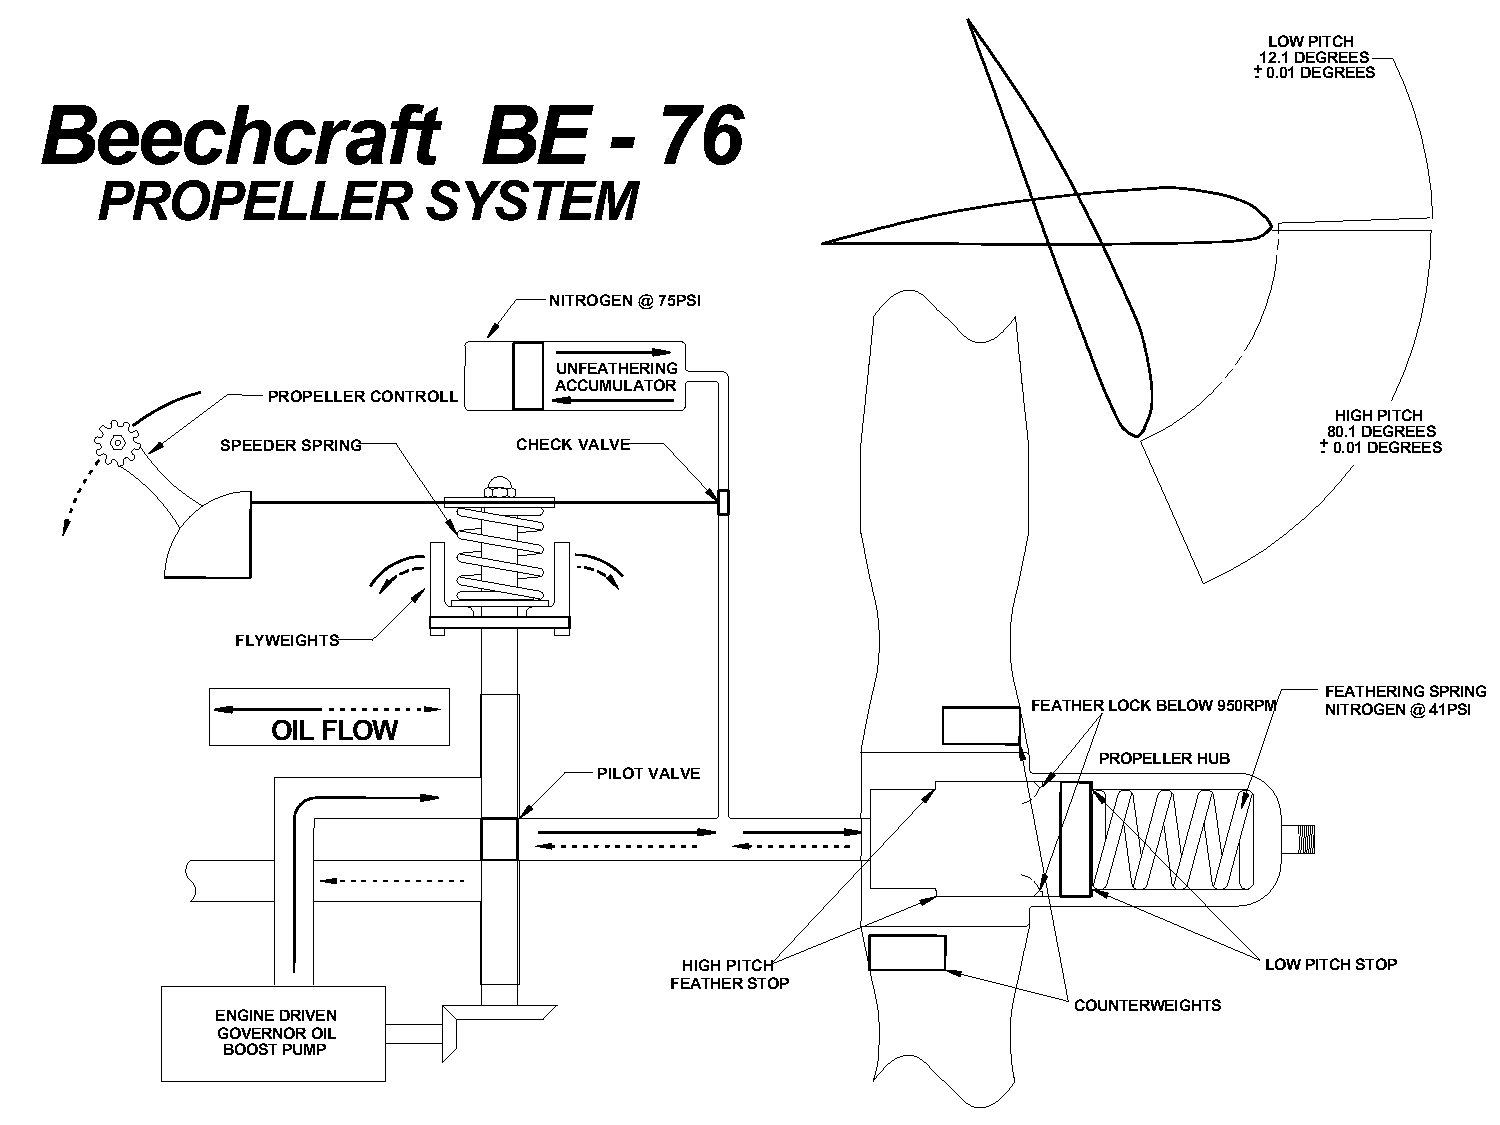
\includegraphics[width=1.0\linewidth]{be76-propeller}
\end{center}
\end{figure}

\newpage

\subsection{Landing Gear}

\begin{figure}[H]
\begin{center}
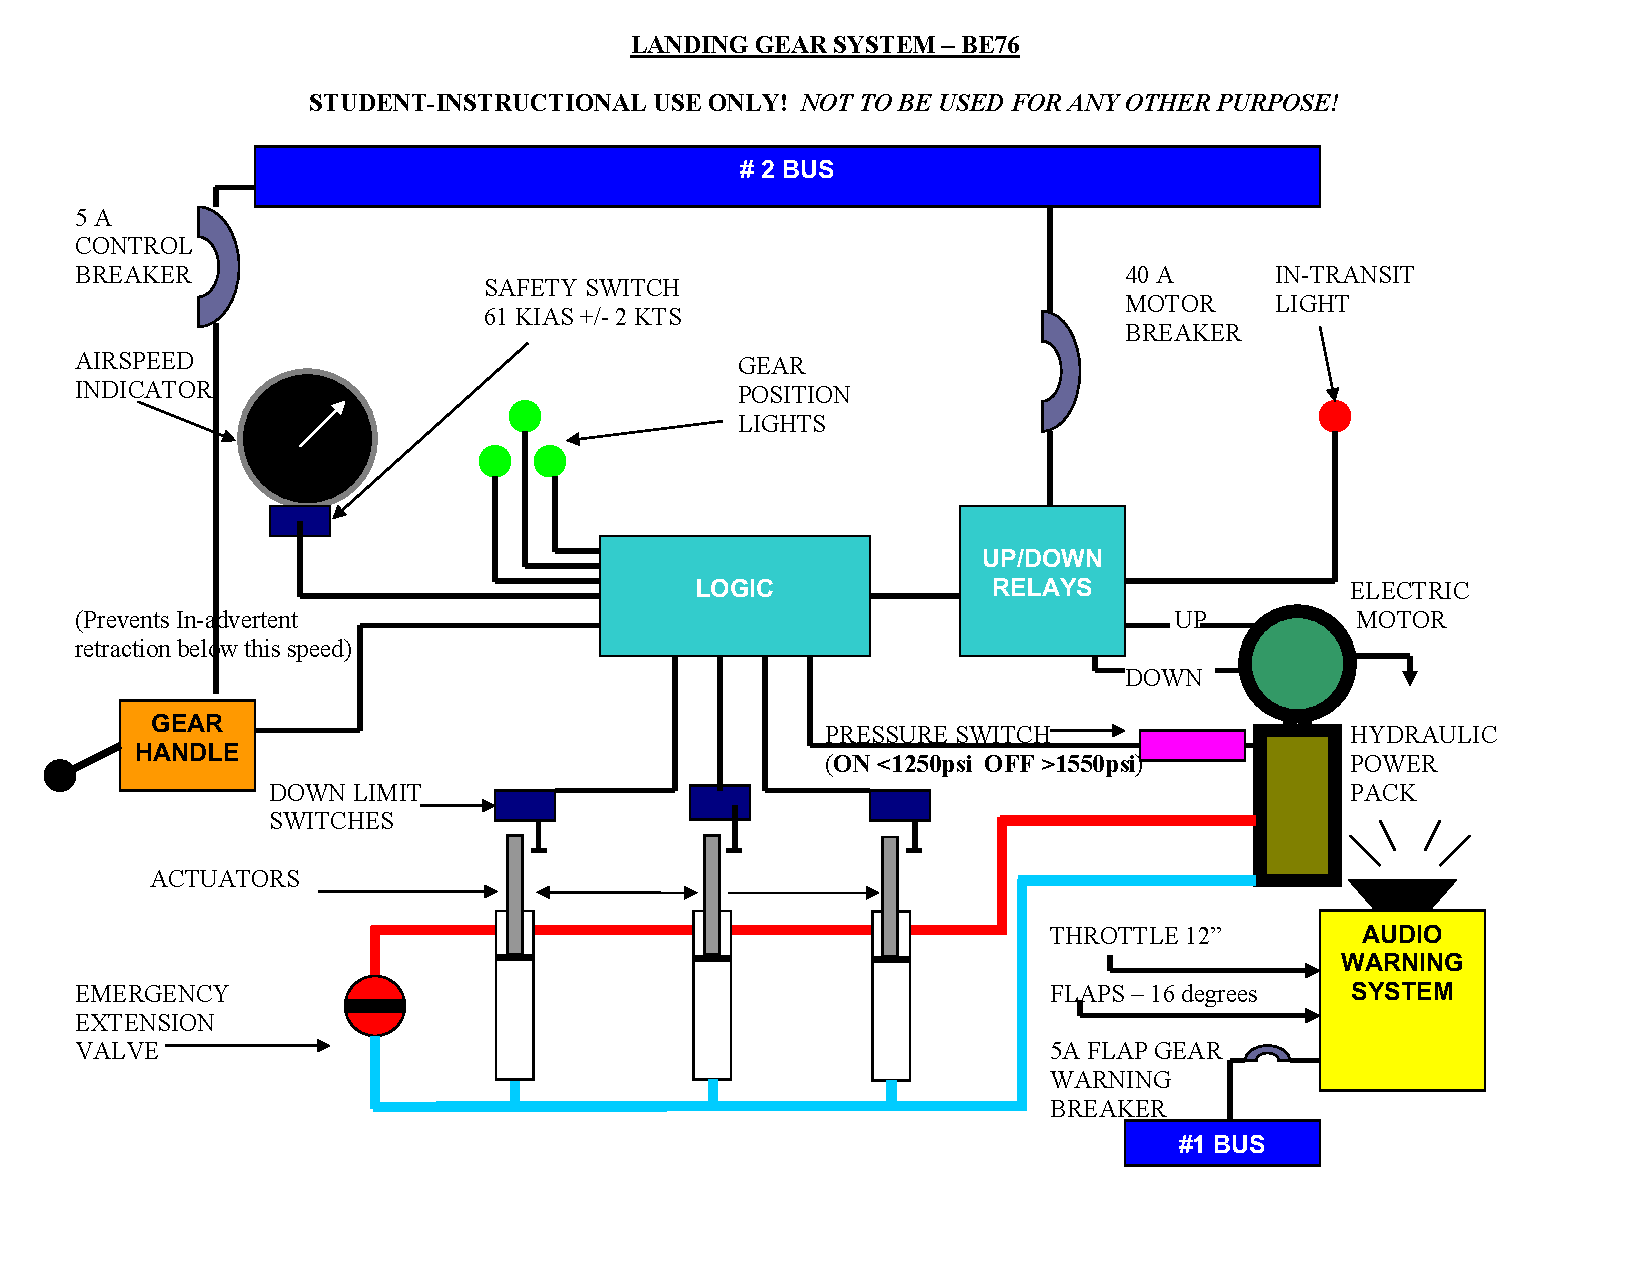
\includegraphics[width=1.0\linewidth]{be76-landinggear}
\end{center}
\end{figure}

\newpage

\subsection{Pressure System}

\begin{figure}[H]
\begin{center}
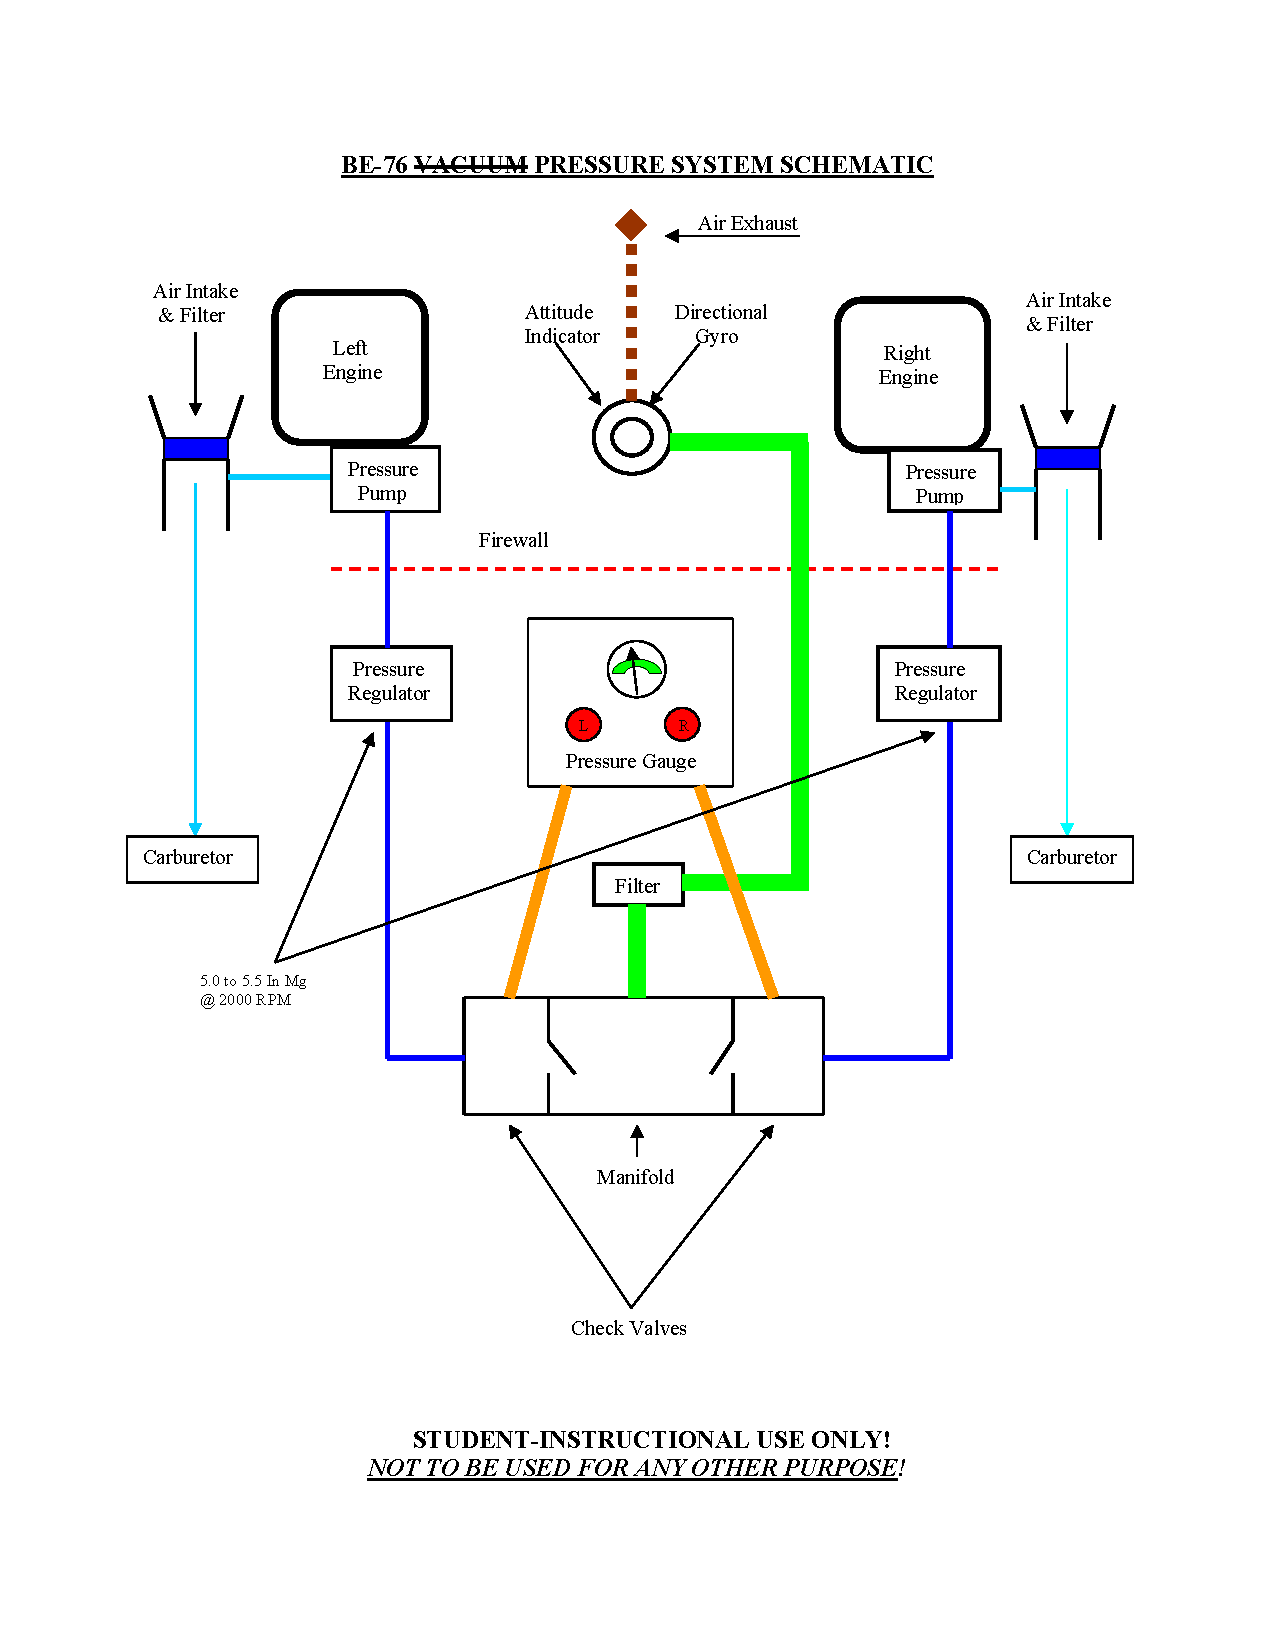
\includegraphics[width=1.0\linewidth]{be76-pressure}
\end{center}
\end{figure}

\newpage

\subsection{Fuel System}

\begin{figure}[H]
\begin{center}
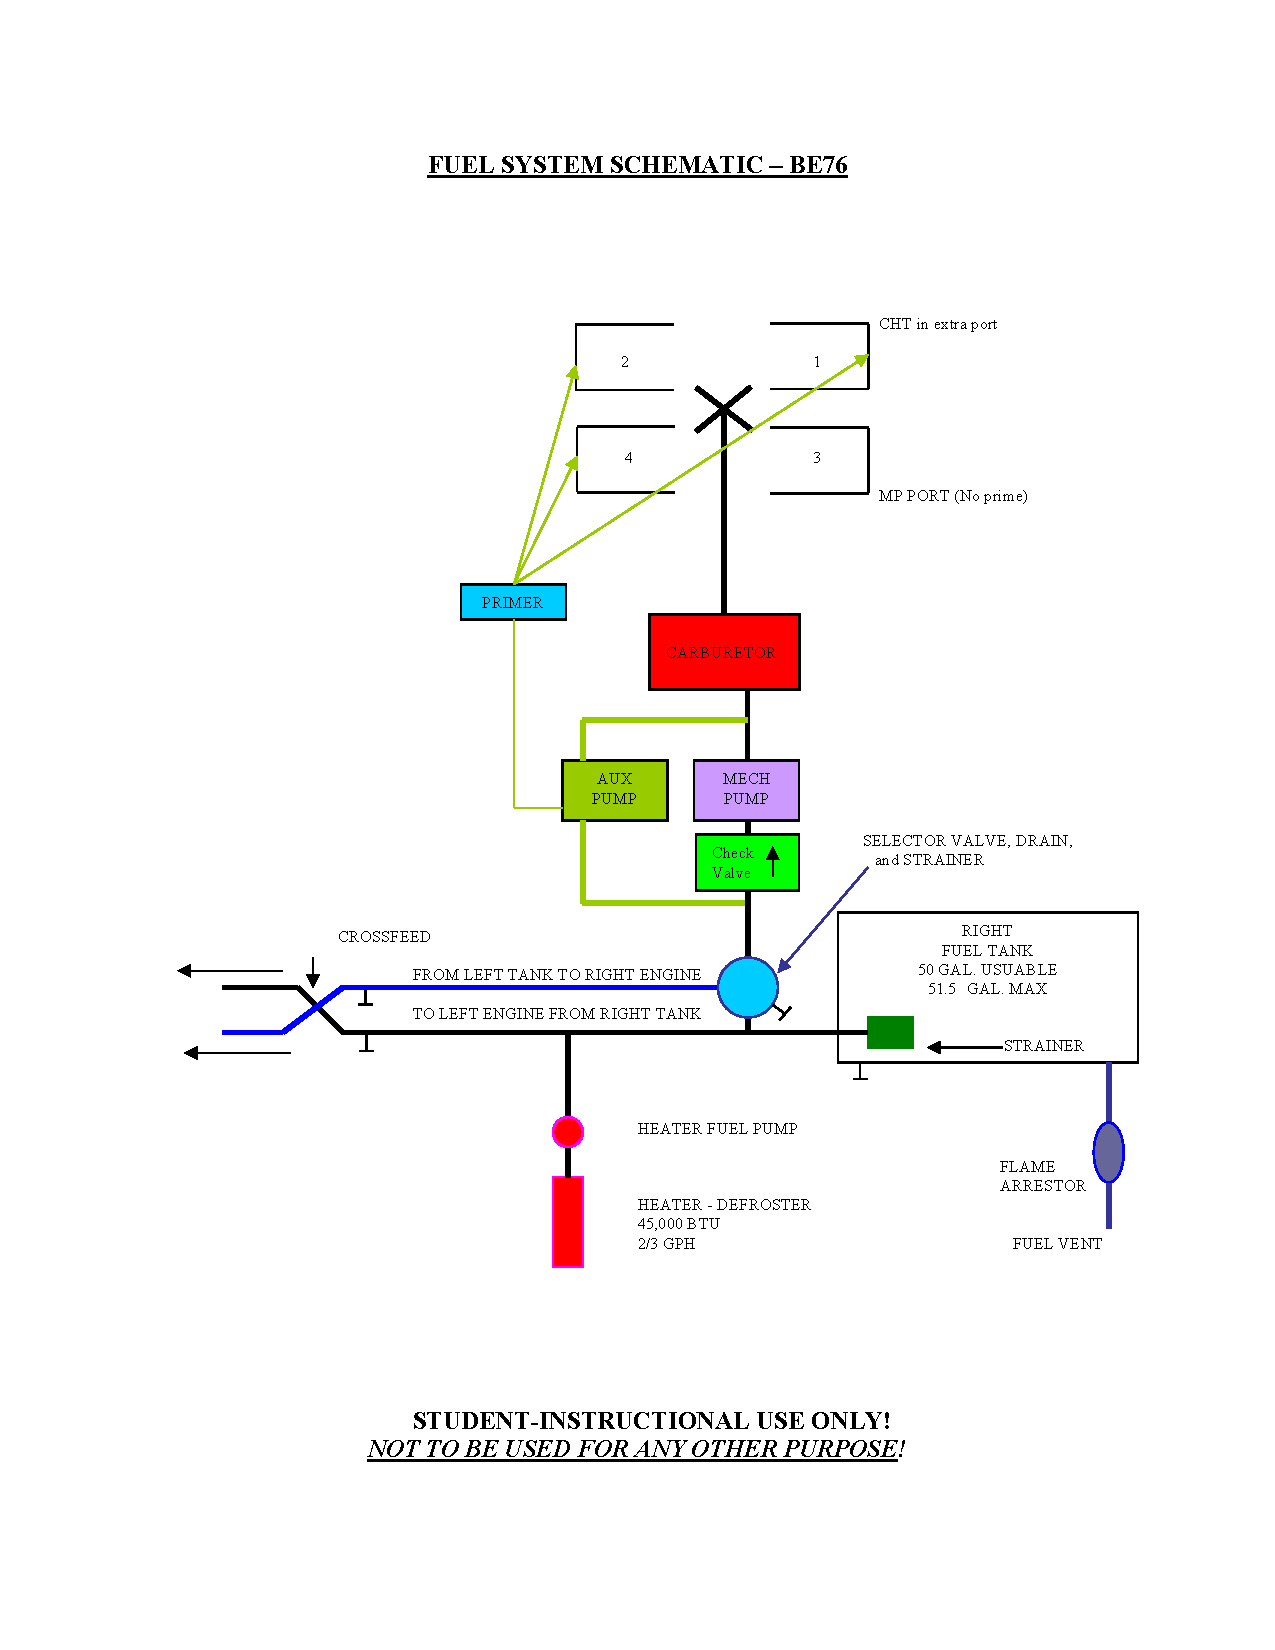
\includegraphics[width=1.0\linewidth]{be76-fuel}
\end{center}
\end{figure}

\newpage

\subsection{Electrical System}

\begin{figure}[H]
\begin{center}
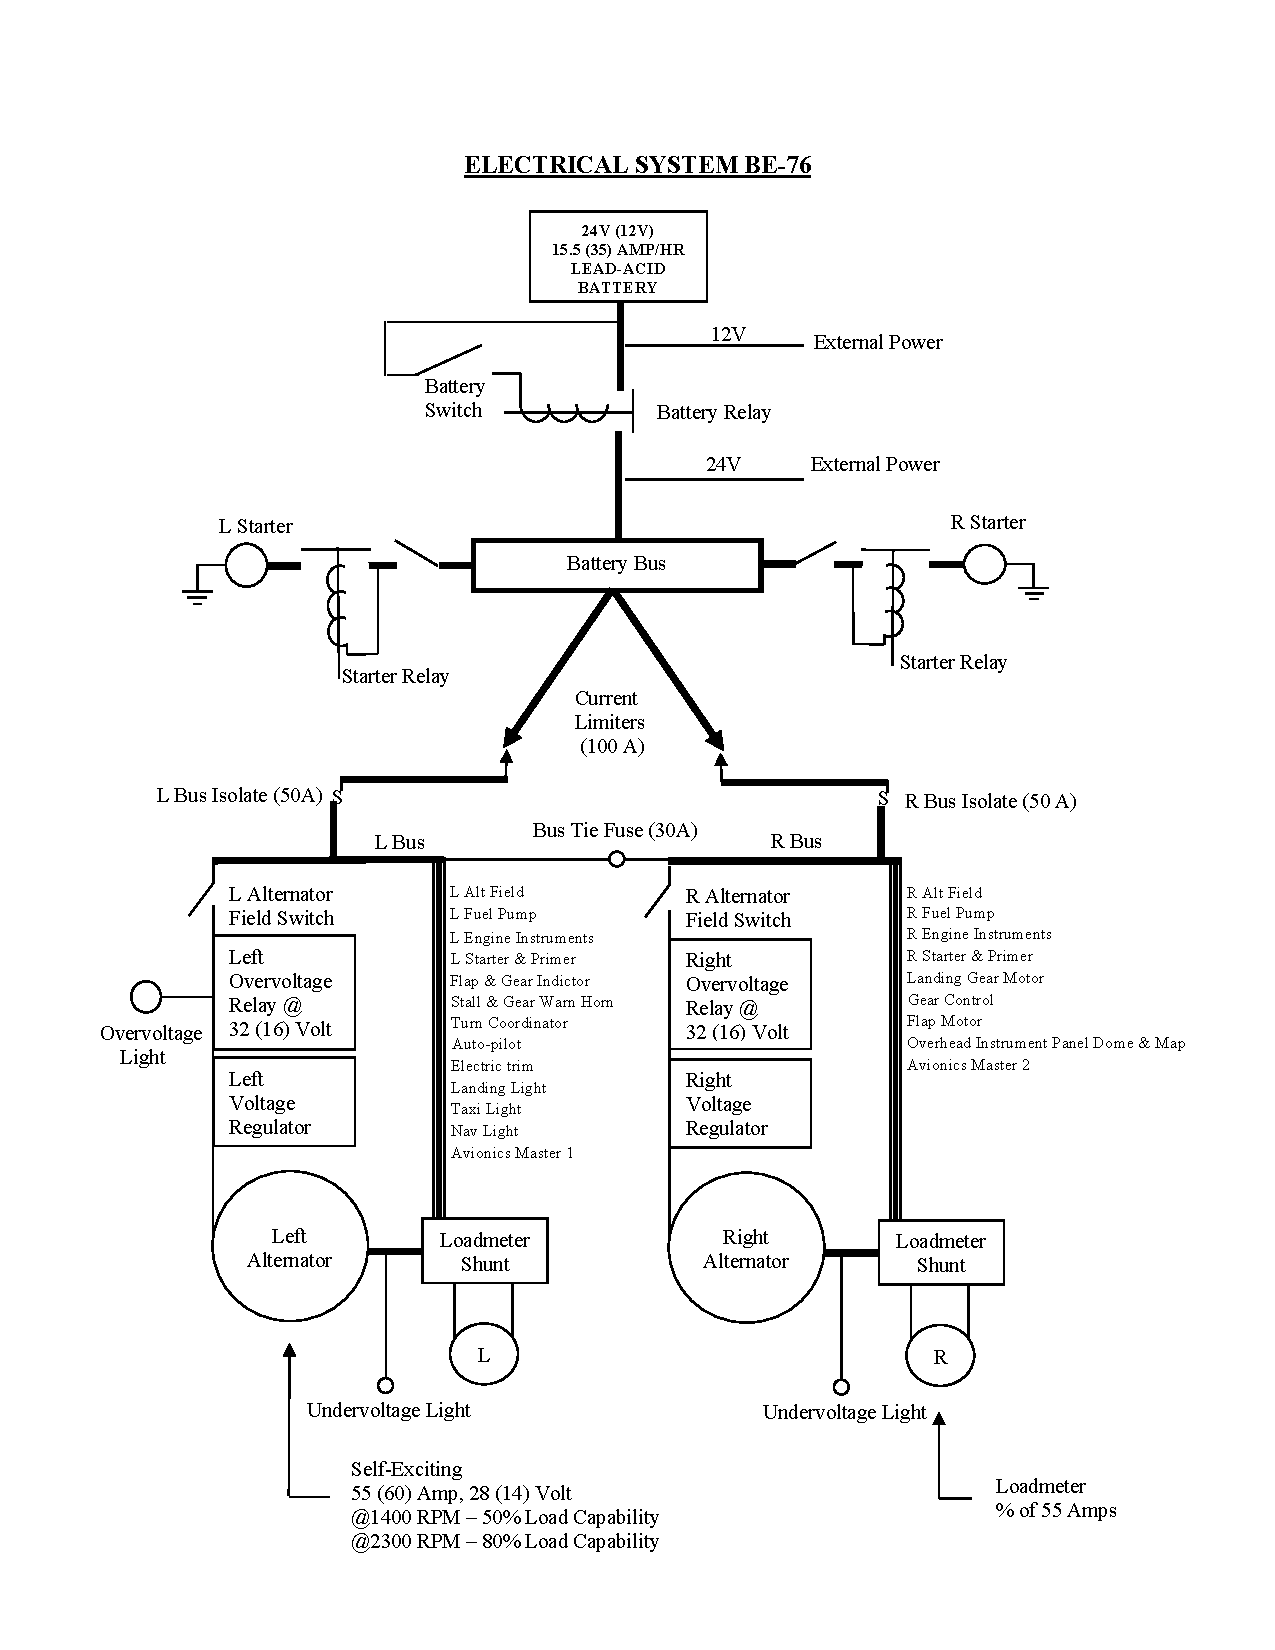
\includegraphics[width=1.0\linewidth]{be76-electrical}
\end{center}
\end{figure}

\chapter{Maneuvers}

\section{Introduction to Maneuvers}

All maneuvers begin and end the same way. Begin by clearing the area, followed by a power change (if required),
and a GUMP-CS check. The maneuvers end by re-establishing slow cruise (20''/2400), and doing a final GUMP-CS
check for cruise configuration.

\begin{table}[H]
\centering
\begin{tabular}{|c|l|c|c|}
\hline
                    &                                                 & \textbf{Maneuver Entry} & \textbf{Resume Cruise} \\ \hline
                    & \textcolor{blue}{\textbf{Power}}                & As Required             & 20'' MP                \\ \hline
\textcolor{blue}{G} & \textcolor{blue}{\textbf{G}}as (fuel selectors) & On                      & On                     \\
                    & \textcolor{blue}{\textbf{G}}as (boost pumps)    & On                      & Off                    \\ \hline
\textcolor{blue}{U} & \textcolor{blue}{\textbf{U}}ndercarriage        & As Required             & Up                     \\ \hline
\textcolor{blue}{M} & \textcolor{blue}{\textbf{M}}ixtures             & Rich                    & Cruise Lean            \\ \hline
\textcolor{blue}{P} & \textcolor{blue}{\textbf{Propellers}}           & As Required             & 2400 RPM               \\ \hline
\textcolor{blue}{C} & \textcolor{blue}{\textbf{C}}owl Flaps           & As Required             & Closed                 \\ \hline
\textcolor{blue}{S} & \textcolor{blue}{\textbf{S}}eat Belts           & Secure                  & Secure                 \\ \hline
\end{tabular}
\end{table}

Airman Certification Standards tables in this chapter are taken from from FAA-S-ACS-7B, Commercial Pilot for Airplane Category Airman Certification Standards, November 2023, and  FAA-S-ACS-25, Flight Instructor for Airplane Category, Airman Certification Standards, November 2023 as appropriate. Private pilot multi engine checkrides are rare, and maneuvers performed to the commercial standard are more than satisfactory for the private checkride's more forgiving tolerances.

\newpage

\section{Slow Flight}
\subsection{Maneuver Checklist}

\textbf{Perform clearing turns prior to maneuver. At least 3000' AGL.}

Set up maneuver:

\begin{table}[H]
\centering
\begin{tabular}{|c|l|c|c|}
\hline
                    &                                                 & \textbf{Maneuver Entry} & \textbf{Resume Cruise} \\ \hline
                    & \textcolor{blue}{\textbf{Power}}                & \textbf{15'' MP}        & 20'' MP                \\ \hline
\textcolor{blue}{G} & \textcolor{blue}{\textbf{G}}as (fuel selectors) & On                      & On                     \\
                    & \textcolor{blue}{\textbf{G}}as (boost pumps)    & On                      & Off                    \\ \hline
\textcolor{blue}{U} & \textcolor{blue}{\textbf{U}}ndercarriage        & Down below 140 KIAS     & Up                     \\ \hline
\textcolor{blue}{M} & \textcolor{blue}{\textbf{M}}ixtures             & Rich                    & Cruise Lean            \\ \hline
\textcolor{blue}{P} & \textcolor{blue}{\textbf{Propellers}}           & 2400 RPM                & 2400 RPM               \\ \hline
\textcolor{blue}{C} & \textcolor{blue}{\textbf{C}}owl Flaps           & Open                    & Closed                 \\ \hline
\textcolor{blue}{S} & \textcolor{blue}{\textbf{S}}eat Belts           & Secure                  & Secure                 \\ \hline
\end{tabular}
\end{table}

Extend \underline{full flaps} when in the white arc of the airspeed indicator.

Maintain heading, altitude and an airspeed leading to the onset of the stall (stall horn intermittent, about 70 kts).
Pitch controls airspeed (use trim, up to full back!) and power controls altitude (approximately \underline{\textbf{15''-16''}}).

Recovery:
\begin{itemize}[label={}]
\item \textbf{23''} Power
\item Flaps up above \textbf{71 KIAS}
\item Gear up above \textbf{85 KIAS}
\item Perform post-maneuver GUMP-CS
\end{itemize}

\newpage
\subsection{Airman Certification Standards: Maneuvering During Slow Flight}
\begin{table}[H]
\begin{tabular}%
  {>{\raggedleft\arraybackslash}p{0.15\linewidth}%
   >{\raggedright\arraybackslash}p{0.8\linewidth}%
  }
\textbf{Task}             & \textbf{A. Maneuvering During Slow Flight}                                                                                                                                                                                                        \\ \hline
\textit{References:}      & \textit{FAA-H-8083-2, FAA-H-8083-3, FAA-H-8083-25; POH/AFM}                                                                                                                                                                                       \\
\textbf{Objective:}       & To determine the applicant exhibits satisfactory knowledge, risk management, and skills associated with maneuvering during slow flight in cruise configuration.                                                                                   \\
\textit{\textbf{Note:}}   & \textit{See Appendix 2: Safety of Flight and Appendix 3: Aircraft, Equipment, and Operational Requirements \& Limitations for information related to this Task.}                                                                                  \\ \hline
\textbf{Knowledge:}       & The applicant demonstrates understanding of:                                                                                                                                                                                                      \\
\textit{CA.VII.A.K1}      & Aerodynamics associated with slow flight in various airplane configurations, including the relationship between angle of attack, airspeed, load factor, power setting, airplane weight and center of gravity, airplane attitude, and yaw effects. \\ \hline
\multicolumn{1}{l}{\textbf{\begin{tabular}[c]{@{}l@{}}Risk\\ Management:\end{tabular}}} & The applicant is able to identify, assess, and mitigate risk associated with:                                                                                                                                                                     \\
\textit{CA.VII.A.R1}      & Inadvertent slow flight and flight with a stall warning, which could lead to loss of control.                                                                                                                                                     \\
\textit{CA.VII.A.R2}      & Range and limitations of stall warning indicators (e.g., aircraft buffet, stall horn, etc.).                                                                                                                                                      \\
\textit{CA.VII.A.R3}      & Uncoordinated flight.                                                                                                                                                                                                                             \\
\textit{CA.VII.A.R4}      & Effect of environmental elements on airplane performance (e.g., turbulence, microbursts, and high-density altitude).                                                                                                                              \\
\textit{CA.VII.A.R5}      & Collision hazards.                                                                                                                                                                                                                                \\
\textit{CA.VII.A.R6}      & Distractions, task prioritization, loss of situational awareness, or disorientation.                                                                                                                                                              \\ \hline
\textbf{Skills:}          & The applicant exhibits the skill to:                                                                                                                                                                                                              \\
\textit{CA.VII.A.S1}      & Clear the area.                                                                                                                                                                                                                                   \\
\textit{CA.VII.A.S2}      & Select an entry altitude that allows the Task to be completed no lower than 1,500 feet above ground level (AGL) (ASEL, ASES) or 3,000 feet AGL (AMEL, AMES).                                                                                      \\
\textit{CA.VII.A.S3}               & Establish and maintain an airspeed at which any further increase in angle of attack, increase in load factor, or reduction in power, would result in a stall warning (e.g., aircraft buffet, stall horn, etc.).                                   \\
\textit{CA.VII.A.S4}               & Accomplish coordinated straight-and-level flight, turns, climbs, and descents with the aircraft configured as specified by the evaluator without a stall warning (e.g., aircraft buffet, stall horn, etc.).                                       \\
\textit{CA.VII.A.S5}               & Maintain the specified altitude, ±50 feet; specified heading, ±10°; airspeed, +5/-0 knots; and specified angle of bank, ±5°.                                                                                                                     
\end{tabular}
\end{table}

\newpage

\section{Power-Off Stall}
\subsection{Maneuver Checklist}

\textbf{Perform clearing turns prior to maneuver. At least 3000' AGL.}

Set up maneuver:

\begin{table}[H]
\centering
\begin{tabular}{|c|l|c|c|}
\hline
                    &                                                 & \textbf{Maneuver Entry} & \textbf{Resume Cruise} \\ \hline
                    & \textcolor{blue}{\textbf{Power}}                & \textbf{15'' MP}        & 20'' MP                \\ \hline
\textcolor{blue}{G} & \textcolor{blue}{\textbf{G}}as (fuel selectors) & On                      & On                     \\
                    & \textcolor{blue}{\textbf{G}}as (boost pumps)    & On                      & Off                    \\ \hline
\textcolor{blue}{U} & \textcolor{blue}{\textbf{U}}ndercarriage        & Down below 140 KIAS     & Up                     \\ \hline
\textcolor{blue}{M} & \textcolor{blue}{\textbf{M}}ixtures             & Rich                    & Cruise Lean            \\ \hline
\textcolor{blue}{P} & \textcolor{blue}{\textbf{Propellers}}           & Full forward below 90 KIAS & 2400 RPM            \\ \hline
\textcolor{blue}{C} & \textcolor{blue}{\textbf{C}}owl Flaps           & Open                    & Closed                 \\ \hline
\textcolor{blue}{S} & \textcolor{blue}{\textbf{S}}eat Belts           & Secure                  & Secure                 \\ \hline
\end{tabular}
\end{table}

\textbf{Landing configuration.} Extend \textbf{full flaps} when in the white arc of the airspeed indicator.

Establish landing descent attitude: about 500 FPM @ 85 KIAS.

Pitch to maintain altitude and heading until stall warning or buffet: horizon to the glare shield.

Recovery:
\begin{itemize}[label={}]
\item \textbf{Full Power}, at least 65 KIAS (pitch for straight and level flight: VSI = 0)
\item Flaps up above \textbf{71 KIAS}
\item Gear up above \textbf{85 KIAS}
\item Perform post-maneuver GUMP-CS
\end{itemize}

\subsection{Airman Certification Standards: Power-Off Stalls}

See table on following page.

\begin{table}[]
\begin{tabular}%
  {>{\raggedleft\arraybackslash}p{0.15\linewidth}%
   >{\raggedright\arraybackslash}p{0.8\linewidth}%
  }
\textbf{Task}                                                       & \textbf{B. Power-Off Stalls}                                                                                                                                                                                                                 \\ \hline
\textit{References:}                                                & \textit{AC 61-67; FAA-H-8083-2, FAA-H-8083-3, FAA-H-8083-25; POH/AFM}                                                                                                                                                                        \\
\textbf{Objective:}                                                 & To determine the applicant exhibits satisfactory knowledge, risk management, and skills associated with power-off stalls.                                                                                                                    \\
\textit{\textbf{Note:}}                                             & \textit{See Appendix 2: Safety of Flight and Appendix 3: Aircraft, Equipment, and Operational Requirements \& Limitations for information related to this Task.}                                                                             \\ \hline
\textbf{Knowledge:}                                                 & The applicant demonstrates understanding of:                                                                                                                                                                                                 \\
\textit{CA.VII.B.K1}                                                & Aerodynamics associated with stalls in various airplane configurations, including the relationship between angle of attack, airspeed, load factor, power setting, airplane weight and center of gravity, airplane attitude, and yaw effects. \\
\textit{CA.VII.B.K2}                                                & Stall characteristics as they relate to airplane design, and recognition impending stall and full stall indications using sight, sound, or feel.                                                                                             \\
\textit{CA.VII.B.K3}                                                & Factors and situations that can lead to a power-off stall and actions that can be taken to prevent it.                                                                                                                                       \\
\textit{CA.VII.B.K4}                                                & Fundamentals of stall recovery.                                                                                                                                                                                                              \\ \hline
\textbf{Risk Mgmt:} & The applicant is able to identify, assess, and mitigate risk associated with:                                                                                                                                                                \\
\textit{CA.VII.B.R1}                                                & Factors and situations that could lead to an inadvertent power-off stall, spin, and loss of control.                                                                                                                                         \\
\textit{CA.VII.B.R2}                                                & Range and limitations of stall warning indicators (e.g., aircraft buffet, stall horn, etc.).                                                                                                                                                 \\
\textit{CA.VII.B.R3}                                                & Stall warning(s) during normal operations.                                                                                                                                                                                                   \\
\textit{CA.VII.B.R4}                                                & Stall recovery procedure.                                                                                                                                                                                                                    \\
\textit{CA.VII.B.R5}                                                & Secondary stalls, accelerated stalls, and cross-control stalls.                                                                                                                                                                              \\
\textit{CA.VII.B.R6}                                                & Effect of environmental elements on airplane performance related to power-off stalls (e.g., turbulence, microbursts, and high-density altitude).                                                                                             \\
\textit{CA.VII.B.R7}                                                & Collision hazards.                                                                                                                                                                                                                           \\
\textit{CA.VII.B.R8}                                                & Distractions, task prioritization, loss of situational awareness, or disorientation.                                                                                                                                                         \\ \hline
\textbf{Skills:}                                                    & The applicant exhibits the skill to:                                                                                                                                                                                                         \\
\textit{CA.VII.B.S1}                                                & Clear the area.                                                                                                                                                                                                                              \\
\textit{CA.VII.B.S2}                                                & Select an entry altitude that allows the Task to be completed no lower than [...] 3,000 feet AGL (AMEL, AMES).                                                                                 \\
\textit{CA.VII.B.S3}                                                & Configure the airplane in the approach or landing configuration, as specified by the evaluator, and maintain coordinated flight throughout the maneuver.                                                                                     \\
\textit{CA.VII.B.S4}                                                & Establish a stabilized descent.                                                                                                                                                                                                              \\
\textit{CA.VII.B.S5}                                                & Transition smoothly from the approach or landing attitude to a pitch attitude that induces a stall.                                                                                                                                          \\
\textit{CA.VII.B.S6}                                                & Maintain a specified heading, ±10° if in straight flight; maintain a specified angle of bank not to exceed 20°, ±5° if in turning flight, until an impending or full stall occurs, as specified by the evaluator.                            \\
\textit{CA.VII.B.S7}                                                & Acknowledge the cues at the first indication of a stall (e.g., aircraft buffet, stall horn, etc.).                                                                                                                                           \\
\textit{CA.VII.B.S8}                                                & Recover at the first indication of a stall or after a full stall has occurred, as specified by the evaluator.                                                                                                                                \\
\textit{CA.VII.B.S9}                                                & Configure the airplane as recommended by the manufacturer, and accelerate to best angle of climb speed (VX) or best rate of climb speed (VY).                                                                                                \\
\textit{CA.VII.B.S10}                                               & Return to the altitude, heading, and airspeed specified by the evaluator.                                                                                                                                                                   
\end{tabular}
\end{table}

\newpage

\section{Power-On Stall}
\subsection{Maneuver Checklist}

\textbf{Perform clearing turns prior to maneuver. At least 3000' AGL.}

Set up maneuver:

\begin{table}[H]
\centering
\begin{tabular}{|c|l|c|c|}
\hline
                    &                                                 & \textbf{Maneuver Entry} & \textbf{Resume Cruise} \\ \hline
                    & \textcolor{blue}{\textbf{Power}}                & \textbf{12'' MP}        & 20'' MP                \\ \hline
\textcolor{blue}{G} & \textcolor{blue}{\textbf{G}}as (fuel selectors) & On                      & On                     \\
                    & \textcolor{blue}{\textbf{G}}as (boost pumps)    & On                      & Off                    \\ \hline
\textcolor{blue}{U} & \textcolor{blue}{\textbf{U}}ndercarriage        & Up                      & Up                     \\ \hline
\textcolor{blue}{M} & \textcolor{blue}{\textbf{M}}ixtures             & Rich                    & Cruise Lean            \\ \hline
\textcolor{blue}{P} & \textcolor{blue}{\textbf{Propellers}}           & Full forward below 90 KIAS & 2400 RPM            \\ \hline
\textcolor{blue}{C} & \textcolor{blue}{\textbf{C}}owl Flaps           & Open                    & Closed                 \\ \hline
\textcolor{blue}{S} & \textcolor{blue}{\textbf{S}}eat Belts           & Secure                  & Secure                 \\ \hline
\end{tabular}
\end{table}

\textbf{Take off configuration.} At \textbf{85 kts}, increase power to \textbf{20''}.

Pitch \textbf{20\degree{} UP}.

Recovery:
\begin{itemize}[label={}]
\item \textbf{FULL POWER}
\item Pitch Level
\item \textbf{100 kts} reduce power to \textbf{20''/2400}
\item Perform post-maneuver GUMP-CS
\end{itemize}

\subsection{Airman Certification Standards: Power-On Stalls}

See table on following page.

\begin{table}[]
\begin{tabular}%
  {>{\raggedleft\arraybackslash}p{0.15\linewidth}%
   >{\raggedright\arraybackslash}p{0.8\linewidth}%
  }
\textbf{Task}           & \textbf{C. Power-On Stalls}                                                                                                                                                                                                                  \\ \hline
\textit{References:}    & \textit{AC 61-67; FAA-H-8083-2, FAA-H-8083-3, FAA-H-8083-25; POH/AFM}                                                                                                                                                                        \\
\textbf{Objective:}     & To determine the applicant exhibits satisfactory knowledge, risk management, and skills associated with power-on stalls.                                                                                                                     \\
\textit{\textbf{Note:}} & \textit{See Appendix 2: Safety of Flight and Appendix 3: Aircraft, Equipment, and Operational Requirements \& Limitations for information related to this Task.}                                                                             \\ \hline
\textbf{Knowledge:}     & The applicant demonstrates understanding of:                                                                                                                                                                                                 \\
\textit{CA.VII.C.K1}    & Aerodynamics associated with stalls in various airplane configurations, including the relationship between angle of attack, airspeed, load factor, power setting, airplane weight and center of gravity, airplane attitude, and yaw effects. \\
\textit{CA.VII.C.K2}    & Stall characteristics as they relate to airplane design, and recognition impending stall and full stall indications using sight, sound, or feel.                                                                                             \\
\textit{CA.VII.C.K3}    & Factors and situations that can lead to a power-on stall and actions that can be taken to prevent it.                                                                                                                                        \\
\textit{CA.VII.C.K4}    & Fundamentals of stall recovery.                                                                                                                                                                                                              \\ \hline
\textbf{Risk Mgmt:}     & The applicant is able to identify, assess, and mitigate risk associated with:                                                                                                                                                                \\
\textit{CA.VII.C.R1}    & Factors and situations that could lead to an inadvertent power-on stall, spin, and loss of control.                                                                                                                                          \\
\textit{CA.VII.C.R2}    & Range and limitations of stall warning indicators (e.g., aircraft buffet, stall horn, etc.).                                                                                                                                                 \\
\textit{CA.VII.C.R3}    & Stall warning(s) during normal operations.                                                                                                                                                                                                   \\
\textit{CA.VII.C.R4}    & Stall recovery procedure.                                                                                                                                                                                                                    \\
\textit{CA.VII.C.R5}    & Secondary stalls, accelerated stalls, elevator trim stalls, and cross-control stalls.                                                                                                                                                        \\
\textit{CA.VII.C.R6}    & Effect of environmental elements on airplane performance related to power-on stalls (e.g., turbulence, microbursts, and high-density altitude).                                                                                              \\
\textit{CA.VII.C.R7}    & Collision hazards.                                                                                                                                                                                                                           \\
\textit{CA.VII.C.R8}    & Distractions, task prioritization, loss of situational awareness, or disorientation.                                                                                                                                                         \\ \hline
\textbf{Skills:}        & The applicant exhibits the skill to:                                                                                                                                                                                                         \\
\textit{CA.VII.C.S1}    & Clear the area.                                                                                                                                                                                                                              \\
\textit{CA.VII.C.S2}    & Select an entry altitude that allows the Task to be completed no lower than {[}...{]} 3,000 feet AGL (AMEL, AMES).                                                                                                                           \\
\textit{CA.VII.C.S3}    & Establish the takeoff, departure, or cruise configuration, as specified by the evaluator, and maintain coordinated flight throughout the maneuver.                                                                                           \\
\textit{CA.VII.C.S4}    & Set power to no less than 65 percent power.                                                                                                                                                                                                  \\
\textit{CA.VII.C.S5}    & Transition smoothly from the takeoff or departure attitude to the pitch attitude that induces a stall.                                                                                                                                       \\
\textit{CA.VII.C.S6}    & Maintain a specified heading ±10° if in straight flight; maintain a specified angle of bank not to exceed 20°, ±10° if in turning flight, until an impending or full stall is reached, as specified by the evaluator.                        \\
\textit{CA.VII.C.S7}    & Acknowledge the cues at the first indication of a stall (e.g., aircraft buffet, stall horn, etc.).                                                                                                                                           \\
\textit{CA.VII.C.S8}    & Recover at the first indication of a stall or after a full stall has occurred, as specified by the evaluator.                                                                                                                                \\
\textit{CA.VII.C.S9}    & Configure the airplane as recommended by the manufacturer, and accelerate to best angle of climb speed (VX) or best rate of climb speed (VY).                                                                                                \\
\textit{CA.VII.C.S10}   & Return to the altitude, heading, and airspeed specified by the evaluator.                                                                                                                                                                   
\end{tabular}
\end{table}

\newpage

\section{Steep Turns}
\subsection{Maneuver Checklist}

\textbf{Perform clearing turns prior to maneuver. At least 3000' AGL.}

\textbf{Line up with a prominent outside landmark.}

Set up maneuver:

\begin{table}[H]
\centering
\begin{tabular}{|c|l|c|c|}
\hline
                    &                                                 & \textbf{Maneuver Entry} & \textbf{Resume Cruise} \\ \hline
                    & \textcolor{blue}{\textbf{Power}}                & \textbf{20'' MP}        & 20'' MP                \\ \hline
\textcolor{blue}{G} & \textcolor{blue}{\textbf{G}}as (fuel selectors) & On                      & On                     \\
                    & \textcolor{blue}{\textbf{G}}as (boost pumps)    & On                      & Off                    \\ \hline
\textcolor{blue}{U} & \textcolor{blue}{\textbf{U}}ndercarriage        & Up                      & Up                     \\ \hline
\textcolor{blue}{M} & \textcolor{blue}{\textbf{M}}ixtures             & Lean                    & Cruise Lean            \\ \hline
\textcolor{blue}{P} & \textcolor{blue}{\textbf{Propellers}}           & 2400 RPM                & 2400 RPM               \\ \hline
\textcolor{blue}{C} & \textcolor{blue}{\textbf{C}}owl Flaps           & Closed                  & Closed                 \\ \hline
\textcolor{blue}{S} & \textcolor{blue}{\textbf{S}}eat Belts           & Secure                  & Secure                 \\ \hline
\end{tabular}
\end{table}

Roll into a \textbf{50\degree{} bank}, +/- 5\degree{}. Maintain altitude and roll out on chosen landmark.
Maneuver consists of one turn to the left followed by one turn to the right.

\emph{Memory aid: Lead roll out by half of bank angle, 25 \degree{}.}

Recovery:
\begin{itemize}[label={}]
\item Roll straight and level on landmark
\item Perform post-maneuver GUMP-CS
\end{itemize}

\newpage 

\subsection{Airman Certification Standards: Steep Turns}

\begin{table}[H]
\begin{tabular}%
  {>{\raggedleft\arraybackslash}p{0.15\linewidth}%
   >{\raggedright\arraybackslash}p{0.8\linewidth}%
  }
\textbf{Task}                                                       & \textbf{A. Steep Turns}                                                                                                          \\ \hline
\textit{References:}                                                & \textit{FAA-H-8083-2, FAA-H-8083-3, FAA-H-8083-25; POH/AFM}                                                                      \\
\textbf{Objective:}                                                 & To determine the applicant exhibits satisfactory knowledge, risk management, and skills associated with steep turns.             \\
\textit{\textbf{Note:}}                                             & \textit{See Appendix 3: Aircraft, Equipment, and Operational Requirements \& Limitations for information related to this Task.}  \\ \hline
\textbf{Knowledge:}                                                 & The applicant demonstrates understanding of:                                                                                     \\
\textit{CA.V.A.K1}                                                  & How to conduct a proper steep turn.                                                                                              \\
\textit{CA.V.A.K2}                                                  & Aerodynamics associated with steep turns, including:                                                                             \\
\textit{CA.V.A.K2a}                                                 & a. Maintaining coordinated flight                                                                                                \\
\textit{CA.V.A.K2b}                                                 & b. Overbanking tendencies                                                                                                        \\
\textit{CA.V.A.K2c}                                                 & c. Maneuvering speed, including the impact of weight changes                                                                     \\
\textit{CA.V.A.K2d}                                                 & d. Load factor and accelerated stalls                                                                                            \\
\textit{CA.V.A.K2e}                                                 & e. Rate and radius of turn                                                                                                       \\ \hline
\textbf{\begin{tabular}[c]{@{}r@{}}Risk\\ Management:\end{tabular}} & The applicant is able to identify, assess, and mitigate risk associated with:                                                    \\
\textit{CA.V.A.R1}                                                  & Division of attention between aircraft control and orientation.                                                                  \\
\textit{CA.V.A.R2}                                                  & Collision hazards.                                                                                                               \\
\textit{CA.V.A.R3}                                                  & Low altitude maneuvering, including stall, spin, or controlled flight into terrain (CFIT).                                       \\
\textit{CA.V.A.R4}                                                  & Distractions, task prioritization, loss of situational awareness, or disorientation.                                             \\
\textit{CA.V.A.R5}                                                  & Uncoordinated flight.                                                                                                            \\ \hline
\textbf{Skills:}                                                    & The applicant exhibits the skill to:                                                                                             \\
\textit{CA.V.A.S1}                                                  & Clear the area.                                                                                                                  \\
\textit{CA.V.A.S2}                                                  & Establish the manufacturer's recommended airspeed; or if one is not available, an airspeed not to exceed maneuvering speed (VA). \\
\textit{CA.V.A.S3}                                                  & Roll into a coordinated 360° steep turn with approximately a 50° bank.                                                           \\
\textit{CA.V.A.S4}                                                  & Perform the Task in the opposite direction.                                                                                      \\
\textit{CA.V.A.S5}                                                  & Maintain the entry altitude ±100 feet, airspeed ±10 knots, bank ±5°, and roll out on the entry heading ±10°.                    
\end{tabular}
\end{table}

\newpage

\section{Accelerated Stall}
\subsection{Maneuver Checklist}

\textbf{Perform clearing turns prior to maneuver. At least 3000' AGL.}

Set up maneuver:

\begin{table}[H]
\centering
\begin{tabular}{|c|l|c|c|}
\hline
                    &                                                 & \textbf{Maneuver Entry} & \textbf{Resume Cruise} \\ \hline
                    & \textcolor{blue}{\textbf{Power}}                & \textbf{15'' MP}        & 20'' MP                \\ \hline
\textcolor{blue}{G} & \textcolor{blue}{\textbf{G}}as (fuel selectors) & On                      & On                     \\
                    & \textcolor{blue}{\textbf{G}}as (boost pumps)    & On                      & Off                    \\ \hline
\textcolor{blue}{U} & \textcolor{blue}{\textbf{U}}ndercarriage        & Up                      & Up                     \\ \hline
\textcolor{blue}{M} & \textcolor{blue}{\textbf{M}}ixtures             & Lean                    & Cruise Lean            \\ \hline
\textcolor{blue}{P} & \textcolor{blue}{\textbf{Propellers}}           & 2400 RPM                & 2400 RPM               \\ \hline
\textcolor{blue}{C} & \textcolor{blue}{\textbf{C}}owl Flaps           & Closed                  & Closed                 \\ \hline
\textcolor{blue}{S} & \textcolor{blue}{\textbf{S}}eat Belts           & Secure                  & Secure                 \\ \hline
\end{tabular}
\end{table}

Roll into 45\degree{} bank and smoothly increase back pressure until stall warning or buffet.

Recovery:
\begin{itemize}[label={}]
\item \textbf{20'' MP}
\item Pitch \& Roll to straight \& level
\item \textbf{100 kts} reduce power to \textbf{20''/2400}
\item Perform post-maneuver GUMP-CS
\end{itemize}
\subsection{Airman Certification Standards}
\newpage

\section{Emergency Descent}
\subsection{Maneuver Checklist}

\textbf{Perform clearing turns prior to maneuver. At least 3000' AGL.}

Set up maneuver:

\begin{table}[H]
\centering
\begin{tabular}{|c|l|c|c|}
\hline
                    &                                                 & \textbf{Maneuver Entry} & \textbf{Resume Cruise} \\ \hline
                    & \textcolor{blue}{\textbf{Power}}                & \textbf{11'' MP}        & 20'' MP                \\ \hline
\textcolor{blue}{G} & \textcolor{blue}{\textbf{G}}as (fuel selectors) & On                      & On                     \\
                    & \textcolor{blue}{\textbf{G}}as (boost pumps)    & On                      & Off                    \\ \hline
\textcolor{blue}{U} & \textcolor{blue}{\textbf{U}}ndercarriage        & Down below 140 KIAS     & Up                     \\ \hline
\textcolor{blue}{M} & \textcolor{blue}{\textbf{M}}ixtures             & Rich                    & Cruise Lean            \\ \hline
\textcolor{blue}{P} & \textcolor{blue}{\textbf{Propellers}}           & 2400 RPM                & 2400 RPM               \\ \hline
\textcolor{blue}{C} & \textcolor{blue}{\textbf{C}}owl Flaps           & Closed                  & Closed                 \\ \hline
\textcolor{blue}{S} & \textcolor{blue}{\textbf{S}}eat Belts           & Secure                  & Secure                 \\ \hline
\end{tabular}
\end{table}

Close throttles.

Smoothly roll into \textbf{30\degree{}} - 45\degree{} bank.

Smoothly pitch nose \textbf{20\degree{}} down. \textbf{Do not exceed 140 KIAS with gear down.}

Recovery:
\begin{itemize}[label={}]
\item Smoothly roll \& pitch to straight \& level (lead level off by \~{}200’).
\item \textbf{100 kts} reduce power to \textbf{20''/2400}
\item Perform post-maneuver GUMP-CS
\end{itemize}
\subsection{Airman Certification Standards}
\newpage

\section{Loss of Directional Control Demonstration (\vmc Demo)}
\subsection{Maneuver Checklist}

\textbf{Perform clearing turns prior to maneuver. At least 3000' AGL.}

Set up maneuver:

\begin{table}[H]
\centering
\begin{tabular}{|c|l|c|c|}
\hline
                    &                                                 & \textbf{Maneuver Entry} & \textbf{Resume Cruise} \\ \hline
                    & \textcolor{blue}{\textbf{Power}}                & \textbf{12'' MP}        & 20'' MP                \\ \hline
\textcolor{blue}{G} & \textcolor{blue}{\textbf{G}}as (fuel selectors) & On                      & On                     \\
                    & \textcolor{blue}{\textbf{G}}as (boost pumps)    & On                      & Off                    \\ \hline
\textcolor{blue}{U} & \textcolor{blue}{\textbf{U}}ndercarriage        & Up                      & Up                     \\ \hline
\textcolor{blue}{M} & \textcolor{blue}{\textbf{M}}ixtures             & Rich                    & Cruise Lean            \\ \hline
\textcolor{blue}{P} & \textcolor{blue}{\textbf{Propellers}}           & Full forward below 90 KIAS & 2400 RPM            \\ \hline
\textcolor{blue}{C} & \textcolor{blue}{\textbf{C}}owl Flaps           & L - Closed / R - Open   & Closed                 \\ \hline
\textcolor{blue}{S} & \textcolor{blue}{\textbf{S}}eat Belts           & Secure                  & Secure                 \\ \hline
\end{tabular}
\end{table}

Left throttle - close to idle

Right throttle - move full forward

\textbf{At 85 KIAS:} Pitch up to horizon, losing 1 knot of airseed per second.

Upon loss of directional control, stall warning, buffet or full rudder travel:

\textbf{IMMEDIATELY BEGIN RECOVERY!}

Recovery:
\begin{itemize}[label={}]
\item Simultaneously \textbf{lower pitch} to $\frac{1}{2}$ ground – $\frac{1}{2}$ sky while \textbf{reducing power} on the good engine and neutralizing the rudder.
\item After regaining control, ease in full power on the good engine and reestablish \textbf{\textcolor{blue}{85 KIAS BLUE LINE}}.
\item Return both engines to 20''/2400.
\item Perform post-maneuver GUMP-CS
\end{itemize}

\subsection{Airman Certification Standards}
\newpage

\section{Effects of Configuration Demonstration (Drag Demo)}
\subsection{Maneuver Checklist}

\textbf{Perform clearing turns prior to maneuver. At least 3000' AGL.}

Set up maneuver:

\begin{table}[H]
\centering
\begin{tabular}{|c|l|c|c|}
\hline
                    &                                                 & \textbf{Maneuver Entry} & \textbf{Resume Cruise} \\ \hline
                    & \textcolor{blue}{\textbf{Power}}                & \textbf{15'' MP}        & 20'' MP                \\ \hline
\textcolor{blue}{G} & \textcolor{blue}{\textbf{G}}as (fuel selectors) & On                      & On                     \\
                    & \textcolor{blue}{\textbf{G}}as (boost pumps)    & On                      & Off                    \\ \hline
\textcolor{blue}{U} & \textcolor{blue}{\textbf{U}}ndercarriage        & Up (for now)            & Up                     \\ \hline
\textcolor{blue}{M} & \textcolor{blue}{\textbf{M}}ixtures             & Rich                    & Cruise Lean            \\ \hline
\textcolor{blue}{P} & \textcolor{blue}{\textbf{Propellers}}           & 2400 RPM (for now)      & 2400 RPM               \\ \hline
\textcolor{blue}{C} & \textcolor{blue}{\textbf{C}}owl Flaps           & L - Closed / R - Open   & Closed                 \\ \hline
\textcolor{blue}{S} & \textcolor{blue}{\textbf{S}}eat Belts           & Secure                  & Secure                 \\ \hline
\end{tabular}
\end{table}

\emph{Memory aid: Airspeed $\pm$ 5. Gear, flaps, propeller.}

Left throttle \textbf{10''} / Left propeller \textbf{detent}.

Right propeller at 2400 / Right throttle – \textbf{20''}

Establish \vyse \textbf{85 kts \textcolor{blue}{BLUE LINE}} and note VSI – use as a reference value

Pitch for \textbf{80 kts}, stabilize and note VSI (reference -100)

Pitch again for \textbf{85 kts} and stabilize VSI at reference

Pitch for \textbf{90 kts}, stabilize, and note VSI (reference -100)

Pitch again for \textbf{85 kts} and stabilize VSI at reference

Maintain \textbf{85 kts} for the rest of the demonstration.

Lower undercarriage, stabilize and note VSI (reference - 250) \textbf{Gear –250}

Lower flaps, stabilize and note VSI (reference - 600) \textbf{Flaps –350}

Windmill propeller (throttle to idle, Prop full forward)\\
- stabilize and note VSI (reference - 900) \textbf{Propeller –300}

Raise gear, stabilize and note VSI (reference - 650)

Recovery:
\begin{itemize}[label={}]

\item \textbf{Power 20''/2400}
\item Flaps Up above \textbf{71 KIAS}
\item Gear Up above \textbf{85 KIAS}
\item Perform post-maneuver GUMP-CS
\end{itemize}

\subsection{Airman Certification Standards}
\newpage


\chapter{Multi Engine Instructor Tips}

This chapter contains some items of particular interest to multi engine instructor (MEI) candidates.
The material in this chapter is of general interest to all multi engine pilots.

\section{Instructional Safety}

The job of the multi engine instructor is to maintain a safe learning environment for the learner.

Whenever manipulating certain controls - the flaps, any control under simulated or actual engine inoperative conditions -
it is important to make sure the correct control is being identified. The learner reaches for the control in question and
says, ``identify''. The instructor visually confirms: ``verify''. The learner then exercises control.

Feathering the wrong engine can turn a training scenario into a real emergency very quickly. Raising the flaps
instead of the gear, or vice versa, is similarly problematic.

When simulating an engine failure on the ground, the instructor should use brake or rudder, preferably brake,
to simulate a failed engine condition.

When simulating an engine failure in the air, particular in high density altitude conditions where \vmc may be
below the stalling speed, the instructor may block a rudder with their foot to limit rudder travel. This allows the
learner to reach ``full rudder deflection'' earlier than they would otherwise.

In lieu of feathering a propeller, the instructor may set the ``dead'' engine to about 12'' of manifold pressure
to simulate a zero thrust condition.

\section{Teaching Single Engine Aerodynamics}

We can use the SMACFUM acronym, the COMBATS acronym, or other memory aids.

The learner needs to understand that certain items are for \emph{standardization}, meaning
certification purposes. Other items are things that the pilot-in-command can control, either prior
to the flight (who sits where?) or during the flight (do we use full power on the good engine?).

Things that may save a life: put passengers up front, put the gear down to lower \vmc, lower power, increase speed, lower the nose to accelerate up past \vmc. That's why these items are in the drag demo.

A physical model of the aircraft makes it easier to teach and visualize the pitch and roll moments
associated with a dead engine.

The lesson concerning zero side slip should incorporate a yaw string taped to the windscreen to demonstrate
the effectiveness of correct yaw and roll corrections when operating on a single engine.

The instructor should remember that teaching a student or private pilot is different than teaching
a commercial pilot. For the student pilot, more demonstrations and abbreviated explanations may be
appropriate. When in doubt, keep it simple.

Work to find teaching opportunities and teachable moments.

It can be tricky to find the ``old'' 14 CFR 23 that was the certification basis for the Duchess. ecfr.gov can provide
a historical view of 14 CFR 23 as of January 1, 2017 that contains 23.149 and other relevant regulations.

When possible, we want to avoid turning across the dead engine, since we may not be able to
stop the turn. Generally, a standard rate turn across the good engine, and a half standard rate turn across
the bad engine, is safe. This varies per airplane, confirm in your POH.

\section{Who can get a multi engine rating?}

Can a sport pilot get a multi engine rating? No. 61.311 spells out the categories and classes
of aircraft available to the sport pilot. The list does not include multi engine airplanes.

Can a recretational pilot get a multi engine rating? No. 61.101 specifically prohibits
a recreational pilot from operating an aircraft with more than one powerplant.

Can a private pilot get a multi engine rating? Yes! 61.109(b) spells out the aeronautical requirements
for the private pilot airplane multi engine rating. A student pilot could choose to start in multi
engine airplanes. It may be difficult for the student to get insurance coverage for the 10 hours
of solo time required for this rating.

Can a commercial pilot get a multi engine rating? Absolutely. This is the most common path.
61.129(b) lists the aeronautical experience requirements for the commercial multi engine rating.
Of note, 61.129(b)(4) has a specific allowance for completing solo flight time, not truly solo, but
with an authorized instructor on board.

What is the minimum training requirement for a pilot with a Commercial ASEL certificate
to add a multi engine rating? There is none! 61.63 lists the specific requirements for adding an
additional category or class to a pilot certificate.

Can an airline transport pilot get a multi engine rating? Yes, absolutely. 61.156 lists the reuirements
for the multiengine class or multiengine airplane type rating for the airline transport pilot certificate.
Of note, the only way to get this is to go through a training course approved by the Administrator. There is
no way around this: 61.165 says that to add the multiengine class to an airline transport pilot certificate,
the requirements of 61.156 must be met.

A client has a private pilot certificate with an ASEL category/class and a commercial pilot
certificate with a rotorcraft/helicopter category class. Can they get their multi engine airplane
rating? Yes. Two paths are available: private or commercial privileges. One requires a written test. See 61.63
for further details.

Is an instrument rating required for the commercial multi engine pilot? No. The certificate will have
a VFR Only limitation in this situation.

What if the learner takes their checkride in a Cessna 337? They will be ``limited to centerline thrust'' and
can have this endorsement removed with an abbreviated checkride in the future.

\section{MEI Add-On Checkride}

The Flight Instructor ACS spells out the requirements. In short, there will be ground lessons on runway
incursion, single engine aerodynamics, weight and balance, performance charts, and systems. The flying
portion will include the usual maneuvers plus the drag demo. The examiner will typically have the
candidate walk them through a number of maneuvers.

\section{Resources}

Airplane Flying Handbook, Chapter 13, discusses multi engine airplanes in detail.

Constant speed propellers and other systems are covered in greater detail in other chapters of the PHAK and AFM.

FAA-P-8740-66, Flying Light Twins Safely

FAASTeam Light Twin Takeoff Control \& Performance Briefing checklist.

FAASTeam ALC-30: Multi-Engine Safety Review.\\\url{https://www.faasafety.gov/files/helpcontent/Courses/ALC-30/content/index.html}


\chapter*{Notes}



